%%**************************************************************************************************
%%
%% File Name : PhysNote_EM_1st.tex
%% 説明      : 実験結果を元に,電磁気学を学び,マクスウェル方程式を帰納的に導く.
%%
%%**************************************************************************************************

%%%%===================================================================================================
%%%%  Chapter : ベクトル解析のまとめ
%%%%  説明    : 電磁気学を記述する上で必要なベクトル解析のまとめ
%%%%===================================================================================================
%%%\chapter{ベクトル解析}
%%%%   %-----------------------------------------------------------------------------------------------
%%%%   %  Input
%%%%   %    File Name : PhysNote_EM_1st_VectorAnalysis1.tex
%%%%   %    File Name : PhysNote_EM_1st_VectorAnalysis2.tex
%%%%   %    説明      : ベクトル解析の学習
%%%%   %----------------------------------------------------------------------------------------------
%%%        %======================================================================
%  Chapter : ベクトル解析
%  説明    : 電磁気学を記述する上で必要なベクトル解析のまとめ
%======================================================================

%======================================================================
%  Section
%======================================================================
    \section{ベクトル}
        \begin{mycomment}
        ここで述べるベクトル定義は,非数学的である.
        使うことが目的であり,ベクトル論の理論構築には興味がないので,
        直感的な定義で十分である.
        \end{mycomment}

                \subsection{ベクトルの定義}
        数字がいくつか並んだものを,1組の集まりとして認識し扱うとき,この
        1組の数の集まりを \textbf{ベクトル} という.
        数の集まりを $(a,\,b,\,c,\,\cdots)$のように表す.
        ベクトルとは,この数の集まりを1つの対象としてみるものである.

        このノートでは,ベクトルをアルファベットの太字で表す.例えば,
        \begin{align}
            \br := (a,\,b,\,c,\,\cdots)
        \end{align}
        と書く.

        他にも流儀があり,例えば,$\vec{a}$ のように上に矢印を書いたりすることも多い.
        また,ギリシャ文字($\alpha,\,\beta,\,\gamma,\,\cdots$)をベクトル,
        アルファベット($a,\,b,\,c,\,\cdots$)をスカラーと,書き分ける方法もある.

        \begin{memo}{ベクトルが使われる場面}
        位置の特定には,縦と横と高さの3つの数字を同時に指定する必要がある.
        例えば,$xyz$ 直交座標であれば,縦と横と高さを示す3つの数字が必要である.
        1次元であれば数字1つで良いのだが,3次元となると
        1つの数字では位置を一意に特定することはできない.
        3次元の位置情報を示すためには,3つの数字を同時に扱う必要があり,
        ベクトルという概念が使われる
            \footnote{
                数値計算で位置情報を扱うには,四元数と言われるベクトルと等価な概念
                を使うこともあるらしい.ベクトルだけが唯一の方法ではないということだ.
                計算機を使った数値的解法には四元数が向いていて,
                手計算による解析的解法では,ベクトル解析が重宝される.
            }.
        \end{memo}

        \subsection{成分}
        \begin{mysmallsec}{成分の意味}
        ベクトルを $\br = (x,\,y,\,z)$ のような
        記述方法を \textbf{成分表示} という.
        また,この $x$,$y$,$z$ を
        ベクトル $\br$ の \textbf{成分} という.
        \end{mysmallsec}

        \begin{mysmallsec}{添字記号の導入}
        次元数が多い場合,$x$,$y$,$z$ のように異なる文字を使っていると,
        使用できる文字が尽きてしまう.アルファベットだけでは最大で26次元までしか
        表現できない
            \footnote{
                アルファベットの種類数は26である.
            }.
        新しい文字を作るという策もあるが,もっと効率の良い方法がある.
        その方法とは,成分の文字を細字にして,添字に数字を使用することである.
        そうすると,例えば,
            \begin{equation*}
                \ba = (a_{1},\,a_{2},\,\cdots,\,a_{100},\,a_{101},\,\cdots)
            \end{equation*}
        のように書ける.こうすれば,新しい文字を作ることなしに,
        いくらでも次元数を大きくできる
            \footnote{
                "原理的には" という但し書きが付くけれど$\cdots$.
                次元数があまりにも大きいと,添字の数字を書くのに手間なのだ.
                100とか1000とかだったらよいが,1兆とか1京とかとなると,
                お手上げだ.指数を使うと良いのかもしれないが$\cdots$.
                ここではこれ以上の表記方法へのツッコミはしないでおく.
            }.

        任意の成分を表したい場合は,添字記号 $i$ を導入して,$a_{i}$ と書く.
        $i$ は1から$n$ までの自然数の内の,どれか1つである.

        いくつかの成分をまとめて表したい場合は,
        添字記号を活用し,以下のように表すこともできる.
        例えば,偶数番目の成分を表現したければ,
            \begin{equation*}
                a_{i} \quad,\quad (i\mbox{は偶数})
            \end{equation*}
        のように記述すれば良い.
        これは,$a_{2},\,a_{4},\,\cdots$ の別表現であり,同じことを言っている.
        成分の横に,条件を括弧で囲んでおけばいい.
        この表現の仕方で,すべての成分を表すと,
            \begin{equation*}
                a_{i} \quad,\quad (i=1,\,2,\,3,\,\cdots)
            \end{equation*}
        となる.この条件式には,集合論で使われる記号が用いられることも多い.

        添字 $i$ の範囲が一度示されたあとは,単に $a_{i}$ と記述されるので,
        $i$ の条件は常に意識しておくべきだ.
        \end{mysmallsec}

        \subsection{対応する成分}
        2つのベクトルの添字の数字が等しい成分同士を,\textbf{対応する成分} という.
        例えば,$\ba$ と $\bb$ の

        成分が ($a_{1},\,a_{2},\,\cdots$),($b_{1},\,b_{2},\,\cdots$) の場合の
        対応する成分とは,$a_{1}$ と $b_{1}$,$a_{2}$ と $b_{2}$,$\cdots$,の組をいう.

        \subsection{次元}
        ベクトルの成分の個数が有限である場合,これを \textbf{次元} という.
        成分の個数が $n$ 個ベクトルのことを  \textbf{$n$ 次元ベクトル} とよぶ.

        ベクトルの次元は,自然数である.
        今まで扱ってきた普通の数は,1次元ベクトルとみなすことができる.
        2次元以上のベクトルを総称して \textbf{多次元ベクトル} という.

        空間のみを考える場合は3次元ベクトルを使う.
        空間に加えて,時間を含めた場合は4次元ベクトルを扱う.
        現象が平面上で収まる場合には,2次元ベクトルを導入すればいい.

        \subsection{スカラー}
        ベクトルとの区別を強調するために,今まで扱ってきた普通の数のことを,
        \textbf{スカラー} ということがある.
        スカラーも1次元のベクトルであるが,区別したい場合がある.

        \subsection{定ベクトル}
        成分が全て定数であるベクトルを \textbf{定ベクトル},
        あるいは \textbf{定数ベクトル}という.

        \subsection{同値}
        2つの $n$ 次元のベクトル $\ba$,$\bb$ が \textbf{同値} であるとは,
        $\ba$ と $\bb$ の対応する成分同士がすべて等しい場合をいい,この場合に限る.
        $\ba$ と $\bb$ が同値であることを表すには,$\ba=\bb$ と書く.

        ベクトルの同値を数式で定義すると,次の通り.
        \begin{align}
            \ba=\bb
            \quad\Leftrightarrow\quad
            a_{i}=b_{i}\quad,\quad(i=1,\,2,\,\cdots,\,n).
        \end{align}

        \subsection{ゼロベクトル$\bzero$}
        成分がすべて0のベクトルを \textbf{ゼロベクトル} といい,$\bzero$ で表す.
        \begin{align}
            \bzero := (0,\,0,\,\cdots,\,0).
        \end{align}

        \subsection{大きさ}
        $n$ 次元ベクトル $\ba$ の \textbf{大きさ} を $|\ba|$ と表し,以下で定義する.
        \begin{align}
            |\ba| &:= \sqrt{\sum_{i=1}^{n} {a_{i}}^{2}}  \\ \notag \\
                  &=  \sqrt{{a_{1}}^{2} + {a_{2}}^{2} + \cdots + {a_{n}}^{2}}. \notag
        \end{align}

        具体的な例を示したほうが理解が早い.例えば,$n=2$ のときは,
        \begin{equation*}
            |\ba| = \sqrt{{{a}_{1}}^{2}+{{a}_{2}}^{2}}.
        \end{equation*}
        図形的なイメージは次の通り.三平方の定理が応用されていることが見えてくるはず.
        \begin{figure}[htbp]
            \begin{center}
                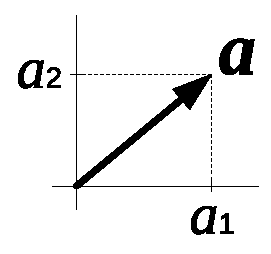
\includegraphics[keepaspectratio, width=3.1cm,height=3cm,clip]{chap9_ookisa001.pdf}
                \caption{2次元ベクトルの大きさ}
                \label{fig:chap9_ookisa001}
            \end{center}
        \end{figure}

        \subsection{基本演算}
        複数のベクトルがあるとき,ベクトル同士の演算を定義しておこう.
        ベクトルに対して定義される演算は,加算と減算と乗算であり,
        除算は定義されない.乗算には,
        定数倍,内積(スカラー積),外積(ベクトル積)の3種類がある.
        しかし,ここで言うベクトルの乗算は,
        普通の数で行われる乗算とは異なる概念であることに注意されたい
            \footnote{
                違いは,この後の説明で,自ずとわかるはず.
            }.
        ベクトルの演算が定義できるのは,すべてのベクトルの次元が同じ場合に限る.
        以下のベクトル演算の定義にでてくるベクトルは,すべて $n$ 次元
        ベクトルであると仮定する.次元が異なるベクトル同士の演算は定義しない.

        数学的な演算公理を示すことはせず,直感的にわかりやすい表現で
        演算の定義を示すにとどめておこう.

        \subsubsection{加算}
        2つの $n$ 次元ベクトル $\ba$,$\bb$ があるとき,
        この2つのベクトルに対する演算 $\ba+\bb$ を \textbf{加算} といい,
        次のように定義する.
        \begin{align}
            \ba + \bb   &:= (a_{1},\, a_{2},\,\cdots,\,a_{n}) + (b_{1},\,b_{2},\,\cdots,\, b_{n}) \notag \\
                        &=  (a_{1}+b_{1},\, a_{2}+b_{2},\,\cdots,\, a_{n}+b_{n} ).
        \end{align}

        成分を示す場合には,次のようになる.
        \begin{align}
            {(\ba+\bb)}_{i} := a_{i}+b_{i} \quad,\quad (i=1,\,2,\,\cdots,\,n).
        \end{align}
        添字の $i$ はベクトルの成分番号を示している記号である.式はすべての成分で
        成り立つが,すべての成分を書くと,上の定義のように,$i=1,\,2,\,\cdots,\,n$ の $n$ 通り
        を記述する必要が出てくる.しかし,どの成分番号に対しても,同じ形の式で
        定義で定義されることから,1から$n$の任意の一つを代表的に表す $i$ を導入した.

        \subsubsection{定数倍}
        スカラー $k$ と $n$ 次元ベクトル $\ba$ の積 $k\ba$ を \textbf{定数倍} といい,
        次で定義する.ここでは,$k$ を実数とする.
        \begin{align}
            k\ba := (k{a}_{1},\, k{a}_{2},\, \cdots,\, k{a}_{n}).
        \end{align}
        $\ba$ のすべての成分を $k$ 倍するということである.

        成分を示す場合には,次のように書く.
        \begin{align}
            {(k\ba)}_{i} := k{a}_{i} \quad,\quad  (i=1,\,2,\,\cdots,\,n).
        \end{align}

        \subsubsection{減算}
        加算と定数倍を定義しておけば,減算を定義する必要はない
            \footnote{
                一方に$-1$を乗じて(乗算)から,たし合わせればいい(加算).
            }.
        しかし,特徴的な演算であるため,この演算に \textbf{減算} という呼称を与える.
        減算は以下のような演算でのことをいう.2つの $n$ 次元ベクトル $\ba$,$\bb$ があるとき,
        ベクトルの減算 $\ba-\bb$ とは,
        \begin{align*}
            \ba-\bb &:= \ba + (-1)\bb \\
                    &= (a_{1}+(-1)b_{1},\, a_{2}+(-1)b_{2},\,\cdots,\, a_{n}+(-1)b_{n} ) \\
                    &= (a_{1}-b_{1},\, a_{2}-b_{2},\,\cdots,\, a_{n}-b_{n} )
        \end{align*}
        のような演算のことである.

        成分を示す場合には,次のようになる.
        \begin{align}
            {(\ba-\bb)}_{i} := a_{i}-b_{i} \quad,\quad (i=1,\,2,\,\cdots,\,n).
        \end{align}

        \subsubsection{内積(スカラー積)}
        2つの$n$次元ベクトル $\ba$,$\bb$ の内積 $\ba\cdot\bb$ とは,以下の演算のことをいう.
        \begin{align}\label{eq:chap9_naiseki001}
            \ba\cdot\bb := \sum_{i=1}^{n} a_{i}b_{i}.
        \end{align}

        展開したほうが,見やすいかもしれない(同じことを書いているだけ).
        \begin{align}
            \ba\cdot\bb := a_{1}b_{1} + a_{2}b_{2} + \cdots + a_{n}b_{n}.
        \end{align}

        演算結果がスカラーになることから,\textbf{スカラー積} ということもある.

        2次元ベクトルの場合,内積には図形的なイメージがある.
        それを強調した場合の,内積の定義は以下の通り.
        \begin{align}
            \ba\cdot\bb := |\ba||\bb| \cos \theta.
        \end{align}
        この定義は上の式(\ref{eq:chap9_naiseki001})の $n=2$ の場合と同値である.
        証明は後回し.
        \begin{figure}[htbp]
            \begin{center}
                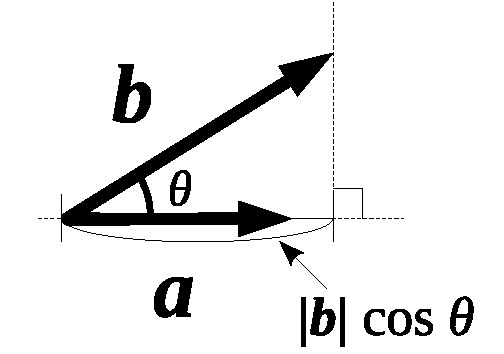
\includegraphics[keepaspectratio, width=4.23cm,height=3cm,clip]{chap9_naiseki001.pdf}
                \caption{内積}
                \label{fig:chap9_naiseki001}
            \end{center}
        \end{figure}

        \subsubsection{外積(ベクトル積)}
            \begin{mysmallsec}{外積の定義}
                2つの3次元ベクトル $\ba$,$\bb$ からなるベクトルの \textbf{外積} を
                $\ba\times\bb$ と表し,以下でその演算を定義する.
                    \begin{align*}
                            \ba \times \bb &:=& (\,
                                    a_{2}b_{3} - a_{3}b_{2},\;
                                    a_{3}b_{1} - a_{1}b_{3},\;
                                    a_{1}b_{2} - a_{2}b_{1}
                                \,)
                    \end{align*}

                演算結果がベクトルであることから,\textbf{ベクトル積} ということもある.

                唐突な定義で,無味乾燥だと思われるかもしれないが,
                根拠のあるものである.それを以下で説明しよう.
            \end{mysmallsec}

            \begin{mysmallsec}{一言}
                ベクトルの外積はわかりにくい.実際,定義式が少々複雑であり,図形的な
                イメージをすぐに描くには難しいかもしれない.しかし,ここを少々辛抱して
                手計算による練習をいくらかすることで,ベクトルの外積の意味やイメージを
                つかめるようになるはずである.
                ここでは,ベクトルの外積の定義を示すと共に,イメージを少しでも早くつかむ
                ことができるよう,丁寧に説明していく
            \end{mysmallsec}

            \begin{mysmallsec}{3次元ベクトルの外積のみを扱う}
                ここでの興味は3次元ベクトルの外積である.他の次元の外積は考えない.
                "興味がない"というのが直接的な理由だけれど,
                外積は内積のように簡単に $n$ 次元に拡張することができないことも,
                知っておいて損はないかも(多次元に拡張しようとして無駄な時間を費やさないように).

                外積の拡張に興味があれば,\textbf{外積代数} を学んでみる良い.
                外積代数は,ここでいう外積の自然な拡張ではないが(定義から違う),
                外積計算を発展させた形式の数学であることは実感できるだろう.
            \end{mysmallsec}

            \begin{mysmallsec}{定義の意味すること}
                ベクトルの外積とは,与えられた2つのベクトルから,
                この2つのベクトルの方向から独立した
                新しい方向を持つベクトルを1つ生成する演算である.
                その新しいベクトルの方向とは,2つのベクトルの両方に直交する方向であり,
                その大きさは $|\ba||\bb|\sin \theta$ である.
            \end{mysmallsec}

            \begin{mysmallsec}{外積の定義を知識0から作ろう}
                外積の定義の意味を実感するには,回り道かもしれないが,
                外積の定義に至るまでの思考プロセスをたどるとよい.
                先に示した外積の定義を一度忘れて,外積を1から作っていこう.
            \end{mysmallsec}

            \begin{mysmallsec}{外積の定義の目的}
                なぜ外積を定義したいのか.その理由は,外積を定義することにより,
                ある物理現象の数学的扱いが可能になるからである.必要は発明の母.
                力の釣り合いの解析には外積が欠かせないし,電磁気学ではローレンツ力
                を表すのに使われる.外積は闇雲に定義された演算ではなく,自然現象を
                詳細に観測した結果,それを説明するのに必要な演算方法なのである.
                自然現象の一部にはある特別な規則があり,それを数式で表そうとして
                試行錯誤して組み立てられた数学的概念が,外積なのである.
            \end{mysmallsec}

            \begin{mysmallsec}{外積演算に要求されること}
                2つの3次元ベクトル $\ba$,$\bb$ から,外積
                    \footnote{
                        今は,演算の名前なんてどうでも良い.知りたいのは
                        その具体的な演算方法である.この演算名は便宜的に
                        使用するものであり,"新しい演算方法"という
                        意味程度で捉えてもらいたい.
                    }
                によって生成したいベクトルの条件は以下の通りだった.
                \begin{enumerate}
                    \item 方向は $\ba$ と $\bb$ の両方に直交する方向である
                    \item 大きさは,$|\ba||\bb| \sin \theta$
                \end{enumerate}

                つまり,これから考えることは,
                \begin{enumerate}
                    \item 方向は 2つのベクトルに直交するようなベクトルをどう作るか.
                    \item さらに大きさを,$|\ba||\bb| \sin \theta$ にするには,どういう制約必要か
                \end{enumerate}
                の2点である.
                    \begin{figure}[hbt]
                        \begin{center}
                            \includegraphicslarge{gaiseki_01.pdf}
                            \caption{外積のイメージ}
                            \label{fig:gaiseki_01}
                        \end{center}
                    \end{figure}
            \end{mysmallsec}

            \begin{mysmallsec}{要求されることから,条件式を導く}
                2つの3次元ベクトル $\ba$,$\bb$ から,外積
                そのようなベクトルが仮に存在できたとして,それを $\bc$ と
                表すことにしよう($\bc:=\ba\times\bb$).

                $\bc$ は $\ba$ と $\bb$ の両方に直交しているから,内積が0になっているはずである
                    \footnote{
                        $\ba$,$\bb$ はともにゼロベクトルでないので(最初に要請される条件),
                        $|\ba| \neq 0$ ,$|\bb| \neq 0$ だから,$\cos(\pi/2)=0$ が
                        成立していなければならない.
                        $\ba$,$\bb$ の少なくとも一方がゼロベクトルである場合も外積は定義されるが,
                        この場合,新たに生成されるベクトルもゼロベクトルとなる特別な場合である.
                    }.

                したなら,次式が成立してなければならない.すなわち,
                    \begin{align*}
                        \ba \cdot \bc &= |\ba||\bc| \cos \frac{\pi}{2} = 0 \\
                        \bb \cdot \bc &= |\bb||\bc| \cos \frac{\pi}{2} = 0
                    \end{align*}
                である.
                ベクトル $\bc$ の成分を $(\,c_{1}\,,c_{2}\,,c_{3}\,)$ としよう.
                $\ba$ と $\bb$ についても同様に,
                それぞれ,$(\,a_{1}\,,a_{2}\,,a_{3}\,)$,
                $(\,b_{1}\,,b_{2}\,,b_{3}\,)$ とする.
                そうすると,上の2つの式は,また,以下のよう書いても同じことである.
                すなわち,
                    \begin{align*}
                        a_{1}c_{1} + a_{2}c_{2} + a_{3}c_{3} &= 0. \\
                        b_{1}c_{1} + b_{2}c_{2} + b_{3}c_{3} &= 0.
                    \end{align*}

                ベクトルの方向については,上の2式が成り立つことがその
                条件であるが,向きについては何も言っていない.
                そこで,次のように向きを決めてしまおう.すなわち,
                    \begin{description}
                        \item[向きの定義]
                            ベクトル $\ba$ とベクトル $\bb$ から生成する
                            外積 $\bc$ のむきは,
                            $\ba$ から $\bb$ に 向かって右ねじを右まわし回したときに,ネジが進む向きを,正方向とする.
                            これを満たすことを,\textbf{右手系をなす} という
                            別名「右ねじの法則」という表現が使われることも多い.
                    \end{description}

                    \begin{figure}[hbt]
                        \begin{center}
                            \includegraphicsdefault{migineji_01.pdf}
                            \caption{右ねじを回して進む方向}
                            \label{fig:migineji_01}
                        \end{center}
                    \end{figure}

                ベクトルにはもうひとつの性質である大きさ
                も考えないといけない.どのような大きさにしようと自由だが,
                最も簡潔に大きさを定めたい.もとの2つのベクトル $\ba$,$\bb$ より,
                この二つのベクトルが張る平行四辺形の面積を,その大きさと
                するのが最も簡単だろう.実際,数学的にもこのような定義が
                なされる.これが最も無理のない定義なのだろう.すると,
                $\bc$ の条件として,次式も加わることになる.
                    \begin{align*}
                        |\bc| &= | \ba || \bb | \sin\theta \\
                        &\Leftrightarrow \quad
                        \sqrt{{c_{1}}^{2}+{c_{2}}^{2}+{c_{3}}^{2}}
                        =
                        \sqrt{{a_{1}}^{2}+{a_{2}}^{2}+{a_{3}}^{2}}
                        \sqrt{{b_{1}}^{2}+{b_{2}}^{2}+{b_{3}}^{2}}
                        \sin\theta
                    \end{align*}

                これで,都合3つの条件式と,向きの定義は揃った.もう一度,まとめて書いておこう.
                \\
                \begin{itembox}[a]{外積演算で満たすべき条件式}
                    外積演算では,以下の条件式を満たさねばならない.
                    \begin{description}
                        \item[(1)] $a_{1}c_{1} + a_{2}c_{2} + a_{3}c_{3} = 0$ ($\bc \perp \ba$)
                        \item[(2)] $b_{1}c_{1} + b_{2}c_{2} + b_{3}c_{3} = 0$ ($\bc \perp \bb$)
                        \item[(3)] $\sqrt{{c_{1}}^{2}+{c_{2}}^{2}+{c_{3}}^{2}}
                               = \sqrt{{a_{1}}^{2}+{a_{2}}^{2}+{a_{3}}^{2}}
                                 \sqrt{{b_{1}}^{2}+{b_{2}}^{2}+{b_{3}}^{2}}
                                 \sin\theta$ (大きさ)
                        \item[(4)] $\ba,\,\bb,\,\bc$ は右手系をなす.(向き)
                    \end{description}
                \end{itembox}
                \\

                未知数が $c_{1}$,$c_{2}$,$c_{3}$ と三つなのに対し,
                条件式も同じく3つであり,数式的な条件としては必要十分である
                    \footnote{
                        これで,大きさと方向を定めることができる.
                    }.
                また,ベクトルの向きの定義もした.これで,外積を作る準備が
                整った.あとは,外積を作れるかどうか,言い換えれば,このように
                定義した外積というものが存在可能かどうかを,確認すれば良い.
            \end{mysmallsec}

            \begin{mysmallsec}{外積の成分表示}
                このような3式
                    \footnote{
                        正確には,「3つの式と,向きの定義」と書くべきだけど,
                        向きは人間が勝手に選ぶものなので,数式的に気にするもの
                        ではない.
                    }
                を満たすような $\bc$ は存在するのか.存在するとしたら,
                その成分はどのようになるか.それをこれから考えていこうと思う.それで,
                どうやって求めるかなんだけど,その方法は幾つか思い当たる.
                式をくどくどと計算をして発見的に答えを得る方法もあるけれど,
                それだと少々話が長くなり,計算も面倒くさい.なので,この問題の
                答えはすでに得られていることだから,先に答えを見てしまおう.
                そのほうが早い.

                で,その答えとは,
                    \begin{align*}
                        \bc &= (\,c_{1},\,c_{2},\,c_{3}\,) \\
                            &= (\,
                                    a_{2}b_{3} - a_{3}b_{2},\;
                                    a_{3}b_{1} - a_{1}b_{3},\;
                                    a_{1}b_{2} - a_{2}b_{1}
                                \,)
                    \end{align*}
                である.なにやら複雑な式に見えるが,次のように書くと,
                ある規則がみえてくるだろう.
                    \begin{align}\label{eq:VecGaiseki_Seibun}
                        \bc =
                        \left[
                            \begin{array}{c}
                                c_{1} \\
                                c_{2} \\
                                c_{3} \\
                            \end{array}
                        \right]
                        =
                        \left[
                            \begin{array}{c}
                                a_{2}b_{3} - a_{3}b_{2} \\
                                a_{3}b_{1} - a_{1}b_{3} \\
                                a_{1}b_{2} - a_{2}b_{1} \\
                            \end{array}
                        \right].
                    \end{align}

                $\ba$,$\bb$ の成分の添字を縦方向に意識して眺めると,
                巡回($1 \to 2 \to 3 \to 1$)しているのが見える
                    \footnote{
                        複雑そうに見えるけど,規則さえ分かってしまえば,
                        覚えるのはたやすい.最初の $a_{2}b_{3}$ さえ覚えてしまえば,
                        残りは機械的に記述できる.引く数は添字の数字を入れ替えた
                        ものだし,その他の成分については添字を巡回させればいい.
                    }.
                式(\ref{eq:VecGaiseki_Seibun})は,
                先ほど上げた3つの条件式を必要十分に満たす.
            \end{mysmallsec}

            \begin{mysmallsec}{外積の成分表示の検算}
                式(\ref{eq:VecGaiseki_Seibun})が本当に条件を満たすかどうかを,
                確かめておこう.まず,$\bc \perp \ba$,$\bc \perp \bb$ を
                満たすことを示す.やり方は,単純に条件式に成分を代入して,
                式を整理するだけである.

                条件式(1)について,
                    \begin{align*}
                         &a_{1}c_{1} + a_{2}c_{2} + a_{3}c_{3} \\
                         &\qquad=   a_{1}(a_{2}b_{3} - a_{3}b_{2})
                             + a_{2}(a_{3}b_{1} - a_{1}b_{3}) + a_{3}(a_{1}b_{2} - a_{2}b_{1}) \\
                         &\qquad=   a_{1}a_{2}b_{3} - a_{1}a_{3}b_{2}
                             + a_{2}a_{3}b_{1} - a_{2}a_{1}b_{3} + a_{3}a_{1}b_{2} - a_{3}a_{2}b_{1} \\
                         &\qquad= 0.
                    \end{align*}

                条件式(2)も同じように計算できる.
                    \begin{align*}
                         &b_{1}c_{1} + b_{2}c_{2} + b_{3}c_{3} \\
                         &\qquad=   b_{1}(a_{2}b_{3} - a_{3}b_{2})
                             + b_{2}(a_{3}b_{1} - a_{1}b_{3}) + b_{3}(a_{1}b_{2} - a_{2}b_{1}) \\
                         &\qquad=   b_{1}a_{2}b_{3} - b_{1}a_{3}b_{2}
                             + b_{2}a_{3}b_{1} - b_{2}a_{1}b_{3} + b_{3}a_{1}b_{2} - b_{3}a_{2}b_{1} \\
                         &\qquad= 0.
                    \end{align*}

                たしかに,二つの条件式を満たしている.このことにより,
                ベクトル $\bc$ は,ベクトル $\ba$,$\bb$ に直交している
                ことが確かめられた.つまり,ベクトル $\bc$ の方向は
                条件に沿うものであると言える.

                では,残りの大きさに関する条件式について,それを満たすか
                を計算してみよう.もう一度,大きさを決める条件式(3)を
                書くと,
                    \begin{align*}
                        &\sqrt{{c_{1}}^{2}+{c_{2}}^{2}+{c_{3}}^{2}}
                        =
                        \sqrt{{a_{1}}^{2}+{a_{2}}^{2}+{a_{3}}^{2}}
                        \sqrt{{b_{1}}^{2}+{b_{2}}^{2}+{b_{3}}^{2}}
                        \sin\theta
                    \end{align*}
                でるが,両辺を2乗して,
                    \begin{align*}
                        {c_{1}}^{2}+{c_{2}}^{2}+{c_{3}}^{2}
                        =
                        \left({a_{1}}^{2}+{a_{2}}^{2}+{a_{3}}^{2}\right)
                        \left({b_{1}}^{2}+{b_{2}}^{2}+{b_{3}}^{2}\right)
                        {\sin}^{2}\theta.
                    \end{align*}
                ここで,三角関数の公式 ${\sin}^{2}\theta + {\cos}^{2}\theta = 1$ を
                思い起こし,${\sin}^{2}\theta = 1 - {\cos}^{2}\theta $ と置き換えて,
                    \begin{align*}
                        &{c_{1}}^{2}+{c_{2}}^{2}+{c_{3}}^{2} \\
                        &\quad =    \left({a_{1}}^{2}+{a_{2}}^{2}+{a_{3}}^{2}\right)
                                    \left({b_{1}}^{2}+{b_{2}}^{2}+{b_{3}}^{2}\right)
                                    \left(1 - {\cos}^{2}\theta \right) \\
                        &\quad =    \left({a_{1}}^{2}+{a_{2}}^{2}+{a_{3}}^{2}\right)
                                    \left({b_{1}}^{2}+{b_{2}}^{2}+{b_{3}}^{2}\right) \\
                                    &\quad \qquad -\left({a_{1}}^{2}+{a_{2}}^{2}+{a_{3}}^{2}\right)
                                        \left({b_{1}}^{2}+{b_{2}}^{2}+{b_{3}}^{2}\right)
                                        {\cos}^{2}\theta.
                    \end{align*}
                最後の行の
                    \begin{equation*}
                        \left({a_{1}}^{2}+{a_{2}}^{2}+{a_{3}}^{2}\right)
                        \left({b_{1}}^{2}+{b_{2}}^{2}+{b_{3}}^{2}\right)
                        {\cos}^{2}\theta.
                    \end{equation*}
                に注目すると,
                    \begin{align*}
                        &\left(
                            \sqrt{{a_{1}}^{2}+{a_{2}}^{2}+{a_{3}}^{2}}
                            \sqrt{{b_{1}}^{2}+{b_{2}}^{2}+{b_{3}}^{2}}
                            {\cos}\theta
                        \right)^{2} \\
                            &\qquad=
                            \left(
                                \ba \cdot \bb
                            \right)^{2} \\
                            &\qquad=
                            \left(
                                a_{1}b_{1}+a_{2}b_{2}+a_{3}b_{3}
                            \right)^{2}.
                    \end{align*}

                つまり,大きさの定義式は以下のように書き換えられる.
                    \begin{align*}
                        &{c_{1}}^{2}+{c_{2}}^{2}+{c_{3}}^{2} \\
                        &\qquad =   \left({a_{1}}^{2}+{a_{2}}^{2}+{a_{3}}^{2}\right)
                                    \left({b_{1}}^{2}+{b_{2}}^{2}+{b_{3}}^{2}\right)
                                    \left(1 - {\cos}^{2}\theta \right) \\
                        &\qquad =   \left({a_{1}}^{2}+{a_{2}}^{2}+{a_{3}}^{2}\right)
                                    \left({b_{1}}^{2}+{b_{2}}^{2}+{b_{3}}^{2}\right)
                                    -   \left(
                                            a_{1}b_{1}+a_{2}b_{2}+a_{3}b_{3}
                                        \right)^{2}.
                    \end{align*}

                この式を,ベクトル $\bc$ が満たしていることを確認すればよい.
                    \begin{align*}
                        |\bc|^{2}
                        &=
                        {c_{1}}^{2}+{c_{2}}^{2}+{c_{3}}^{2} \\
                        &=
                         {(a_{2}b_{3} - a_{3}b_{2})}^{2}
                         + {(a_{3}b_{1} - a_{1}b_{3})}^{2}
                         + {(a_{1}b_{2} - a_{2}b_{1})}^{2} \\
                        &=
                        \left(
                            {a_{2}}^{2}{b_{3}}^{2} + {a_{3}}^{2}{b_{2}}^{2} - 2a_{2}a_{3}b_{2}b_{3}
                        \right)
                        + \left(
                            {a_{3}}^{2}{b_{1}}^{2} + {a_{1}}^{2}{b_{3}}^{2} - 2a_{1}a_{3}b_{1}b_{3}
                        \right) \\ &\qquad
                        + \left(
                            {a_{1}}^{2}{b_{2}}^{2} + {a_{2}}^{2}{b_{1}}^{2} - 2a_{1}a_{2}b_{1}b_{2}
                        \right) \\
                        &=
                          {a_{2}}^{2}{b_{3}}^{2} + {a_{3}}^{2}{b_{2}}^{2} + {a_{3}}^{2}{b_{1}}^{2}
                        + {a_{1}}^{2}{b_{3}}^{2} + {a_{1}}^{2}{b_{2}}^{2} + {a_{2}}^{2}{b_{1}}^{2} \\
                        &\quad - 2a_{2}a_{3}b_{2}b_{3} - 2a_{1}a_{3}b_{1}b_{3} - 2a_{1}a_{2}b_{1}b_{2} \\
                        &=
                          \left({a_{1}}^{2}{b_{3}}^{2} + {a_{1}}^{2}{b_{2}}^{2}\right)
                        + \left({a_{2}}^{2}{b_{3}}^{2} + {a_{2}}^{2}{b_{1}}^{2}\right)
                        + \left({a_{3}}^{2}{b_{2}}^{2} + {a_{3}}^{2}{b_{1}}^{2}\right) \\
                        &\quad - 2a_{2}a_{3}b_{2}b_{3} - 2a_{1}a_{3}b_{1}b_{3} - 2a_{1}a_{2}b_{1}b_{2}.
                    \end{align*}

                ちょっと一息.まだまだ式変形は続く.ちなみに,上式の冗長な括弧は,
                以降の式変形のために,明示的に記述している.

                次に,トリッキーな作業をする.それは,ある数 $x$ に対して,
                当然,$0=x-x$ が成り立つから,0を加えるということは $x-x$ を加えることと同じである.
                そして0を加えても等式は成り立つ.
                この考え方を利用して,式変形を続けよう.
                    \begin{align*}
                        |\bc|^{2}
                        &= {a_{1}}^{2}{b_{3}}^{2} + {a_{1}}^{2}{b_{2}}^{2}
                            + \left({a_{1}}^{2}{b_{1}}^{2} - {a_{1}}^{2}{b_{1}}^{2}\right) \\
                        &\quad + {a_{2}}^{2}{b_{3}}^{2} + {a_{2}}^{2}{b_{1}}^{2}
                            + \left({a_{2}}^{2}{b_{2}}^{2} - {a_{2}}^{2}{b_{2}}^{2}\right) \\
                        &\quad + {a_{3}}^{2}{b_{2}}^{2} + {a_{3}}^{2}{b_{1}}^{2}
                            + \left({a_{3}}^{2}{b_{3}}^{2} - {a_{3}}^{2}{b_{3}}^{2}\right) \\
                        &\quad - 2a_{2}a_{3}b_{2}b_{3} - 2a_{1}a_{3}b_{1}b_{3} - 2a_{1}a_{2}b_{1}b_{2} \\
                        &=   {a_{1}}^{2}\left({b_{1}}^{2} + {b_{2}}^{2} + {b_{3}}^{2}\right)
                           + {a_{2}}^{2}\left({b_{1}}^{2} + {b_{2}}^{2} + {b_{3}}^{2}\right)
                           + {a_{3}}^{2}\left({b_{1}}^{2} + {b_{2}}^{2} + {b_{3}}^{2}\right) \\
                        &\quad -{a_{1}}^{2}{b_{1}}^{2} - {a_{2}}^{2}{b_{2}}^{2} - {a_{3}}^{2}{b_{3}}^{2}
                               - 2a_{2}a_{3}b_{2}b_{3} - 2a_{1}a_{3}b_{1}b_{3} - 2a_{1}a_{2}b_{1}b_{2} \\
                        &=  \left( {a_{1}}^{2} + {a_{2}}^{2} + {a_{3}}^{2} \right)
                            \left( {b_{1}}^{2} + {b_{2}}^{2} + {b_{3}}^{2} \right)
                           -\left(a_{1}b_{1}+a_{2}b_{2}+a_{3}b_{3}\right)^{2}.
                    \end{align*}

                式変形が長々と続いたが,これでやっと確かめられた
                \footnote{
                    以下の恒等式が成立している.
                        \begin{equation*}
                            \left( X + Y + Z \right)^{2}
                            = {x}^{2} + {y}^{2} + {z}^{2} + 2XY + 2YZ + 2ZX.
                        \end{equation*}
                    ここでは,$X=a_{1}b_{1}$,$Y=a_{2}b_{2}$,$Z=a_{3}b_{3}$ に対応している.
                }.

                条件式(4)は,条件式(1)(2)(3)では特定することのできなかった向きを
                人為的に定めるものである.うるさいことを言うと,条件式(4)が条件式(1)(2)(3)に
                矛盾しないことを示すべきだが,割愛する.どちらの向きを正とするか,という問題
                であり,大げさに議論するところではない.単なる取り決めである.

                以上から,$\bc$ は3つの条件式を満たすことが確かめられ,ベクトルの外積が
                存在することが示された.つまり,ベクトルの外積は定義可能であることが確かめられた.
            \end{mysmallsec}

            \begin{mysmallsec}{最後に一言}
                何度も言うが,ベクトルの外積は導かれるものではない.人の想像力によって
                定義するものである.この外積という概念を導入することで,物体の回転を数学的に
                扱うことができるのである.というか,実際は話が逆で,ベクトルの外積の定義に従う
                物理現象が発見され,この現象を数学的に扱うことができるように,外積が定義される
                のである.もしかしたら,外積の定義が突拍子も無いと感じているかも知れないが,
                現実に外積を用いて説明される物理現象が生じているのである.外積はその現象を
                扱うために導入されるのだ.
            \end{mysmallsec}

                \begin{memo}{右手系とは何か}
                    外積の定義のうちの,向きの定義をもう一回読んでみよう.

                    \begin{description}
                        \item[向きの定義]
                            ベクトル $\ba$ とベクトル $\bb$ から生成する
                            外積 $\bc$ のむきは,
                            $\ba$ から $\bb$ に 向かって右ねじを右まわし回したときに,ネジが進む向きを,
                            正方向とする.これを満たすことを,\textbf{右手系をなす} という.
                    \end{description}


                    なぜこのように定義するのかという疑問があろうが,この疑問
                    はすぐに捨て去るべきだ.なにしろ,答えがないのだから.
                    しかし,天下り的な説明はよくない.なので,できるだけ
                    “もっともらしい”説明を,以下に記述しておくことにしよう
                        \footnote{
                            あくまでも,“もっともらしく”記述するのであり,
                            これがほんとうの理由だとか,正解だとかというものではない.
                            天下り的な説明ではスッキリとせず,モヤモヤしてしまう
                            ので,これを少しでも解消できればと考えて,記述
                            するものである.
                        }.

                    2つのベクトル $\ba$,$\bb$ に直交する方向は内積の数式で表現され,
                    数学的に議論できるが,方向は計算で導くことはできない.なので,
                    予め,向きを定めておくのである.どちらの向きを正方向としても,
                    それ以降で変更しなければ,論理に矛盾は生じない.しかし,向きを
                    決めないと議論ができないので,人為的な向きの定義を施すのである.

                    では,なぜ,「右ネジをまわして進む向き」と表現するのか.
                    これにも,多分,明確な答えはない.
                    おそらく,これが最も簡潔な言い回しで,誤解なく,加えて直感的イメージ
                    しやすく説明できるからだろう.しかし,学術的には格好をつけて,
                    「右手系をなす」と言われる.それは,右手の親指を人差し指に近づけるという
                    行為が,親指を右まわしするという行為に当たり,中指の先の向きが
                    外積の向きに一致するからである.元となる2つのベクトルが親指と人差し指に
                    値し,それに直交する向きに中指が向いているのだ.
                    \begin{figure}[hbt]
                        \begin{tabular}{cc}
                            \begin{minipage}{0.5\hsize}
                                \begin{center}
                                    
\includegraphics[keepaspectratio, width=3cm,height=3.75cm,clip]{migitekei_TE_2.pdf}

                                    (a) 右手
                                    \label{fig:migitekei_TE_mono_x}
                                \end{center}
                            \end{minipage}
                            \begin{minipage}{0.5\hsize}
                                \begin{center}
                                    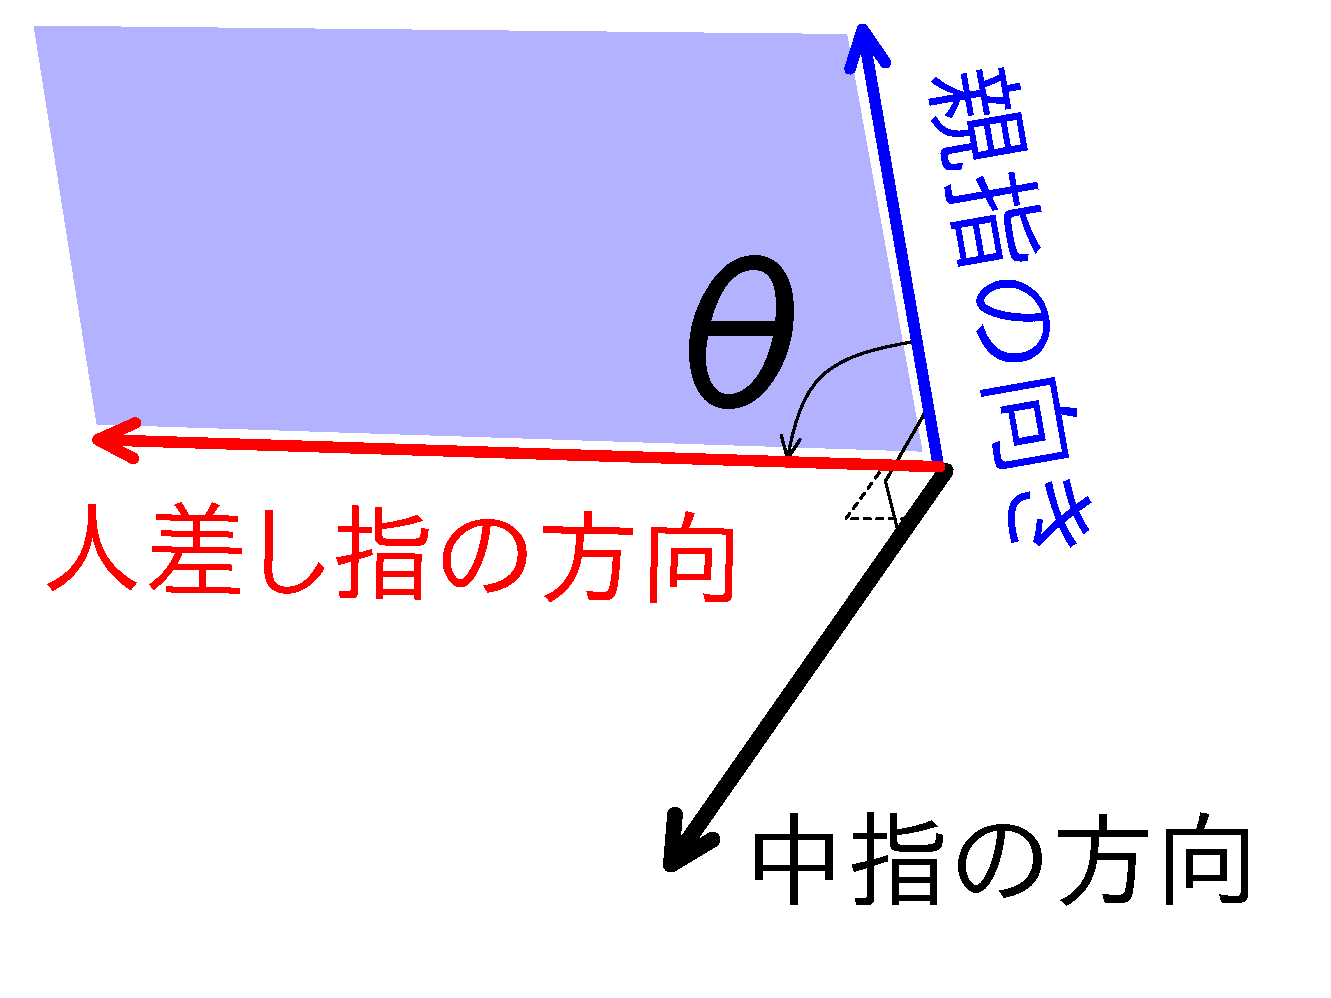
\includegraphics[keepaspectratio, width=3cm,height=3.75cm,clip]{migineji_Myhand.pdf}

                                    (b) 対応図
                                    \label{fig:migineji_Myhand}
                                \end{center}
                            \end{minipage}
                        \end{tabular}
                        \caption{右手系}
                    \end{figure}
                \end{memo}

        \subsubsection{乗算?}
            ベクトルの乗算を,加算と同じように定義できないだろうか.
            つまり,2つの $n$ 次元ベクトル $\ba=(a_{1},\,a_{2},\,\cdots,\,n)$,
            $\bb=(b_{1},\,b_{2},\,\cdots,\,n)$ を用いて,
                \begin{equation*}
                    {(\ba \ast \bb)}_{i} = a_{i}b_{i}
                \end{equation*}
            と定義してはだめか
                \footnote{
                    記号に $\ast$ を使った理由は,内積の記号に $\cdot$,
                    外積の記号に $\times$ が使われるため,これらと区別
                    したかったためである.
                }.
            先人がこのように定義をしていないからには,
            できない理由があるに違いない.しかし,このように
            乗算を定義しても,不整合が起きるわけでもなく,定義不可能
            とは思えず,むしろ定義可能であると思えて仕方ない.
            私の力では,この定義を採用しない強い理由を見つけられない.

            しかし,このような乗算を定義してしまうと,ベクトルと数の違いが全く
            なくなってしまうことは確かだ
                \footnote{
                    実際に試してみてほしい.数と全く同じで,ベクトルを
                    定義した意味が全く感じられないことだろう.
                }.
            つまり,ベクトルとは表記上の利便性が向上
            しただけで,数学的な新しい概念となるわけではなくなる.
            数学的な発展を考えた場合,このような仕方の冗談の定義では
            前進がないので無駄ということになる.要するに,こんな乗算を定義
            してしまっては,わざわざベクトルを定義したことが無意味になって
            しまうのだ.表記方法を工夫しただけで新しい数学的概念とは言えない.
            もちろんこれでは,物理学にとっても,何のご利益もない
            ものになってしまうことだろう.
            だから,むしろ意識的に,このような定義を避けているのではない
            かと思われる(確証はない).ベクトルに内積や外積を定義することで,
            物理学に有用な数学になると共に,とても興味深い数学的対象となる.

        \subsubsection{除算??}
            ベクトルの内積の定義を採用すると,
            ベクトルの除算を定義することは難しい,と悟るのは容易だろう
            \footnote{
                $\bX\cdot\ba=k$ のとき,単純に $\ba=k/\bX$ とはできそうにない.
                $\bX$ をベクトルの変数とみなしたときに,この式を満たす $\bX$ は
                無限に存在するするから,できるとするならば,何か条件や約束事が必要だが,
                いい案は思い当たりそうにない.例えば,無限に存在する解をひとまとめにして,
                "解空間"(微分方程式など解空間とはべつもの)なるものをでっち上げたとしても,
                これ以上の発展は見込めないだろう.
            }.

            上記の "$\ast$" 乗算が採用されるのであれば,同じように除算を
            定義することは可能である.それは単に数を並べただけなので,
            吸うと全く同じ四則演算を定義すれば,不整合は起こらない.
            上記の乗算を定義しない理由に従うと,内積や外積を定義した方が
            学問的に有益である.そうなると,除算の定義が格段に難しくなる,
            というか,定義できたとしても条件が複雑すぎて,つまらなくなるだけだろう.

            だから,除算が定義できないのではなく,学問的に有益でないから定義しない
            と言ったほうが,正確なのであろう.

            数における0除算の禁止も,数学的に有益ではないから定義しないのだ,言えなくもない.
            よく挙げられる0除算が禁止される理由として,それを仮定すると不整合が起きるからだ
            といった説明がなされることがある
                \footnote{
                     $a$ を任意の数とするとき,$a \cdot 0 = 0$ が成立する(0の存在公理).
                     このとき,$a \neq b$ なる $b$ をもってきても $b \cdot 0 = 0$ である.
                     よって,$a \cdot 0 = b \cdot 0$(ここまでは正しい).
                     \textbf{両辺を0で割ると} $a=b$ となるが,これは $b$ の最初の条件に
                     矛盾する(不整合の発生).よって,0除算は禁止とされる.
                }.
            しかし,これは決して論理的な説明でない(美しい言い訳ではあるけれど).
            不整合が起きないように定義しなおせばよい.
            数学の論理は自然に存在するものではなく,人間が勝手気ままに構築
            するものであるから,定義なんていくらでも好き勝手できるはずである.ただ,
            0除算が定義できるようなうまい約束事を見つけられたとしても,複雑怪奇な理論
            が出来上がることになるのだろう(そんな理論に誰が興味を持つだろうか).

        \subsection{分解}
        1つのベクトルを複数のベクトルに分割することも可能である.
        例えば,$\ba = \bb + \bc$ が 成立しているとき,
        ベクトル $\ba$ は 2つのベクトル$\bb$と$\bc$に分割可能である.
        等式が成立していれば,分割するベクトルの個数に際限はない.
        このように,1つのベクトルを,加算が成り立つように複数のベクトルに
        分割することを,ベクトルの \textbf{分解} という.

        \subsection{単位ベクトル}
        大きさが1のベクトルを \textbf{単位ベクトル} という.
        単位ベクトルの記号は教科書により様々である.
        このノートでは,$\bn$ を単位ベクトルの記号として使用する
        \footnote{
            ただし,常にこの記号を用いるわけではない.その場合は,その直前か直後
            に説明を書くこととする.
        }.

        定義から,以下が成立する($n$ 次元を想定).
        \begin{align}
            |\bn| = \sqrt{\sum_{n=1}^{n} {n_{i}}^{2}} = 1.
        \end{align}
        $n_{i}$ のそれぞれの値には興味はないが,上記の関係式を満たす.
        単位ベクトルの方向は問わない.

                \subsection{演算の諸性質(公式)}
        \begin{mycomment}
            ベクトル基本的な演算性質を記しておく.
            $\ba$,$\bb$,$\bc$,$\bd$ はベクトルで,$k$,$l$ はスカラーである.
            括弧の内部の計算は,それがない部分よりも,優先度が高い(先に計算すべき)とし,
            それ以外の計算は左から順に計算する.
        \end{mycomment}

        \subsubsection{加算と定数倍に関する公式}
            ベクトルの加算と定数倍に関する演算性質は,スカラーの場合と変わらない.
            代表的な演算を以下に書いておく.
            \begin{enumerate}
                \item $\ba + \bb = \bb + \ba$
                \item $(\ba + \bb ) +\bc = \ba + (\bb + \bc)$
                \item $k (\ba + \bb) = k\ba + k\bb$
                \item $k(l\ba) = l(k\ba) =(kl)\ba$
                \item $\ba = \ba + \bzero = \bzero + \ba$
                \item $\ba +(-1)\ba = \bzero$
                \item $1\ba = \ba$
            \end{enumerate}

            以下,簡単に説明を与えておく.
            \begin{enumerate}
                \item 項の順序を入れ替えてから加算しても,結果は変わらない.\textbf{交換法則} とよばれる.
                \item 加算の順番を入れ替えても,結果は変わらない.\textbf{結合法則} とよばれる.
                \item 加算と定数倍に関する性質.
                      加算してから定数倍しても,両者を定数倍してから加算しても,どちらも
                      同じ結果になる.\textbf{分配法則} とよばれる.
                \item スカラーのかける順番を変えても,結果はわらなない.
                \item ゼロベクトル $\bzero$ を足しても結果は変わらない.
                      法則ではなく,$\bzero$ の存在を認めるもの.
                \item ベクトルから自身を引くとゼロベクトルになる.
                      $(-1)\ba$ は $\ba$ の \textbf{逆ベクトル} という.
                      $\ba$ も $(-1)\ba$ の逆ベクトルである(逆ベクトルの一意性).
                \item スカラーの1倍の1は記述を省略できる.
            \end{enumerate}

            どれも,定義から丁寧に計算すれば自明であるので,証明するまでもない
            \footnote{
                本音は$\cdots$
                \begin{itemize}
                    \item "記述が面倒だから省略させてほしい" という甘え
                    \item "書いたところで,ノートの記述が煩雑になって読みにくくなる" という言い訳
                    \item "自分で計算すれば,理解の確認になるのではないか" という逃げ
                \end{itemize}
                である.

                証明するには,式の両辺を独立に成分計算し,
                対応する成分同士が等しいことを確認すればいい.
                一意性を示したい場合には,異なる2つのものがあると仮定しても,
                両者が同値になることを示せばいい.
            }.

        \subsubsection{内積に関する公式}
            内積もスカラーと同じように扱える.主な性質は以下の通り.
            \begin{enumerate}
                \item $\ba \cdot \ba = {|\ba|}^{2}$
                \item $\ba \cdot \bb = \bb \cdot \ba$
                \item $\ba \cdot (\bb + \bc) = \ba \cdot \bb + \ba \cdot \bc$
                \item $(\ba + \bb) \cdot \bc = \ba \cdot \bc + \bb \cdot \bc$
                \item $k(\ba \cdot \bb) = (k\ba) \cdot \bb = \ba \cdot (k\bb)$
                \item $\ba \parallel \bb \Leftrightarrow \ba \cdot \bb = 0$
                \item $\ba \perp \bb \Leftrightarrow \ba \cdot \bb = \displaystyle\frac{\pi}{2}$
            \end{enumerate}

            言葉でも説明しておこう.
            \begin{enumerate}
                \item 自身の内積は,自身の大きさの2乗に等しい.
                \item 内積の項の順序を入れ替えても,結果は変わらない.
                \item 分配法則が成り立つ
                \item 分配法則の別の形(1と2より自明だろう)
                \item 定数倍と内積に関して,結合法則が成り立つ.
                \item 2つのベクトルが平行であることと,それらの内積が0であることは等価
                \item 2つのベクトルが垂直であることと,それらの内積が$\displaystyle\frac{\pi}{2}$であることは等価
            \end{enumerate}

            \begin{mysmallsec}{内積の使い所}
                物理学でベクトルの内積を使う場合は,2つのベクトルの交わりの角度を気にする場合が
                ほとんどである.平行なのか,垂直なのか,そうでなければどんな角度で交わっているのかが,
                内積の計算によってわかるからである.
            \end{mysmallsec}

        \subsubsection{外積に関する公式}
            外積の演算性質は,他とは異なるので,注意が必要である.
            \begin{enumerate}
                \item $\ba \times \ba = \bzero$
                \item $\ba \times \bb = - \bb \times \ba$
                \item $\ba \times (\bb \times \bc) = (\ba \cdot \bc) \bb - (\ba \cdot \bb) \bc $
            \end{enumerate}

            簡単にコメントを書いておく.
            \begin{enumerate}
                \item 自身の外積はゼロベクトルである.
                \item 外積の項の順序入れ替えると,符号が反転する.
                \item \textbf{ベクトルの三重積} という異名をもつ.
                      ちなみに,右辺の $\ba \cdot \bc$,$\ba \cdot \bb$ の演算結果はスカラーである.
            \end{enumerate}

            他にもたくさんあるけど,省略する.ベクトルの外積に関する公式は,
            一見して複雑な形をしたものが多く(検算が大変),挫折しがちだ.
            しばらく見ていると規則性が見えてきて,美しく感じるのかもしれないが,
            頻繁に使うのは上の3つくらいだ.後は,必要になったらときに,公式集を参照しよう.

        \subsubsection{単位ベクトルに関する公式}
        任意のベクトルは,同じ向きの単位ベクトルの定数倍である
            \footnote{
                証明はしないけど.
            }.
        アタリマエのことを言っているようだが,確認しておこう.
        ある $n$ 次元ベクトルを用意して,$\bX$ としよう.
        単位ベクトルの向きは,$\bX$ と同じとする.
        $\bX$ を単位ベクトル $\bn$ の定数 $k$ 倍と表せたとすると,$\bX = k\bn$ と
        なる.$\bX=(X_{1},\,X_{2},\,\cdots)$,$\bn=(n_{1},\,n_{2},\,\cdots,\,n)$ とすると,
            \begin{equation*}
                X_{i} = kn_{i} \quad,\quad (i=1,\,2,\,\cdots,\,n)
            \end{equation*}
        が成り立つ.これを踏まえて,$\bX$ の大きさ $|\bX|$を考えてみよう.
        簡単な計算で,$|\bX|=k$ が導ける.
            \begin{equation*}
                |\bX| = \sqrt{\sum_{n=1}^{n} {X_{i}}^{2}}
                      = \sqrt{\sum_{n=1}^{n} {(kn_{i})}^{2}}
                      = k \left(\sqrt{\sum_{n=1}^{n} {n_{i}}^{2}}\,\right)
                      = k \cdot 1
                      = k.
            \end{equation*}
        ここで,単位ベクトルの大きさが1であることを使用した.

        以上から,任意のベクトルは単位ベクトルを自身の大きさで定数倍したものに等しい,と言える.
        式で書くと,次の通り.
        \begin{align}
            \bX = |\bX|\bn.
        \end{align}

        上式を逆手に考えて,
        \begin{align}
            \bn = \frac{\bX}{|\bX|}= \frac{1}{|\bX|} \bX.
        \end{align}
        と見ることで,任意のベクトルの単位ベクトルを計算することもできる.

        しかし,次は無意味であることに注意しておくこと.
        \begin{align*}
            \mbox{(意味のない式)}\quad|\bX| = \frac{\bX}{\bn}
        \end{align*}
        ベクトル同士の除算は定義されておらず,この式は何も意味しない.


%%%        %======================================================================
%  Chapter : ベクトル解析
%  説明    : 電磁気学を記述する上で必要なベクトル解析のまとめ
%======================================================================

%======================================================================
%  Section
%======================================================================
    \section{ベクトル解析}
    \subsection{ベクトル変数(あるいは,変数ベクトル)}
    ベクトルには,スカラーにおける語彙「変数」に対応する,一般的呼称がない.
    ないと不便なので,このノートでは \textbf{ベクトル変数} という言い方を導入する.
    もしかしたら,\textbf{変数ベクトル} と書くこともあるかもしれない.

    細かいことを言うと,ベクトル変数は,
    成分の一部あるは全部が変数であるようなベクトルであり,
    次に説明するベクトル関数である
        \footnote{
            定義が論理的に循環してしまっているが,意図は伝わるはず.
            循環しないような記述も可能だが,理論構築が目的ではない
            ため,深く突っ込まないでおこう.
        }.

    変数をベクトル変数と区別する意味で,\textbf{スカラー変数} と
    書くこともある.

    \subsection{ベクトル関数}
    ベクトルが絡む関数のことを総称して \textbf{ベクトル関数} という.
    また,ベクトル関数と区別するために,
    今まで考えてきたベクトルが絡まないような関数を,
    \textbf{スカラー関数} と表現する場合がある
        \footnote{
            細かいことを言うと,スカラーは1次元ベクトルだから,
            スカラー関数もベクトル関数である.
        }.

    考えれる例をいくつか上げておこう.特にこれらを区別してよぶ必要は
    ないので,名称を与えることはしない
        \footnote{
            記述の際には,どんな形の
            ベクトル関数について議論している
            かが明確にわかるようにする.
        }.

    例えば,スカラーの独立変数 $t$ に対して,
    1つの定ベクトルが定まる関数が考えられる.これを
        \begin{align}
            \ba (t)
        \end{align}
    と表す.
    関数記号 $\ba$ を太字にした意図は,
    ベクトルが定まる(値域がベクトルである)ことを明示するためである.
    また,$(t)$ という表記は,$t$ が独立変数であることを示すものである
        \footnote{
            多変数になる場合,$\ba(t,\,s)$ と書かれることになる
            ($t$ と $s$ はスカラーである).
            このとき,$(t,\,s)$ という記述がベクトルを成分表示と同じで,
            紛らわしいかもしれない.しかし,文脈により容易に区別できる
            とし,特に書き分けることはしない.この記述の前に関数を
            表現する文字があれば,それらは独立変数である.
        }.

    別の例を上げると,ベクトル変数を独立変数にもつ関数が考えられる.
    数式で表そうとすると,
        \begin{align}
            \ba (\br)
        \end{align}
    のようになる.$\br$ はベクトル変数である.

    上記2つの混合して,スカラー変数 $t$ とベクトル変数 $\br$ から
        \begin{align}
            \ba (t,\,\br)
        \end{align}
    という関数を作ってもいい.

    ベクトル変数を独立変数として,スカラーが定まる(値域がスカラーである)
    関数もあり得る.記号化すれば,
        \begin{align}
            a (\br)
        \end{align}
    となるだろう.関数記号 $a$ を細字にした意図は,スカラーが定まることを
    明示するためである.

    もちろん,スカラー変数 $t$ とベクトル変数 $\br$ をもち,
    スカラーが定まる関数も考えられる.
        \begin{align}
            a (t,\,\br)
        \end{align}

    定ベクトルもベクトル関数の一部として考える.
    明示的な独立変数はないが,入力にかかわらず常に一定値をとるような
    関数として捉える.スカラー関数の場合と同じように考える.

    独立変数が1つのベクトル関数($\ba(t)$)を,\textbf{1変数ベクトル関数} という.
    独立変数が2つ以上のベクトル関数を総称して,\textbf{多変数ベクトル関数} という.
    ベクトル変数をもつベクトル関数($\ba(\br)$ など)は多変数ベクトル関数として考える.

    ひと目で見やすいように,表にしておこう(\Table\ref{table:f4unit}).
        \begin{table}[htb]
          \centering
          \caption{ベクトル関数の種類}
          \begin{tabular}{|l|c|c|l|}                                        \hline
            関数記号      & 独立変数   & 値域     & 例                      \\ \hline  \hline
            $\ba$         & なし       & ベクトル & 定ベクトル              \\ \hline
            $\ba(t)$      & $t$        & ベクトル & ある1点の風向の時間推移 \\ \hline
            $\ba(\br)$    & $\br$      & ベクトル & ある時刻の風向分布      \\ \hline
            $\ba(t, \br)$ & $t$,$\br$ & ベクトル & 風向分布の時間推移      \\ \hline
            $a(\br)$      & $\br$      & スカラー & 風力分布                \\ \hline
            $a(t, \br)$   & $t$,$\br$ & スカラー & 風力分布の時間推移      \\ \hline
          \end{tabular}
          \label{table:f4unit}
        \end{table}

    \subsection{ベクトル関数の微積分}
    \begin{mycomment}
        スカラー関数での微積分を,ベクトル関数へ拡張する.
        ベクトル関数の微積分も,基本的にはスカラー関数と同じように
        計算可能である.
    \end{mycomment}

    \subsubsection{極限}
    ベクトル関数の極限はスカラー関数の場合と同じように定義できる.

    \subsubsection{導関数}






%%%
%===================================================================================================
%  Chapter : 電磁気学が対象とする現象
%  説明    : 電磁気学の対象となる,電気的現象・磁気的現象の実在についての確認をする
%===================================================================================================
\chapter{電磁気学が対象とする現象}
%   %-----------------------------------------------------------------------------------------------
%   %  Input
%   %    File Name : PhysNote_EM_1st_Intro.tex
%   %    説明      : 電磁気学を構成する基本的な概念を説明する.
%   %-----------------------------------------------------------------------------------------------
        %===================================================================================================
%  Chapter : 電磁気学が対象とする物理現象
%  説明    : 電磁気学の対象となる,電気的現象・磁気的現象の実在についての確認をする
%===================================================================================================

%======================================================================
%  Section
%======================================================================
    \section{はじめに}\label{sec:EM_ObjPreMsg}
        \begin{mycomment}
            本節では,以降の電磁気学への導入と,これからの電磁気学の
            学習の段取りを説明する.
        \end{mycomment}

    %======================================================================
    %  SubSection
    %======================================================================
    \subsection{電気と磁気}\label{subsec:ElcAndMgn}
        これから学習する電磁気学は,\textbf{電気} と \textbf{磁気} が起こす
        様々な現象を説明する物理学の分野の1つである.
        電気とか磁気とかというと,日常的に用いられている使い慣れた言葉であり,
        そのイメージも多くの人々が共有している.「何を今更」と思われるかもしれないが,
        今まで日常的に使われてきた「電気」とか「磁気」とか
        という言葉と,そのイメージを一度整理しておきたい.
        これから学習する電磁気学は,電気とは何か,あるいは,磁気とは何かを
        探求するものであり,その疑問となる根本的な現象についてを確認せずに
        話を進めるには,甚だ滑稽なことだろう.

    %======================================================================
    %  SubSection
    %======================================================================
    \subsection{電気と磁気の伝わり方}%\label{subsec:ElcAndMgn}
        私達の感じてる電気や磁気は,実際には,静電気の引力
        (あるいは斥力)というように,力として現れている.つまり,力の伝達の
        表現方法が必要になってくる.
        “力の伝達”と聞いて,なんのことだ? と思ったかもしれない.
        というのも,ニュートン力学では,力の伝播については無視していたからである.
        そこでは,暗黙の了解として,「力は瞬間的に,つまり,時間0で伝わる」
        ということが仮定されていたのだ.しかし,このような考え方では,無限に遠くに存在する
        物体にも,近隣に存在する物体にも,力が "同時" に伝わる事になってしまう.
        これは直感に反するのではないだろうか.近くにある物体には,すぐに力が
        伝わり,遠くにあるものほど力の伝わり方が遅いというように,
        力の伝播に時間がかかるとしたほうが,自然な考え方では
        なかろうか.まあ,何れにしても,実験的に確かめないといけないところ
        だが,現在では,一般相対性理論で説明されるとおり,力の伝播には,時間
        がかかることがわかっている.つまり,力が一瞬で伝わると仮定されている
        ニュートン力学は,この部分において,間違っている.その間違いの修正は
        追々やっていくとして,ここでは,力の伝播をどうやって式で表現できるか
        を考えないといけない.
        そこで,力の伝播を表現するための概念である,\textbf{場} という考え方が
        導入される
            \footnote{
                小言を言っておこう.

                「場」という考え方は自然な考え方であるが,概念が抽象的すぎて,
                なかなか初学者にとって受け入れ難いことだろう.
                しかし,我慢して欲しい.「場」という考え方は,これからいっそう重要に
                なってくる.現代の物理学は,「場」という考え方が理論構築の基礎になっているからである.
                はじめに「場」ありき,という考えが一般的なのだ.
                理由はわからないが,そういう考え方のもとで,理論構築をし,成功を収めている.

                この部分は,"自然だけども特殊な考え方"なので,
                最初学習する上でつっかえる所だろう.理解するのに,
                時間がかかってしまうが,悩まずに,学習を進めていってもらいたい.
                数式とそのイメージをリンクさせようともがきながら
                (いろいろ考えたり,ヒントとなる本,Webサイトを探したりしよう)
                学習を進めれば,いつの間にか,「場」という考え方に慣れて
                (毒されて?)しまうものである.

                こんなことをここで言うな,と言われるかもしれない.実際そのとおりで,
                あとでまた同じ事を言うことだろう.ここでは,“この先に困難がありますよ”
                という案内として記述したまでである.
                (RPG風に言うなら,「(王様の台詞) 勇者よ,お前はこれから多くの困難に直面
                することだろう.しかし,それに屈してはならない.どんな困難だろうとも,
                それに立ち向かい,解決せねばならない.いかなる困難も克服し,壮大な目標に
                向かって,前進するのだ.行け,勇者よ,そして,いつの日か目的を果たし,
                帰還するのだ.」といった感じだ.)
            }.

    %======================================================================
    %  SubSection
    %======================================================================
    \subsection{電気・磁気の研究の歴史(ダイジェスト)}
        電磁気学で着目する力は,\textbf{電磁気力} と言われる.これは,
        \textbf{電気的な力} と \textbf{磁気的な力} の両方を指す言い方
        である.電気的な力や磁気的な力の存在自体は,摩擦時に起こる静電
        気や磁石の存在から,古くから知られていたことだろう.
        しかし,その力の持つ性質を科学的に扱うことができるのは,16世紀
        になってからである.ギルバート
            \footnote{
                William Gilbert(1544--1603, イギリス):Gilberd と
                表現されることもある.電磁気現象を近代的な実験方法で
                研究した,最初の人物のひとりとして有名である.検電器
                を発明している.医者としての仕事の傍ら,電磁気の研究
                をしていたらしい.
            }
        による電磁気現象の研究が,電磁気学の幕開けとするのが通説のようである.
        しかし,より正確に電磁気現象が扱えるようになるのは,
        キャベンディッシュ
            \footnote{
                Henry Cavendish(1731--1810, イギリス):化学と物理学
                の研究で有名.人間嫌いであったり,研究した結果を秘密
                にしておいたりと,特異な性格を強調されることが紹介さ
                れる言が多い(あ,ここにも書いてしまった).地球の
                比重を測定したことでも有名.これにより,万有引力の存
                在の裏付け,並びに,地球の重力定数の測定がなされた.
                また,電磁気学に関して言えば,クーロンの法則をクーロ
                ンよりも前に発見したことが,キャベンディッシュ死後に,
                マクスウェル(※1)より明らかにされている.

                (※1)James Clerk Maxwell(1831--1879, イギリス).
                \ref{subseq:4fundlaw_Hajimeni}節の脚注を参照.
            }
        やクーロンが電気的な力のもつ性質を実験的に解析する18世紀ごろである.
        アンペール
            \footnote{
                Andre-Marie Amp\'{e}re(1775--1836, フランス):電流に関
                する実験で有名.電流の単位「アンペア[A]」は彼の名にちなん
                だものである.
            }
        による電流と力の関係
            \footnote{
                この関係は,アンペールの法則と言われる.詳しいことは,後述する.
            }
        の発見や,ビオ
            \footnote{
                Jean-Baptiste Biot(1774--1862, フランス):物理学者であり,
                数学者,天文学者でもある.後に述べる,ビオ$=$サバールの法則
                の発見者のひとりとして有名.大気圧の測定も行っていたらしい.
            }
        とサバール
            \footnote{
                F\'{e}lix Savart(1791--1841, フランス):ビオと共同で,
                ビオ$=$サバールの法則を提唱したことで有名.カタカナ表記では,
                「サヴァール」と書いたほうが,正確なのかもしれない(だけど,
                このノートでは「サバール」と書くことにしたい.こっちのほうが
                見慣れたカタカナので,つっかえることなく読めると思う).
                外科医でもあったらしい.また,現在の音程の単位はセント(1
                オクターブ$=$1200セント)であるが,それ以前の単位として,
                サバール(savart)が使われていた.ちなみに,音程1サバールは
                だいたい4セントくらいである(なので,だいたい1オクターブは
                300サバールということになるのか).
            }
        の磁気と電流の関係の研究もだいたい19世紀初期に行われていている.最終的な
        電磁気学の確立がマクスウェルによってなされるのが19世紀中頃(1864年)である.

        電磁気現象は古くから知られていたのに対し,その現象を科学的に
        扱えるようになるのは,19世紀中頃になってからであった.そもそも科学という
        考え方自体が,ルネッサンス期に芽生えたものとされているので,仕方がないの
        かもしれないが,それにしても,電磁気現象を人間が把握するのに,これだけの時間が
        かかっているのには驚きである
            \footnote{
                話がそれるが,今日ある私たちの生活環境は,
                パソコンや携帯電話など,電磁気学を応用して作り
                出されている.そう,私たちの掌の中には,それだけの
                研究の重さがのしかかっているのである.ただ持っているだけでは
                なんにも感じないけど,少し学習すると,それらの機器を見たとき,
                先人の研究努力に対し,感謝の気持ちを懐くことだろう.
            }

%======================================================================
%  Section
%======================================================================
    \section{電気的現象}
        世の中には,接触していないにもかかわらず,力を受けることがある.
        この非接触で感じる力の中に,\textbf{電気的な力} がそのひとつとして
        存在する.

        例えば,髪の毛を下敷きでこすり,その後すぐに下敷きを頭の上の方へゆっ
        くりと持ち上げてみると,髪の毛は下敷きに吸いつけられるかのように持ち
        上がる.この現象を,一度は,小学生のころに実験や遊びで経験したことと思う.
        \textbf{電気的現象} の一例として,頻繁に頻繁にあげれる現象だ.
        この現象を物理学的には電磁気学で説明される.
        特に,静電気学として語られることが多い.
        静電気学は,電磁気学でも最も基本となる考え方である.
        になる.

%======================================================================
%  Section
%======================================================================
    \section{磁気的現象}
        非接触的に受ける力の別の例として,\textbf{磁気的な現象} も考えられる.
        鉄などの特定の金属をひきつける
            \footnote{
                ひきつける:相対的に考えれば,「引き寄せられる」といっても同
                じこと.
            }
        石がこの世界には存在し,日本では \textbf{磁石} と呼ばれている.これ
        は電気的な現象とは異なる原因から生じる.この磁気的な現象についても,
        後ほど詳しく考えることになる.

%======================================================================
%  Section
%======================================================================
    \section{電磁気的現象}
        電気的現象と磁気的現象は,その発生原因は異なるのだが,それらの振
        る舞いはとても似ている部分が多い.このことから,電気的現象と磁気的現
        象は密接な関係があるが容易に想像され,実際にあとで示す通り,
        この予想は正しい.
        両者を共に扱う場合,これらの現象をひっくるめて,\textbf{電磁気的現象} と
        よぶ.

        電磁気的現象の例として,\textbf{電磁波} という,物理現象がある
            \footnote{
                そして,これの例に尽きる.
            }.
        携帯電話や無線LANに代用される無線通信機器は,この電磁波を利用している.

        第一段階の電磁気学の学習目標は,電磁気的現象を数式で表現することである.


    \begin{memo}{非接触的な力}
        物体に触れることなしに与える力を,非接触的な力という.
        非接触的な力は磁石などでも馴染みがあり,馴染みのある現象
        だ.しかし,よく考えてみると,不思議な現象だ.
        触っていないのに力が伝わるのである.このような現象を見て,
        どのようにこの力の伝達を説明できるだろうか.
        私達の直感では,物体に触れていないのに力が伝わるということを理解し難い.
        しかし,現実に磁石は存在して,非接触的な力が目の前で起こっている.
        どうしたことだろうか.物理学者はこの不可解な非接触的な力を説明すべく,
        \textbf{場} という概念を発案した
            \footnote{
                英語で言うと,Fieldである.
            }.
        物体が力を受けるということの原因はその周囲の場の歪みであると解釈せよ,
        というのである.

        いきなり場という考え方を提示され,わけわからん状態に陥ってるかもしれない.
        しかし,安心してほしい.場という概念は,誰にとっても,言葉で説明されただけでは理解し難いものだ
            \footnote{
                物理の教科書を書いている偉い先生も,場という概念を理解するのに
                苦労した経験があるそうだ.
            }.
        これからの物理学の学習(演習)を続けることで,言葉だけでなく,感覚的にも
        理解できるようになるだろう
            \footnote{
                場という概念は非常に抽象的(数学的)であり,実際にその存在を示すことはできない.
                だから理解し難いし,初めのうちは胡散臭く感じるのだが,学習を進めることでそれなしでは
                物理学を構築に欠かせない概念であることを悟るだろう.
            }.
    \end{memo}





%===================================================================================================
%  Chapter : 電磁気現象の根源
%  説明    : 電荷の存在や,電流の存在などを確認する
%===================================================================================================
\chapter{電荷 --- 電磁気現象の根源 ---}
%   %-----------------------------------------------------------------------------------------------
%   %  Input
%   %    File Name : PhysNote_EM_1st_GeneralIdea.tex
%   %    説明      : 電荷と電流の概念を確認する.
%   %-----------------------------------------------------------------------------------------------
        %===================================================================================================
%  Chapter : 電磁気学の基本概念
%  説明    : 電荷の存在や,電流の存在などを確認する
%===================================================================================================

%======================================================================
%  Section
%======================================================================
\section{電荷}
    %==================================================================
    %  SubSection
    %==================================================================
    \subsection{電荷の存在}
    \begin{mysmallsec}{電磁気現象の根源は電荷である}
    電磁気学を構築するにあたり,最も重要な要請がある.
    それは,\textbf{電荷の存在} だ.電荷はすべての電磁気現象の根源である.
    電荷には,\textbf{正の電荷} と \textbf{負の電荷} の2種類が存在する.
    電気のもつ2つの性質,すなわち,
    "引きつける力(\textbf{吸引力})"と"反発する力(\textbf{反発力})"を
    説明するために,導入される概念である
        \footnote{
            これは観測事実であり,他から導かれる現象ではない.
            電気的現象を注意深く観察した結果,電気には吸引力と反発力の2種類
            があることがわかったのだ.なぜ第3の性質がないのか,という疑問は却下される.
            電磁気学にとって,電荷の存在の要請こそが理論の土台であり,その存在理由は問わない.
            もしかしたら,後の物理学の進展により明らかになるのかもしれないが,
            少なくとも電磁気学で説明されることではない.
        }.
    正の電荷を「プラス($+$)の電荷」,負の電荷を,「マイナス($-$)の電荷」ということもある.
    図で表現する場合,$+$ や $-$ で表されることが多い.このノートでも,これに従う.

    電気現象や磁気現象を説明するためには,電荷という概念を受け入れないと
    ならない.ここで言う電荷の存在は,仮定なのだが,この仮定を受け入
    れることにより,電磁気現象を説明できる.存在するかどうかも
    わからない概念を受け入れるのには,少々躊躇してしまうことではあるけれ
    ど,そこをこらえて \textbf{電荷というものが存在する} と認めてもらいた
    い.
    \end{mysmallsec}

    \begin{mysmallsec}{電磁気学の理論体系に電子は不要}
    電荷というと,現在では,電子の存在が当たり前のように知られているが,
    電磁気学が成立した時代には,電子は知られていなかった.電子は電磁気
    学が成立した後に,電磁気学自身の理論を基にした実験により,発見され
    た経緯がある.だから,電子という概念は,電磁気学の理論体系では,表
    面にはでてこない.電子の発見以前に電荷という概念が確立しており,電
    磁気学は,この電荷を基礎に組み立てられた理論なのである.よって,電
    磁気学を学ぶ上で,電子の知識は不要である.これからしばらくの間は,
    電子という概念をしばらく忘れ,正電荷と負電荷の2種類の電荷が存在する
    として,話を進めていく.
    \end{mysmallsec}

    \begin{mysmallsec}{吸引力と反発力のイメージ}
    電荷が存在するという仮定の最も基本的な実験法則に,\textbf{クーロンの法則} と
    いうものがある.電気は反発したり,引き付け合ったりするという性
    質を主張する法則である.後で詳しく触れることにしよう.
        \begin{figure}[hbt]
            \begin{center}
                \includegraphicslarge{EM_Denka_No_Katei.pdf}
                \caption{電気現象と2種類の電荷}
                \label{fig:EM_Denka_No_Katei}
            \end{center}
        \end{figure}

    とにかく,ここでは,「電荷が存在すると電磁気現象をうまく説明できる」
    ということを理解してもらいたい.
    \end{mysmallsec}

    \begin{mysmallsec}{電荷を表すのに使う記号($Q$,$q$)}
    電荷を記号で表すときには,$Q$ や $q$ が使われることが多い
        \footnote{
            $Q$ や $q$:電磁気学の内容を記述する場合には,説明なしに暗黙
            の了解として使用されることもある.物理では,式に現れる文字の
            意味を常に意識しておくことも大事だ.
        }.
    ただし,これは後に説明する電気量についての意味も含まれている.
    \end{mysmallsec}

    %==================================================================
    %  SubSection
    %==================================================================
    \subsection{電荷は2種類しかないのか}
    なぜ電荷は2種類しかないと言えるのだろうか.もしかしたら,未発見
    の第3の電荷
        \footnote{
            「正」でも「負」でもない,電荷の働きをするもの.いや,3
            つでなくとも,4,5,6,…と,もっと種類が存在しもよいの
            ではないか.
        }
    は実在しているかもしれない,という可能性があるではないか.確かに,
    この可能性は完全に否定する事はできない.実際,見つかっていない第
    3の電荷を“仮定”し,理論を組み立てるできるだろう.しかし,物理
    学の教科書には,「電荷は2種類である」としか書かれていない.なぜ
    か.これは,理論には単純性が追求されるからである.

    確かに,3種類以上の電荷があると仮定しても理論は組み立てられるかもしれない
        \footnote{
            検討したことはない...
        }.
    しかしたとえ可能であったとしても,その場合,
    電荷が2種類であるという仮定してつくられた理論
    よりも,説明に要する仮定が多くなってしまうだろう.理論はより単純な方が
    採用される
        \footnote{
            単純な理論は1つとは限らないだろう.同じ程度,単純な理論
            をつくることは,不可能ではないと思う.
            実際,重力を含む統一理論の構築段階で,ループ量子重力理論と超弦理論の
            2つが提案されている.

        }.
    電磁気の理論を組み立てるのには,最小数でも2種類の電荷が必要であり,2つの
    電荷を仮定すると,電磁気現象が全て
        \footnote{
            “全て”とは,言い過ぎかもしれない.未発見の現象がある可
            能性が否定できないからだ.しかし,電磁気学の歴史は長く,
            実験も多くなされていてるので,おそらく,理論が覆されるよ
            うな電磁気的実験結果は得られないだろう.
        }
    導出できる.さらに,3つ以上の電荷が存在すると仮定した場合の理論
    よりも,2種類のみの電荷を仮定した理論の方が,単純である.こうし
    たことから,電荷は2種類だというのである.

    物理学は,論理学や数学とは違い,科学である.科学は実験結果が全て
    であるので,論理的に矛盾がなくても,実験結果が理論と異なれば,その理論
    は間違いである
        \footnote{
            ただし,その実験は,本当に正しいことを確かめないといけな
            い.
        }.
    電磁気学にも,理論と異なる実験結果が得られてしまう恐れがあるかも
    しれない.科学に絶対はありえない.しかし,今までに,「実験も理論
    もともに一致して,不一致になったことはない」ということから,電磁
    気学は“科学思想的に”正しい理論であると言える.

    %==================================================================
    %  SubSection
    %==================================================================
    \subsection{荷電粒子,点電荷}
    電荷を帯びた粒子のことを,\textbf{荷電粒子} とよぶ.
    ニュートン力学において,物質を数学的に扱いやすくするために質点という
    概念を導入した.質点とは,質量をもつ点のことであった.電磁気学でもこ
    れと同じように,\textbf{点電荷} というものを定義する.点電荷とは,電
    荷をもつ点のことである.荷電粒子を理想化して,その大きさを無視できる
    程に小さくしたものとも考えてもよい.とにかく,点電荷とは,大きさのな
    い電荷をもつものと捕らえてもらいたい.ただ,質点も点であるが質量をも
    つのと同じく,点電荷にも質量はある.
        \begin{figure}[hbt]
            \begin{center}
                \includegraphicslarge{EM_Denka_Tendenka.pdf}
                \caption{点電荷(イメージ)}
                \label{fig:EM_Denka_Tendenka}
            \end{center}
        \end{figure}

    荷電粒子や点電荷を記号で表現するときには,$q$ が用いられることが多い.


    %==================================================================
    %  SubSection
    %==================================================================
    \subsection{電荷は実際に存在するか}
    あたりまえのことだが,電荷は目で見ることができない
        \footnote{
            見ようとしても,見ることは不可能である.どんなに高性能な顕微
            鏡を開発したとしても,“電荷そのもの”を見ることは不可能であ
            る.この理由は,量子力学で説明されよう.
        }.
    だから,電荷を直接“肉眼(あるいは顕微鏡)で”確認することは不可能であ
    る.しかし,見えないのだから存在しない,と考えてはならない.電荷の存
    在を考えなければ,説明できない現象が山ほどあるのだ
        \footnote{
            いや,逆だった.現象を説明するために,「電荷」とい う概念を
            導入したのであった.
        }.

    実は,電磁気学を駆使した実験によって,電荷の存在を実証できる(検電器など).
    だけど,
    その実験を理解するには電磁気学の知識が必要である.話が堂々巡りになっ
    ていると感じるかもしれないが,そうではない.電磁気学ではあくまでも,
    電荷の存在は仮定されているだけものに過ぎない.しかし,電磁気学の知識
    を活用した実験により,電荷の存在を確証するに値する実験結果を得るので
    ある.
        \begin{figure}[hbt]
            \begin{center}
                \includegraphicslarge{kendenki_fix.pdf}
                \caption{検電器}
                \label{fig:kendenki}
            \end{center}
        \end{figure}

    \begin{memo}{電子の存在と電磁気学}
            荷電粒子は,電磁気現象を説明するために,人間が作り出した仮説
            に過ぎなかったが,後にこの荷電粒子が実在されることが,実験的
            に示された.この実在する荷電粒子のことを,今日我々は \textbf{電子} と
            よんでいる
                \footnote{
                    電子: 「でんし」と読む.「でんこ」ではないよ.
                }.

            電子の存在はトムソン
                \footnote{
                    Joseph John Thomson (1856竏驤1940, イギリス)
                }
            によって発見された.電子の発見は1897年であり,マクスウェルによる電磁気学
            の成立は1873年である.つまり,電子の発見よりも電磁気学の成立のほうが
            早かったのである.

            要するに,電磁気学は,電子の存在を認めて作られたものではない.あくま
            でも,“電荷”を基礎にして,電磁気学は構成されるのである.だから,電
            磁気学を学んでいく上で,その例として出てくる電子は単なる仮想粒子に過
            ぎない.存在するかしないかわからないような,粒子なのである.

            むしろ,確立された電磁気学によって,電子の存在が認められたのである.
            電磁気学を学ぶ上では,電子の存在はあまり気にする必要はない.というこ
            とで,電子についての詳細は,原子論を学習するときに改めて考える.ここで学習すべきは電磁気学なのだから.
        \end{memo}

    %==================================================================
    %  SubSection
    %==================================================================
    \subsection{電気量}
    電荷のもつ電気を定量的に扱う場合,これを数値として表さないといけない.
    \textbf{電気量} とは,電荷のもつ電気を定量化したものである.電気量の
    単位は,「クーロン[C]」が用いられる.この単位は物理学者クーロン
        \footnote{
            Charles-Augustin de Coulomb(1736--1806, フランス):クーロン
            の法則の発見者として,その名が知られている.電磁気に関する研究
            が多い.
        }
    に因んで名づけられている.1[C]の定義(仮)は,以下の通り
        \footnote{
            1[C]の定義(仮):(仮)と書いたのは,現在の国際標準の単位系
            であるSI単位系による定義ではないためである.この1[C]の定義は,
            このノートでは,後ほどSI単位系に則した定義に改める.しかし,
            この定義を述べるには,ある程度の電磁気の知識が必要であり(
            SI単位系は電磁気学の確立後に制定された),ここで述べることは
            できない.だけど,1[C]を無視して話を進めることは難しいので,
            ここでは便宜的にこの仮の定義を採用している.
        }.
    \\
    \begin{itembox}[l]{\textbf{1[C]の定義(仮)}}
        同じ電気量をもつ点電荷を2個用意する.この2つの点電荷を1[m]だけ離し
        て固定したとき,この点電荷に$8.99 \times 10^{9}$[N]の力が働くとき,
        この両点電荷のもつ電気量を1[C]とする.
    \end{itembox}
    \\

    なぜこのような定義としているのかという疑問が浮かぶはずだが,これについ
    ては「クーロンの法則」のところで明らかになるだろう.ここでは,とりあえ
    ず認めてほしい.

    %==================================================================
    %  SubSection
    %==================================================================
    \subsection{電気素量}
        電荷について,面白いことが分かっている.
        \textbf{電荷には最小値が決まっている}のである.
        つまり,現実世界に存在する電気量は,
        \textbf{最小値の整数倍でしか存在していない} ということだ.

        重要な事実なので,何度も繰り返す.
        電気量には最小値が存在し,この最小値を $e$ と表す.
        さらにこの時,この世界に実在する電気量は,最小値 $e$ の
        整数 $n$ 倍で存在する.$(1/2)e$ とか $(5/3)e$ なんていう
        電気量は存在しないのである.現実に存在しているのは,
        $2e$ とか $5e$ のように,最小単位 $e$ の整数倍なのだ.

        次のように言っても良い.
        \textbf{電気量にはこれ以上分割でない最小の単位が存在する}.
        この電気量の最小値 $e$ を,\textbf{電気素量} という.

        電気素量 $e$ の具体的な値は,今日ではSI単位系で,
            \begin{align}
                e=1.602177 \times 10^{-19} [\mathrm{C}]
            \end{align}
        とされている.この数値は実験によって得た数値である.
        また,単位系のとり方により,その数値は異なるので注意
            \footnote{
                (参考)1987年までの電気素量の値は
                    \begin{equation*}
                        e=1.60217733(49)\times 10^{-19} [\mathrm{C}]
                    \end{equation*}
                 とされている.
            }.

        以降では,電気量 $q$(あるいは $Q$)という表現を頻繁に使用する.
        電気量 $q$ は電気素量の整数倍でしか存在し得ないので,
        その整数を $n$ とした時に,$q=ne$ と表せる.
        しかし,電気素量の概念は,電磁気学の理論構築には,不要である
            \footnote{
                電気素量の発見は,電磁気学が体系化された後でなされている.
                電気素量の存在理由もわかっていない.
            }.
        むしろ,電荷の存在自体が重要であり,電磁気学の主役となる量は電気量 $q$ である.
        電気量 $q$ を,電気素量 $e$ を用いて詳しく書けば,$ne$ となるのだが($n$ は整数),
        こう表しても式が煩雑になるだけなので,以降の記述は電気量 $q$ という
        表現を使うことにする
            \footnote{
                ここからしばらくは,巨視的な(目で見える大きさという意味で)電磁気現象
                を念頭に置いて,電磁気学を学習する.つまり,電気素量が数えきれないくらい
                たくさんある(整数 $n$ がとても大きい)場合を中心に考えることになる.
                この場合は,電気素量は考える必要がない.

                ただし,電気素量という概念が重要でないということではない.電磁気学成立後に発見
                された電子の運動を定量的に考える場合には,電気素量が重要になる.
                電子1つの運動のような,目に見えないくらい微視的なな世界を考える場合には,
                電気素量という考え方が重要になってくる.ただ,ここでは巨視的な電磁気現象が
                メインなので,電気素量という概念を使う必要がないだけ,ということ.
            }.

        \begin{memo}{電気素量をどう見つけたか}
            驚くことに,電気素量の発見,つまり,電子の発見は,電磁気学の成立以後である.
            それまでは,上に書いたように,電荷は仮想的なものに過ぎなかった.電子の発見は,
            電荷という概念をより確かなものにした.

            ちょっとまてよ.“電荷そのもの”を見ることはできないと,上に書いたではないか.
            うそをついたのか.いや確かに,“電荷そのもの”を見ることはできない.では,なぜ
            電荷を発見したと言えるのか.それは,\textbf{トムソンの陰極線} の発見で説明される
            .この実験で,電荷が,電子として実在することを示した.でも,具体的に,どれくらい
            の電荷量をもつかは,トムソンの発見からは,分からなかった.電子の電荷量,つまり,
            電気素量は,ミリカンによる油滴の実験により,明らかになった.
                \begin{figure}[hbt]
                    \begin{center}
                        \includegraphicslarge{denkisoryou_fix.pdf}
                        \caption{油滴実験}
                        \label{fig:denkisoryou}
                    \end{center}
                \end{figure}

            おもしろい話だ.電子の発見は,電磁気学の理論を利用した実験によって発見された,といういことになる.
            電荷の存在を仮定した電磁気学によって,電子が発見されたのだ.
            何か,一見して矛盾してそうな気がする.
            電磁気現象の根源である電荷が,電荷を仮定した電磁気学を用いて,発見されたからだ.
            しかし,少し考えれば,これは矛盾ではない.
            電磁気学は電荷が実在しなくとも,成立しているのである.もちろん,
            電荷が存在しないことが発見されてしまったら,それは理論と実験で矛盾が起こる.
            だけど実際は,電荷が電子として実在することが分かった.だから,矛盾ではない.
            むしろ,理論と実験の整合性が高まったのだ.
        \end{memo}

    %==================================================================
    %  SubSection
    %==================================================================
    \subsection{電荷密度}
    非常に多くの点電荷が集まっている状況を考える.このとき,個々の点電荷
    を区別して考えるよりも,点電荷の集まりそのものを扱うほうが賢明な場合
    も多い.このとき,点電荷の集まり具合のことを \textbf{電荷密度} とよぶ.
        \begin{figure}[hbt]
            \begin{center}
                \includegraphicslarge{EM_DenkaMitudo.pdf}
                \caption{電荷密度(イメージ)}
                \label{fig:EM_DenkaMitudo}
            \end{center}
        \end{figure}

    電荷密度を記号で表すときには,$\rho$ で表すことが多い
        \footnote{
            この記号 $\rho$(「ロー」と読む)は,電気回路を扱う場合,
            抵抗率として用いられる.$\rho$ が電磁気学で現れたら,何の
            断りもなければ,電荷密度であると考えてよいだろう.ただし,
            電気回路で $\rho$ が現れたら,何を意味しているのかを注意し
            た方がよい.とりあえず,このノートの電磁気学の部分では,
            $\rho$ は電荷密度としての意味で用いる.
        }.
    特に,位置に
    よって電荷密度の値が異なるときには,位置ベクトル $\br$ を用いて,
    $\rho(\br)$ と書かれる.

    \begin{memo}{電荷密度の表現上の問題}
        電荷密度 $\rho(\br)$ は多数の電子が存在し,その個数を把握することが
        現実問題として難しく,その必要もない場合に大いに役に立つ.
        現実世界では,この状況のほうが一般的である.

        しかし,何か怪しい部分がある.それは,電荷密度が位置 $\br$ の
        関数として書かれていることにある.一点には広がりなんてものは考え
        られない.つまり,面積が0なので,面積で割ることができず,密度
        が定義できないのである.
        0で割ることは無限大になることを意味している.
        この問題を同処理すればよいか.いや,上手いこと回避する方法が
        あるのか.実は,この無限大の電荷密度を回避する方法がある.
        それは,ディラックの \textbf{デルタ関数} $\delta(\br)$ である.
        このディラックのデルタ関数は後ほど述べる
            \footnote{
                \pageref{subsub:delta_function}ページの
                \ref{subsub:delta_function}節を参照.
            }.
    \end{memo}

    %==================================================================
    %  SubSection
    %==================================================================
    \subsection{電荷密度と全電気量の関係}
    系の全電気量 $Q$ と電荷密度 $\rho(\br)$ の関係を示しておこう.

    系の全電気量が分かっている場合,その全電気量を $Q$ とする.
    電荷密度 $\rho(\br)$ が存在している所に,微小な体積 $\df V$ をとる
    (図\ref{fig:EM_DenkamdV}).この微小体積 $\df V$ の内側の
    電気量を $\df Q$ と書こう.このとき,
        \begin{align*}
            \df Q = \rho(\br)\df V
        \end{align*}
    当関係が成立している
        \footnote{
            次元的にも,
            \begin{align*}
                [\mathrm{C}] = [\mathrm{(Cm^{-3})\cdot m^{3}}]
            \end{align*}
            が成立している.
        }.
    全電気量 $Q$ はこの式の両辺を積分すれば良い.
    積分の範囲は,電荷密度が存在しているすべての領域に
    対して行う.これは体積分
        \footnote{
            「体積積分」といわれることもある.
        }
    と呼ばれる計算である.
        \begin{align}
            \vint \df Q &= \vint \rho(\br)\df V \notag \\
            \therefore \quad
                     Q &= \vint \rho(\br)\df V
        \end{align}

    もし,任意の閉曲線 $S$ の内側の領域 $\OmegaS$ にある
    電気量 $Q_{\OmegaS}$ を計算したい場合は,積分範囲をこの領域にすればよいだけである.
        \begin{align}
            \vint_{\OmegaS} \df Q &= \vint_{\OmegaS} \rho(\br)\df V \notag \\
            \therefore \quad
                     Q_{\OmegaS} &= \vint_{\OmegaS} \rho(\br)\df V
        \end{align}

    まとめておこう.
        \begin{myshadebox}{電荷密度と全電気量の関係}
            閉曲面 $S$ の内側の領域を $\OmegaS$ と表記する.
            $\OmegaS$ 内に存在する全電気量 $Q_{\OmegaS}$ と
            電荷密度 $\rho(\br)$ には次の関係がある.
            \begin{align}
                Q_{\OmegaS} = \vint_{\OmegaS} \rho(\br)\df V
            \end{align}
            ここに,$\df V$ は微小体積を表す.
        \end{myshadebox}

        \begin{figure}[hbt]
            \begin{center}
                \includegraphicslarge{EM_DenkamdV.pdf}
                \caption{電荷密度と全電気量}
                \label{fig:EM_DenkamdV}
            \end{center}
        \end{figure}

    \begin{memo}{微小体積}
        微小体積とは,全体積のうちの微小な一部分のことである.
        \begin{figure}[hbt]
            \begin{center}
                \includegraphicslarge{EM_smollV.pdf}
                \caption{微小体積}
                \label{fig:EM_smollV}
            \end{center}
        \end{figure}
    \end{memo}

    \begin{memo}{体積分の表示方法}
        体積分は,3方向にわたる積分である.
        つまり,2つの積分変数 $u$,$v$,$w$ を
        考えたとき,これを変数に持つ関数 $f(u,\,v,\,w)$ をとし,
            \begin{equation*}
                \int \left(
                    \int \left(
                        \int f(u,\,v,\,w) \df u
                    \right)  \df v
                \right) \df w
            \end{equation*}
        を計算することが,体積分を行うということである.

        つまり,$f(u,\,v,\,w)$ を最初に $u$ について積分して,
        その結果を $v$ について積分し,
        さらにその結果を $w$ について積分する
        ということである.計算方法を示すには,このような
        表示の仕方が有効であるが,この表現からでは体積分であることをイメージする
        には,少々難しい.そこで,式を次ように書き換えてみる.
            \begin{equation*}
                 \vint f(u,\,v) \df u \df v \df w
            \end{equation*}
        括弧をなくしただけである.そして,
        $\df V := \df u\df v \df w$ という量を導入し,
        さらに,3回の積分を改て $\vint_{V}$ と表現することで,
            \begin{equation*}
                \vint_{V} f(u,\,v,\,w) \df V
            \end{equation*}
        となる.これならば,体積 $V$ で体積分するというイメージが
        しやすい式の表現になった.

        ちなみに,$\df V := \df u\df v\df w$ は \textbf{体積素} とよばれる.
    \end{memo}


    %==================================================================
    %  SubSection
    %==================================================================
    \subsection{$\delta$ 関数}\label{subsub:delta_function}
        %==================================================================
        %  SubsubSection
        %==================================================================
        \subsubsection{$\delta$ 関数の定義}\label{subsub:delta_function_teigi}
            電気量 $q$ をもつ1つの点電荷の電荷密度 $\rho(\br)$ を表すことを考える.
            点電荷の位置を $\br_{0}$ とする.このとき, $\br_{0}$ を内部に含む領域 $\Omega$ で
            体積積分すると,全電荷量 $q$ をしめす.つまり,
                \begin{align}
                    q=\int_\Omega\rho(\br)\df V \quad,\quad \left( \br_{0} \in \Omega \right)
                \end{align}
            と書ける.しかし,点電荷には大きさがないので,位置 $\br_{0}$ における電荷密
            度は $\rho(\br_{0})=\infty$ で無限大に発散する.一方で,位置 $\br\neq\br_{0}$ の
            部分では,電荷が存在しないので,$\rho(\br)=0$ である.
            この問題を解決するために,ディラック
                \footnote{
                    P.A.Dirac(1902 -- 1984,イギリス):
                    イギリスの物理学者でありながら,電気工学系出身という経歴を持つ.
                    1933年に,シュレディンガーと共にノーベル賞を受賞する.
                    特殊相対論に矛盾しないようにシュレディンガー方程式を書き換え,
                    ディラック方程式と呼ばれる方程式に直した.書き換えた方程式,
                    すなわち,ディラック方程式を解き,正電荷もつ電子(陽電子:
                    電荷の符号が電子と逆で,同じ質量を持つ粒子)の存在を予言した.
                    また,フェルミ--ディラック統計
                    (フェルミ粒子の従う統計物理学)を構築する(フェルミとは独立に行った).
                }
            は $\delta$ 関数
                \footnote{
                   $\delta$ 関数:「デルタ関数」と読む.
                }
            を導入した.

            $\delta$ 関数は $\delta\left( \br - \br_{0}\right)$ と書かれ,次の性質をもつ.
                    \begin{center}
                        \begin{itembox}[l]{$\delta$ \textbf{関数の性質}}
                        \begin{enumerate}
                                \item $\br = \br_{0}$ の部分において,
                                         $\delta\left( \br -\br_{0}\right)=\infty$.
                                \item $\br\neq\br_{0}$ の部分において,
                                         $\delta\left( \br -\br_{0}\right)=0$.
                                \item $\delta\left( \br -\br_{0}\right)$ を全領域で積分した値は1になる.
                        \end{enumerate}
                        \end{itembox}
                    \end{center}

                        もう少し数学っぽく書くと,以下のようだ.
                \begin{align}
                                          &\delta\left( \br -\br_{0}\right) :=
                                          \begin{cases}
                                            \infty   &, (\br = \br_{0})  \\
                                            0        &, (\br\neq\br_{0})
                                          \end{cases} \\
                                          &\int_{-\infty}^{\infty} \delta\left( \br -\br_{0}\right) \df V := 1
                \end{align}

            この $\delta$ 関数を用いると,点電荷の電荷密度 $\rho(\br)$ は
                \begin{align}
                    \rho(\br)=q\delta\left( \br-\br_{0}\right)
                \end{align}
            と表現できる.確かに,位置 $\br_{0}$ の部分の電荷密度 $\rho(\br_{0})=\infty$ で無限大に発散し
            て,さらに,位置 $\br\neq\br_{0}$ の部分において, $\rho(\br)=0$ となる.
                点電荷の不都合な点をこの $\delta$ 関数に押し付けるのだ.

             すると,確かに $\delta$ 関数を使うと,位置 $\br_{0}$ を\textbf{含む}領域 $\Omega$ において,
                \begin{align*}
                        q &= \int_\Omega q\delta(\br-\br_{0})\df V \quad,\quad (\br_{0} \in \Omega) \\
                          &= q \int_\Omega \delta(\br-\br_{0})\df V \quad,\quad (\br_{0} \in \Omega) \\
                          &= q \cdot 1.
                \end{align*}
             が成立する.また,位置 $\br_{0}$ を\textbf{含まない}領域 $\Omega$ において,
                \begin{align*}
                        0 &= \int_\Omega q\delta(\br-\br_{0})\df V \quad,\quad (\br_{0} \notin \Omega) \\
                          &= q \int_\Omega \delta(\br-\br_{0})\df V \quad,\quad (\br_{0} \notin \Omega) \\
                          &= q \cdot 0.
                \end{align*}
                        うまく行きそうな気がする.
                        しかし,$\delta$ 関数は実際に作れるのだろうか.というのも,関数の値が無限だが,
            積分値が1という有限の値をとっているのだ.もしかしたら,定義に矛盾があり,このような
            関数は定義不可能かもしれない.でも大丈夫.定義に矛盾はなく,実際に関数を作る方法がある.
            以下ではそのことを簡単に見ていこう.
        %==================================================================
                %  SubsubSection
        %==================================================================
        \subsubsection{1次元の $\delta$ 関数}\label{subsub:delta1d_function}
                        1次元の $\delta$ 関数は以下のように書ける
                                \footnote{
                                        3次元での $\br$ を $x$ に変えるだけ.
                                }.
                        \begin{align*}
                                &\delta \left( x - x_{0} \right) =
                                \begin{cases}
                                   \infty    &, (x  =   x_{0})  \\
                                    0        &, (x \neq x_{0})
                                \end{cases} \\
                                &\int_{-\infty}^{\infty} \delta\left( x -x_{0}\right) := 1
                        \end{align*}

                        $x_{0} = 0$ の場合で考えよう
                                \footnote{
                                    複雑な例を考えることはない.例はできるだけ簡素な方がわかりやすい.
                                }.
            このとき,$\delta$ 関数は,図\ref{fig:delta_f2}のようなグラフである.
                \begin{figure}[hbt]
                    \begin{center}
                        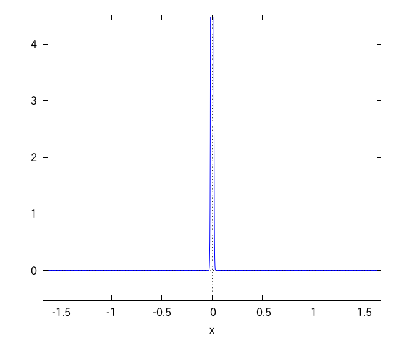
\includegraphics[keepaspectratio, width=6.5cm,height=6cm,clip]{Dirac_Delta_function3.pdf}
                        \caption{ディラックの $\delta$ 関数(1次元)の形}
                        \label{fig:delta_f2}
                    \end{center}
                \end{figure}

                        作り方は簡単.まず,面積1のグラフを用意する(図\ref{fig:delta_f24}).
                \begin{figure}[hbt]
                    \begin{center}
                        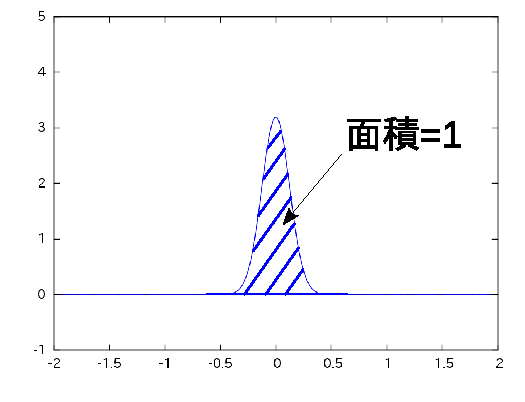
\includegraphics[keepaspectratio, width=6.5cm,height=6cm,clip]{Dirac_Delta_function5.pdf}
                        \caption{ディラックの $\delta$ 関数の作り方1}
                        \label{fig:delta_f24}
                    \end{center}
                \end{figure}

                        そして,面積1を保ちながら無限に細くしていく(図\ref{fig:delta_f33}).
                \begin{figure}[hbt]
                    \begin{center}
                        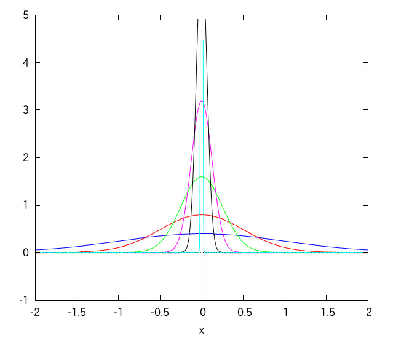
\includegraphics[keepaspectratio, width=6.5cm,height=6cm,clip]{Dirac_Delta_function4.pdf}
                        \caption{ディラックの $\delta$ 関数の作り方2}
                        \label{fig:delta_f33}
                    \end{center}
                \end{figure}
                        これで,面積が1で関数値が無限になる関数を作ることができた.

            $\delta$ 関数には次元があり,[$x^{-1}$] である.次元を持っていることを忘れやすいので,要注意.

                        ついでに,2次元の $\delta$ 関数のグラフも書いておこう.は図\ref{fig:delta_f66}下の通り.
                \begin{figure}[hbt]
                    \begin{center}
                        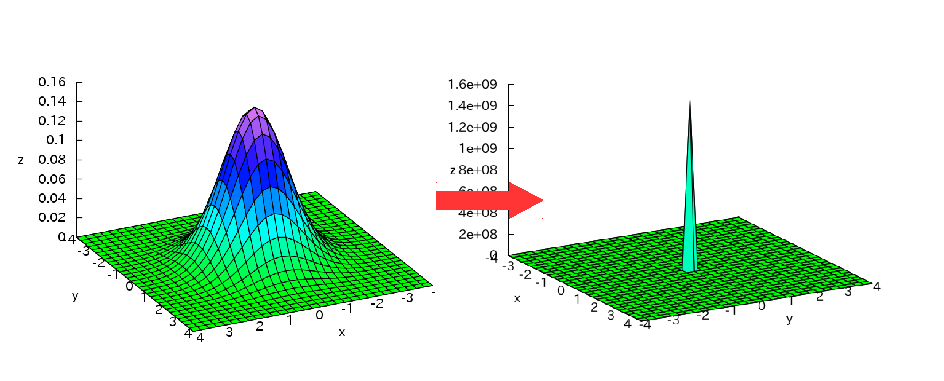
\includegraphics[keepaspectratio, width=6.5cm,height=6cm,clip]{Dirac_Delta_function6.pdf}
                        \caption{ディラックの $\delta$ 関数(2次元)の形}
                        \label{fig:delta_f66}
                    \end{center}
                \end{figure}

                        残念ながら,現実世界である3次元の $\delta$ 関数は図には描けない...

%======================================================================
%  Section
%======================================================================
\section{電流}
%======================================================================
%  SubSection
%======================================================================
    \subsection{電流のイメージ}
    おそらく,電流は説明するまでもないだろう.電気の流れのことである.い
    ままでの言葉を使えば,\textbf{電流} とは電荷の運動のことである,とい
    えよう.観測者Aに対して,荷電粒子が速度を持って運動しているとき,観測
    者Aは荷電粒子を見て,「電流が生じている」と認識するのである.この運動
    する荷電粒子は,一般に,数え切れないほど多くの数であることを想定する
    場合が多い.特に断りのない限り,電流とは,多数の荷電粒子の運動である.

    電気回路に流れる電流も多数の荷電粒子の流れであるが,この荷電粒子は導
    線中を移動することしかできない.そこでここでは,もう少し電流のイメー
    ジを拡張して,任意の空間に流れる電流を認めよう.荷電粒子は導線内部に
    しか存在できないわけではない.真空中に存在することもある.電流は導線
    だけに流れるものではない.

    電流を記号で表すときには,$I$ を用いることが多い.

    電気回路での電流のイメージは図\ref{fig:EM_Denryu01}(A)のようになろう.
    導線の中の電子をイメージしたら,図\ref{fig:EM_Denryu01}(B)の様になるかもしれない.
    しかし,実は図\ref{fig:EM_Denryu01}(B)のイメージは物性物理学的に間違っている.
    実際の電流の発生機構を説明するには原子の構造の解明や量子力学の知識が必要であり,
    それをここで考えることはできない.
    しかし,電磁気学では電荷の流れ方がどのようになっているかは説明できない.
    それとは関係なしに理論が成立している.

    電磁気学での電流とは電荷の移動であり,その場所は問われていない(導線内部である必要はない).
        具体的イメージも大事だが,ここではそれにとらわれず,抽象的な電流を考えるべきである.
        何度も言うが,電流とは空間中を移動する電荷のことである.どのように移動するかは別問題である.
        そうした抽象的な電流を考えるならば,図\ref{fig:EM_Denryu01}(B)のイメージは,
        荷電粒子の通り道を任意の空間と捉えることで,正しいイメージとなる.
        \begin{figure}[hbt]
            \begin{tabular}{cc}
                \begin{minipage}{0.5\hsize}
                    \begin{center}
                        \includegraphicsdouble{EM_Denryu01.pdf}

                        (A) 電気回路
                    \end{center}
                \end{minipage}
                \begin{minipage}{0.5\hsize}
                    \begin{center}
                        \includegraphicsdouble{EM_Denryu02.pdf}

                        (B) 一般化
                    \end{center}
                \end{minipage}
            \end{tabular}
            \caption{電流(イメージ)}
            \label{fig:EM_Denryu01}
        \end{figure}



%======================================================================
%  SubSection
%======================================================================
    \subsection{電流の定義(仮)}
        電流を数式を用いて定義しておこう.電流とは多数の点電荷の集まりの平均的な移動
        のことである.この移動を畏まった言い方をすると,次のように言える.

        ここに電流の通り道(導線)があるとしよう.
        このとき,電流を次のように定義する.
        \\
        \begin{itembox}[l]{\textbf{電流の定義(仮)}}
            \begin{itemize}
                \item 電流とは,導線の断面を単位時間1[s]に通過する
                      電荷の量を,\textbf{電流} という
                \item 電流の単位は[A]という記号で表される
                \item 電荷の単位はクーロン([C])であるので,電流の単位[A]は
                      [A]$=$[C/s]という関係がある
                \item 電流を表す標準的な記号として,このノートでは,$I$,
                      もしくは,$i$ を用いることにする
                        \footnote{
                            記号 $i$ は数学では虚数単位として用いられる
                            記号であるが,物理学や工学では電流を表すことに
                            用いることが多い(その方が一般的).なので,
                            物理学では虚数単位として,$j$ が採用されている.
                            $i$ の次のアルファベットだからだろうか.おそらく,
                            特別の意味などはないはず.文字の意味に注意しよう.
                        }
            \end{itemize}
        \end{itembox}
        \\
        \begin{figure}[hbt]
            \begin{center}
                \includegraphicslarge{EM_Denryu.pdf}
                \caption{電流(イメージ)}
                \label{fig:EM_Denryu}
            \end{center}
        \end{figure}

    \begin{memo}{注意}
        実は,この電流の単位は現在では採用されていない.
        正式な単位の定義は,後に必要な知識を説明した上で行う.
        電流に単位がないと,電流に関する事柄を扱いにくいので,
        ここではとりあえず,最も直感的で自然な定義を説明した.
        この節で「(仮)」と表現しているのは,このことによる.
    \end{memo}

%======================================================================
%  SubSection
%======================================================================
    \subsection{電流密度}
    電流とは,導線の垂直断面を,一秒間に流れる電気量として定義した.
    さらにここで,単位断面積1[m${}^{2}$]を単位時間1[s]の間に,
    どのくらいの電流が生じるかを示す \textbf{電流密度} を定義する
        \footnote{
            注意しておこう.電流密度の“密度”とは,単位面積当たりの
            密度のことである.電荷密度では,単位体積当たりの密度のこ
            とであり,両者(電荷密度と電流密度)の“密度”という語彙
            の違いは区別しておく必要がある.(次元解析をしていて,これ
            らの単位を混同してしまって,頭が混乱してしまったことがあ
            る.時間の無駄であった.)
        }.

        導線に生じている電流 $I$ が,いかなる場合でも,一様で
            \footnote{
                一様に:“むらなく”とか,“偏りなく”といった意味で使用される語彙.
            }
        あるならば,電流密度を導入することは無駄である.しかし,
        現実には,導線に生じる電流は一様ではなく,ある部分に集中的に多く
        流れていたり,ある部分には電荷の流れが全くないこともある.たしかに
        導線全体を見渡した正味の電流は一定値をとっているが,その導線の内部
        を詳細に見ることができるならば,電流にむらがあることを知るだろう.

        電流密度を $\bi(\br)$ と表す.単位は[A/m${}^{2}$]である
            \footnote{
                電荷密度 $\rho$ の単位 [C/m${}^{3}$]との違いに注意.
                電流密度は単位面積当たりの量で,電荷密度は単位体積当たり
                の量である.
            }.
        \begin{figure}[hbt]
            \begin{center}
                \includegraphicslarge{EM_DenryuMitsudo1.pdf}
                \caption{電流密度(イメージ)}
                \label{fig:EM_DenryuMitsudo1}
            \end{center}
        \end{figure}

%======================================================================
%  SubSection
%======================================================================
    \subsection{電流密度と電流の関係}
        電流 $\bI$ と電流密度 $\bi$ の関係を示そう.
        まず,電流の大きさ $I=|\bI|$ と電流密度 $\bi(\br)$ の関係を考える.

        導線の断面を $S_{l}$ とし,また,
        その一部の微小断面を $\df S_{l}$ とする
            \footnote{
                添字の $l$ は曲面 $S_{l}$ の縁となる閉曲線を表す.
                一般に,曲面は縁があるはずで,その縁は閉曲線である.
            }.
        この微小断面 $\df S_{l}$ の単位法線ベクトルを $\bn(\br)$ とかこう.

        このとき,電流密度 $\bi(\br)$ の微小断面 $\df S_{l}$ の垂直成分は
            \begin{align*}
                \bi(\br) \cdot \bn(\br) \df S_{l}
            \end{align*}
        で表現できる.そして,これを全断面 $S$ で面積分した値は,
        電流の大きさ $I$ に等しい.すなわち,
            \begin{align*}
                I = \sint_{S_{l}}\bi(\br) \cdot \bn(\br) \df S_{l}.
            \end{align*}

        まとめておこう.
        \begin{myshadebox}{電流密度と電流の関係}
            閉曲線 $l$ を縁とする曲面 $S_{l}$ を貫く電流 $I$ と,
            電流密度 $\bi(\br)$ の関係は,次式で表される.
            \begin{align}
                I = \sint_{S_{l}}\bi(\br) \cdot \bn(\br) \df S_{l}.
            \end{align}
            ここに,$\bn(\br)$ は $S_{l}$における各微小部分 $\df S_{l}$ の
            単位法線ベクトルである.
        \end{myshadebox}

        \begin{figure}[hbt]
            \begin{center}
                \includegraphicslarge{LI_si_00.pdf}
                \caption{電流と電流密度}
                \label{fig:LI_si_00}
            \end{center}
        \end{figure}

    \begin{memo}{微小面積と単位法線ベクトル}
        微小面積とは,全面積 $S$ の微小な一部分のことである.
        また,単位法線ベクトルとは,面に垂直方向で長さが1のベクトルのことである.
        \begin{figure}[hbt]
            \begin{center}
                \includegraphicslarge{EM_smollS.pdf}
                \caption{微小体積}
                \label{fig:EM_smollS}
            \end{center}
        \end{figure}
    \end{memo}

    \begin{memo}{面積分の表示方法}
        面積分は,2方向にわたる積分である.
        つまり,2つの積分変数 $u$,$v$ を
        考えたとき,これを変数に持つ関数 $f(u,\,v)$ をとし,
            \begin{align*}
                \int \left( \int f(u,\,v) \df u \right) \df v
            \end{align*}
        を計算することが,面積分を行うということである.

        つまり,$f(u,\,v)$ を最初に $u$ について積分して,その結果をさらに,
        $v$ について積分するということである.計算方法を示すには,このような
        表示の仕方が有効であるが,この表現からでは面積分であることをイメージする
        には,少々難しい.そこで,式を次ように書き換えてみる.
            \begin{align*}
                 \sint f(u,\,v) \df u \df v
            \end{align*}
        括弧をなくしただけである.そして,
        $\df S := \df u\df v$ という量を導入し,
        さらに,2回の積分を改て $\sint_{S}$ と表現することで,
            \begin{align*}
                \sint_{S} f(u,\,v) \df S
            \end{align*}
        となる.これならば,面 $S$ で面積分するというイメージが
        しやすい式の表現になった.

        ちなみに,$\df S := \df u\df v$ は \textbf{面積素} とよばれる.
    \end{memo}



%   %-----------------------------------------------------------------------------------------------
%   %  Input
%   %    File Name : PhysNote_EM_1st_RShipIandRho.tex
%   %    説明      : 電流と電荷の関係を説明する.
%   %-----------------------------------------------------------------------------------------------
        %===================================================================================================
%  Chapter : 電磁気学の基本概念
%  説明    : 電荷の存在や,電流の存在などを確認する
%===================================================================================================
%======================================================================
%  Section
%======================================================================
\section{電流と電荷の関係}
\begin{mycomment}
    \textbf{電荷} とは,電磁気現象の発生原因であり,この存在は有無をいわさず
    受け入れさせられるものである.\textbf{電流} とは,一つ,あるいは複数(多数)の
    電荷が,平均的に一方向に移動しているような現象をいう.従って,
    電流とは,電荷と観測者の相対的な速度に依存していると考えられる.つまり,
    観測者が電荷を見ているとき,その観測者の速度により,電流が生じているのか,
    単に電荷が運動せずにその場に存在しているのかが,変わってきてしまう.
    そこで,以降では,観測者の速度を0として,扱うことにする.
\end{mycomment}
%======================================================================
%  SubSection
%======================================================================
    \subsection{大局的な電荷保存則}
        \begin{mysmallsec}{電荷は突然現れることはない}
        ある領域に電荷が多数存在していることを想定しよう(図\ref{fig:Denryu_Denka_intoro}(A)参照).
        この多数の電荷の電気量の総和を,$Q(t)$ と書くことにする
            \footnote{
                電荷が多数存在するが,その個数は有限であることを想定する.
                このとき,電荷に番号付けをして,$q_{0}$,$q_{1}$,$q_{2}$,$\cdots$ の
                ように書けば,その総和 $Q(t)$ は $Q(t):=\sum_{i}^{N(t)}q_{i}$ で表せる.
                左辺の総電気量 $Q(t)$ の独立変数 $t$ は,右辺の電荷の個数が時間変化する場合($N(t)$)を
                表したものである.
            }.
        この状態から,ある程度時間が経過して,領域内部の電気量の総和が変化したとしよう.
        つまり,$Q$ の時間微分が0ではない値をとるということになる
            \footnote{
                時間変化がないということは,時間微分して0であるということである.
                例えば,速さ $v(t)$ は $v(t):=\df x(t)/\df t$($x$ は位置,$t$ は時間を表す)で
                定義されるが,位置に時間変化がない場合 $x(t)$ は一点に止まっているので,
                $x(t)=X_{\mathrm{const}}$ となり,時間によらない定数 $X_{\mathrm{const}}$ で表せる.
                この時の速度を考えると,$v(t):=\df x(t)/\df t=\df X_{\mathrm{const}}/\df t = 0$ と
                なり,位置の時間微分は0である.つまり,位置が時間変化しない(動かない)物体の
                一の時間微分は0になる.これは逆に,位置の時間微分が0であれば,
                その物体は動いていない,と言うこともできる.さらに,物体の位置の時間微分が0でない値
                を取るならば,その物体は動いていると言える.

                今回の場合,時間変化するのは領域内の総電気量 $Q(t)$ である.
            }.
        総電気量が変化したということは,その領域内部の電荷の量が変化したということである.
        つまり,個々の電荷が領域外部に出て行ったり,あるいは逆に,領域外部から電荷が入ってきた
        ということである.すなわち,
            \begin{equation*}
                \frac{\df Q(t)}{\df t} \neq 0.
            \end{equation*}
        ここで,出たり入ったりする電荷の,正味の電気量を $I(t)$ と書けば,
            \footnote{
                ここで記号として $I(t)$ を書いたのは,電流 $I(t)$をあとで定義する
                ためである.独立変数として,時間 $t$ を明示したのは,時刻によって
                生じる電流が,異なる場合を想定したからである.
            },
            \begin{equation*}
                \frac{\df Q(t)}{\df t} + I(t) = 0.
            \end{equation*}
        となるような $I(t)$ が存在することになる.要は,領域内部の総電気量 $Q(t)$ の
        時間変化に,正味の電荷の出入り $I(t)$ を足し合わせれば0であるということである.
        もっと簡単に言うと,領域内部の総電気量の変化は,外部との電荷のやり取りで
        生じるのであり,その領域内部でいきなり電荷が現れたり消えたりしない,という
        ことである(図\ref{fig:Denryu_Denka_intoro}(B)参照).この電荷の出入りを表す $I(t)$ が
        電流である.端的に言えば,ある領域内の総電気量が変化したことと,その領域に電流が生じ
        ていることとは,等価である.
        \end{mysmallsec}

        \begin{mysmallsec}{電荷保存の法則}
        実は,この考え方こそが,\textbf{電荷保存の法則} であり
            \footnote{
                略して,\textbf{電荷保存則} といわれることのほうが,一般的である.
            },今の場合は,
        \textbf{大域的(マクロ)な}視点から見た電荷保存則(脚注参照)である.後ほど,一般化して,
        \textbf{局所的な}電荷保存則も紹介することになる.

        改めて,大局的な電荷保存則を記述しておこう.
            \begin{myshadebox}{(大局的な)電荷保存則}
                ある領域内部の総電気量を $Q(t)$ とし,その内部から外部へ向かって電流 $I(t)$ が
                生じている場合,
                \begin{align}
                    \frac{\df Q(t)}{\df t} = - I(t).
                \end{align}
                という関係式が成立する.これを,
                大局的な \textbf{電荷保存の法則}(あるいは略して,\textbf{電荷保存則})という.
            \end{myshadebox}

        ここで,電流 $I(t)$ を右辺に移項した.この表現の方が,総電気量の時間変化と
        電流が等価であることを,イメージしやすいからである.また,多くの教科書で,
        この書き方がなされている.電流の符号は,領域内の総電気量が減る場合には正
        (電荷が領域内部から飛び出して,それが電流となる),
        領域内の総電気量が増える場合には負(領域内に電流が入ってきて,内部の電荷個数が増える)とする
            \footnote{
                簡単に言うと,領域から電流が外向きに生じているときに正,
                領域に電流が吸収される場合に負とする.
            }.
        \end{mysmallsec}
                \begin{figure}[hbt]
                    \begin{tabular}{cc}
                        \begin{minipage}{0.5\hsize}
                            \begin{center}
                                \includegraphicsdouble{Denryu_Denka_intoro001.pdf}

                                (A) 領域内の電荷
                            \end{center}
                        \end{minipage}
                        \begin{minipage}{0.5\hsize}
                            \begin{center}
                                \includegraphicsdouble{Denryu_Denka_intoro002.pdf}

                                (B) 電荷の出入り
                            \end{center}
                        \end{minipage}
                    \end{tabular}
                        \caption{電流と電荷}
                        \label{fig:Denryu_Denka_intoro}
                \end{figure}

%======================================================================
%  SubSection
%======================================================================
    \subsection{局所的な電荷保存則}
        電荷保存則は,局所的にも成立する法則である.理論物理学では,
        大局的表現よりも,これから説明する局所的な電荷保存則の表現
        がよく使われる.大局的な表現がすでに得られているので,そこ
        から,局所的表現を導出しよう.

        まず,電流 $I(t)$ と総電気量 $Q(t)$ を,それぞれ電流密度 $\bi$ と
        電荷密度 $\rho$ で書きなおしておこう.
            \begin{align*}
                I(t)  &=  \sint_{S} \bi \cdot \bn \df S. \\
                Q(t)  &=  \vint_{\Omega_{S}} \rho \df V.
            \end{align*}
        電流道度 $\bi$ と電荷密度 $\rho$ は,位置と時間の関数であることに注意.
            \begin{equation*}
                \bi := \bi(\br,\,t)\,,\quad \rho := \rho(\br,\,t).
            \end{equation*}
        ちなみに,電流 $I(t)$ と総電気量 $Q(t)$ の独立変数に位置 $\br$ が
        ないのは,位置で積分してしまうためである
            \footnote{
                積分変数は積分後には残らない.大局的視点から見るので,
                細かな位置を知る必要はなく,この視点で重要なのは,考察範囲
                全体の電流量や電気量なのである.これから考える局所的な量は,
                その位置も重要になる.大局的視点と局所的視点の違いは意識して
                おくべきことだろう.
            }.
        電流道度 $\bi$ と電荷密度 $\rho$ を用いると,電荷保存則は次のように書ける.
            \begin{equation*}
                 \frac{\rd}{\rd t} \left( \vint_{\Omega_{S}} \rho \df V \right)
               = - \sint_{S} \bi \cdot \bn \df S.
            \end{equation*}

        ここで,上式の右辺にガウスの定理
            \footnote{
                任意のベクトル $\bX$ に対して,
                \begin{equation*}
                      \sint_{S} \bX \cdot \bn \df S
                    = \vint_{\Omega_{S}} \ddiv \bX \cdot \bn \df V.
                \end{equation*}

                後で簡単に復習するので,そこを参照のこと.
                それでもわからなければ,数学の解説の部分を
                読むこと.さらにそれでもわからなかったら,
                ベクトル解析教科書を別途お読みください.
            }
        を適用する.
            \begin{equation*}
                  \vint_{\Omega_{S}} \frac{\rd \rho}{\rd t} \df V
                = - \vint_{\Omega_{S}} \ddiv \bi \cdot \bn \df V.
            \end{equation*}
        この式変形で,左辺の空間微分と時間微分の可換性
            \footnote{
                空間に関する微分と,時間に関する微分は計算順序を入れ替えても,
                結果は変わらないということ.
            }
        を利用した.
        この式の両辺を見ると,積分範囲が同じ体積分になっている.この等式が一般的に成り立つのは,
        両辺の被積分関数が等しいときである
            \footnote{
                数学的に示すべきことだろうが,ここでは割愛する.
            }.
            \begin{equation*}
                  \frac{\rd \rho}{\rd t} = -\ddiv \bi.
            \end{equation*}
        慣習に従って,次のように書き換える.
            \begin{align}\label{eq:bisiteki_denkahozonsoku00}
                \ddiv \bi = -\frac{\rd \rho}{\rd t}.
            \end{align}
        この式(\ref{eq:bisiteki_denkahozonsoku00})が,
        局所的な \textbf{電荷保存則} である.

        ある局所的領域
            \footnote{
                局所的領域:可能なかぎり小さくした領域のこと.あくまでも,
                直感的な言葉であり,「可能なかぎり」に特別な意味は込めていない.
                日常言語的な捉え方をしてもらいたい.
            }
        から電流が湧き出る($\ddiv \bi$)ならば,その領域内部の電荷密度は
        減少する($-(\rd \rho/\rd t)$)ということを,式で表現できている.

        改めて,まとめておこう.
            \begin{myshadebox}{(局所的な)電荷保存則}
                ある局所的領域から電流が湧き出る($\ddiv \bi$)ならば,
                その領域内部の電荷密度は減少する($-\rd \rho/\rd t$).
                \begin{align}
                    \ddiv \bi = -\frac{\rd \rho}{\rd t}.
                \end{align}
                これは,電荷保存則を局所的に表現したものである.
            \end{myshadebox}

            \begin{memo}{ガウスの定理(復習)}
                ガウスの定理:ガウスの法則とは別のもの.ガウスの定理は数学上の
                              定理である.この定理により,以下の等式が成立する.

                                任意のベクトル $\bX$ に対して,
                                \begin{equation*}
                                      \sint_{S} \bX \cdot \bn \df S
                                    = \vint_{\Omega_{S}} \ddiv \bX \cdot \bn \df V.
                                \end{equation*}

                                言葉で説明するならば,次のようなイメージになろう.
                                「任意の閉曲面 $S$ で囲まれた領域 $\Omega_{S}$ より
                                湧き出る $\ddiv \bX$ の総和は,閉曲面 $S$ の表面から
                                抜け出る正味の流出量に等しい」.
            \end{memo}



%===================================================================================================
%  Chapter : クーロンの法則
%  説明    : 電磁気学の要である,電気力=クーロン力について説明する
%===================================================================================================
\chapter{クーロンの法則}
%   %-----------------------------------------------------------------------------------------------
%   %  Input
%   %    File Name : PhysNote_EM_1st_CoulombLow.tex
%   %    説明      : 電場を導入する
%   %                を説明する.
%   %-----------------------------------------------------------------------------------------------
        %===================================================================================================
%  Chapter : クーロンの法則
%  説明    : 電磁気学の要である,電気力=クーロン力について説明する
%===================================================================================================
%======================================================================
%  Section
%======================================================================
    \section{クーロン力}\label{sec:CoulomnbForce}
%   %==================================================================
%   %  Subsection
%   %==================================================================
    \subsection{法則}
        電荷を帯びた物体が受ける,電気的な力というものが,世の中に
        存在する.これは万人が知っている事実だから,ここで改めて明
        記することは,バカバカしく感じられる.しかし,この電気的な
        力の存在は,大変重要なものである.この電気的な力のことを,
        \textbf{クーロン力} とよぶ.電気量の単位であるクーロンと同
        じ名前を持っているが,お察しのとおり,同一人物に由来するも
        のである.

        クーロン(Coulomb)は,電気的な力の性質を実験的に知ることに
        成功した
            \footnote{
                電気量の定義は,クーロン力を基にしてなされるもの
                である.
            }.
        そして,クーロンは,電気的な力が,次のような性質を持っていることを
        明らかにした.
        \\
        \begin{itembox}[l]{\textbf{クーロン力(クーロンの法則)}}
            ここに,電荷が2つあるとしよう.この2つの電荷は区別する
            ことができて,$q_{1}$,$q_{2}$ という電気量を持っている
            とする.電荷 $q_{1}$ と $q_{2}$ との距離を $r$ としたと
            き,この2つの電荷が受ける力は,以下のような規則がある.
            \begin{itemize}
                \item 2つの電荷の電気量が互いに異なる符号をもってい
                      るならば,両電荷は互いに引き合う向きに力を受
                      ける
                \item 2つの電荷の電気量が同じ符号を持っているならば,
                      両電荷は互いに反発しあう向きに力を受ける.
                \item 2つの電荷の受ける力の大きさは等しく,
                      向きは互いに逆向きである
                \item 2つの電荷が受ける力の大きさは,
                      2つの電荷の電気量の積($q_{1}q_{2}$)に比例する.
                \item 2つの電荷が受ける力の大きさは,
                      2つの電荷間の距離の2乗($r^{2}$)に反比例する.
            \end{itemize}
        \end{itembox}
        \\
        \begin{figure}[hbt]
            \begin{tabular}{cc}
                \begin{minipage}{0.5\hsize}
                    \begin{center}
                        \includegraphicsdouble{coulombs_low1.pdf}

                        (A)
                    \end{center}
                \end{minipage}
                \begin{minipage}{0.5\hsize}
                    \begin{center}
                        \includegraphicsdouble{coulombs_low2.pdf}

                        (B)
                    \end{center}
                \end{minipage}
            \end{tabular}
                        \caption{クーロン力}
                        \label{fig:coulombs_low}
        \end{figure}

        上に書いたような,クーロン力が示す性質のことを,\textbf{クーロンの法則} と
        いう.これは電磁気学の最も基本的な法則であり,大変重要な法則である.
        あとに説明する \textbf{電場} という重要な概念の導入も,
        このクーロンの法則を基にしている.

        言葉で書いてしまうと,ちょっとややこしいかもしれない.
        しかし,いきなり数式を出してしまうと,それはそれで
        尻込みしてしまうので,とりあえず言葉で説明してみた.

%   %==================================================================
%   %  Subsection
%   %==================================================================
    \subsection{定量化}
        では,次の段階に進み,クーロンの法則を数式で表現してみよう.
        数式で表現すると,とても簡潔になることを感じ取ることができる
        だろう.

        図\ref{fig:Coulombs_Force}のような状態であるとしよう.
        \begin{figure}[hbt]
            \begin{center}
                \includegraphicslarge{Coulombs_Force.pdf}
                \caption{クーロンの法則}
                \label{fig:Coulombs_Force}
            \end{center}
        \end{figure}

        2つの区別可能な電荷が存在し,それぞれの電気量が,$q_{1}$,$q_{2}$ で
        あるとする.また今後,これらの電荷自体を表現する場合にも,
        「電荷 $q_{1}$」などのように記述する
            \footnote{
                同じ記号に二つの意味を込めるのはよくないが,
                そうかと言って,無嫌味に記号を増やして読みづらくしたくも
                ない.ここでは,誤解を生むことがないと判断し,同じ記号で
                “電荷それ自体”と“その電気量”の2つを同じ記号で表すこと
                とする.
            }.
        この2つの電荷がある位置を,それぞれ $\br_{1}$,$\br_{2}$ と
        する.このとき,電荷間の距離 $r$ は,
            \begin{equation*}
                r = | \br_{2} - \br_{1} |.
            \end{equation*}
        また,電荷 $q_{2}$ から見た,電荷 $q_{1}$ の位置 $\br_{12}$は,
            \begin{equation*}
                \br_{12} = \br_{1} - \br_{2}.
            \end{equation*}
        同様に,電荷 $q_{1}$ から見た,電荷 $q_{2}$ の位置 $\br_{21}$は,
            \begin{equation*}
                \br_{21} = \br_{2} - \br_{1}.
            \end{equation*}

        「2つの電荷が受ける力は,大きさが同じで,向きが逆である.」これを
        数式で表すには,まず,大きさと向きを文字で表現すべきだ.
        同時に考えるのは難しいので,まずはクーロン力の大きさだけを考える.
        電荷 $q_{1}$ が受けるクーロン力 $F_{12}$ は,
        2点電荷の電気量の積 $q_{1}q_{2}$ に比例するので,数式的には,
            \begin{equation*}
                F_{12} = \alpha q_{1}q_{2}
            \end{equation*}
        とかける.ここに,$\alpha$ 比例定数である
            \footnote{
                この比例定数 $\alpha$ には全く意味が無い.単に
                比例を表すのに,便宜的に使ったに過ぎない.
                同じことがすぐ後に使う,$\beta$ についても言える.
                しかし,最後に現れる比例定数 $k$ については,
                重要であるので注意すべきだ.
            }.
         また同時に,
        「2つの電荷が受ける力の大きさは,2つの電荷間の距離の
        2乗($r^{2}$)に反比例する」から,
            \begin{equation*}
                F_{12} = \beta \frac{1}{r^{2}}
            \end{equation*}
        ともかける.$\beta$ も比例定数である.
        この2つの $F_{12}$ の式は矛盾なく両立する.
        この2つの式をまとめて,
            \begin{equation*}
                F_{12} = \alpha \beta \frac{q_{1}q_{2}}{r^{2}}
            \end{equation*}
        となる.ここで,式の見易さのため,比例定数 $\alpha \beta$ を
        改めて $k$ とおいて($k=\alpha \beta$),
            \begin{align}\label{eq:coulomb_force_f1_ookisa}
                F_{12} = k \frac{q_{1}q_{2}}{r^{2}}
            \end{align}
        とすれば,この式(\ref{eq:coulomb_force_f1_ookisa})によって,
        電荷 $q_{1}$ が受けるクーロン力の大きさを
        記述できたことになる.

        残りはその方向であるが,これは簡単だ.単位ベクトルを考えれば
        よい.一般のベクトル $\bA$ に対する単位ベクトルとは,大きさが $1$ で,
        その方向が $\bA$ と同じ向きのようなものである.このような単位ベクトルが
        存在したとして,$\bn$ と表そう.この時,$\bA$ は,$\bA=|\bA|\bn$ と書き
        表せる.つまり,単位ベクトル $\bn$ について解けば,
            \begin{equation*}
                \bn = \frac{\bA}{|\bA|}
            \end{equation*}
        である.

        今の場合に当てはめて考えれば,$\bA=\br_{12}$ であるから,
        単位ベクトルは
            \begin{equation*}
                \bn = \frac{\br_{12}}{|\br_{12}|}
                    = \frac{\br_{1} - \br_{2}}{|\br_{1} - \br_{2}|}
            \end{equation*}
        である.これが,電荷 $q_{1}$ が受けるクーロン力の向きを
        表している.

        これで,電荷 $q_{1}$ の受けるクーロン力の大きさと向きの
        数式的表現を,別々ではあるが,表現できた.あとは
        この2つを一緒に表せれば,完了となる.

        ここで改めて,電荷 $q_{1}$ の受ける
        クーロン力を向きも考慮して $\bF_{12}$ と表すこととすると,
        $\bF_{12}$ は,その大きさ $F_{12}$ と単位ベクトル $\bn$ を
        用いて,
            \begin{equation*}
                \bF_{12} = F_{1}\bn
            \end{equation*}
        とかける.
        これに,上で得た結果を代入すればよい.すると,
            \begin{align}\label{eq:coulomb_force_f1}
                \bF_{12} = k \frac{q_{1}q_{2}}{r^{2}} \frac{\br_{1} - \br_{2}}{|\br_{1} - \br_{2}|}
            \end{align}
        となる.この式(\ref{eq:coulomb_force_f1})が目標としていた,
        電荷 $q_{1}$ が受けるクーロン力 $\bF_{12}$を,
        式で表したものである.

        これ同様に,電荷 $q_{2}$ が受けるクーロン力 $\bF_{2}$を考えること
        ができるが,「2つの電荷の受ける力の大きさは等しく,向きは互いに逆
        向きである」ということを考慮すれば,直ちに,次式を得る.
            \begin{align*}
                \bF_{21} &= - \bF_{12} \\
                        &= - k \frac{q_{1}q_{2}}{r^{2}} \frac{\br_{1} - \br_{2}}{|\br_{1} - \br_{2}|}.
            \end{align*}
        ここで,
            \begin{align*}
                -(\br_{1} - \br_{2}) &= \br_{2} - \br_{1} \\
                |\br_{1} - \br_{2}|  &= |\br_{2} - \br_{1}| \\
                q_{1}q_{2}           &= q_{2}q_{1}
            \end{align*}
        であることに気付けば
            \footnote{
                数式を見れば当たり前のように感じるかもしれないが,重要な式である.というのも,
                この関係式は作用反作用の法則を表す数式にほかならないからである.
            },
            \begin{align}\label{eq:coulomb_force_f2}
                \bF_{21} = k \frac{q_{2}q_{1}}{r^{2}} \frac{\br_{2} - \br_{1}}{|\br_{2} - \br_{1}|}
            \end{align}
        となる.$\bF_{12}$ の式(\ref{eq:coulomb_force_f1}) と比較すると,
        添字の1と2が逆になっているだけであることに気づくだろう.

        最後に,比例定数 $k$ について記述しよう.
        この比例定数は,基準とする単位系によって値は
        変化するが,今日一般的に使用されているSI単位系を
        採用するならば,
            \begin{align}
                k = \frac{1}{4\pi\varepsilon_{0}} = 8.989 \times 10^{9}
            \end{align}
        である.$\varepsilon_{0}$ は真空の \textbf{誘電率} と言われる
        物理定数であるが,これについての解説は後回しにする.
        また,$\pi$ は円周率である.

%   %==================================================================
%   %  Subsection
%   %==================================================================
    \subsection{まとめ}
        以上の計算より得た結果をまとめよう.
        \begin{myshadebox}{クーロン力}
            ある空間に2つの電荷 $q_{1}$,$q_{2}$ が,それぞれ
            位置 $\br_{1}$,$\br_{2}$ に
            存在するとき,この2つの電荷には,次式で
            表されるような力が作用する.この力のこと
            を \textbf{クーロン力} という.

            電荷 $q_{1}$ に対して働く力は以下.
               \begin{align}
                   \bF_{12} =
                       \frac{1}{4\pi\varepsilon_{0}} \frac{q_{1}q_{2}}{r^{2}}
                           \frac{\br_{1} - \br_{2}}{|\br_{1} - \br_{2}|}.
               \end{align}

        ここに,$\varepsilon_{0}$ は真空の誘電率
           \footnote{
               詳細は後述.
           }
        である.
        \end{myshadebox}


        電荷 $q_{2}$ に対しては,以下の力が働く.
           \begin{align}
               \bF_{12} = -\bF_{21} =
                   \frac{1}{4\pi\varepsilon_{0}} \frac{q_{2}q_{1}}{r^{2}}
                       \frac{\br_{2} - \br_{1}}{|\br_{2} - \br_{1}|}.
           \end{align}


    \begin{memo}{(例)2つの点電荷同士のクーロン力}
    クーロンの法則を,より感覚的に分かるように,ここで,
    最も簡単な,2つの点電荷間に働く,クーロン力を考てみよう.

    存在する電荷が点電荷の場合,クーロンの法則は次式で表せる.
            \begin{align}
                \bF_{12}=\frac{1}{4\pi\varepsilon_{0}}
                \frac{q_{1}q_{2}}{|\br_{1}-\br_{2}|^{2}}
                \frac{\br_{1}-\br_{2}}
                     {|\br_{1}-\br_{2}|}.
            \end{align}
    より考えやすくするために,2次元で考えてみよう.座標系は,直交座標系とする.
    この場合,
        \begin{equation*}
            |\br_{1}-\br_{2}| = \sqrt{ {\left(x_{2} - x_{1}\right)}^{2}
            + {\left(y_{2} - y_{1}\right)}^{2} }
        \end{equation*}
    である.
        \begin{figure}[hbt]
            \begin{center}
                \includegraphicslarge{2point_distance.pdf}
                \caption{一般の2つの点の間の距離}
                \label{fig:2point_distance}
            \end{center}
        \end{figure}


    点電荷の配置を,$x$ 軸上にし,各電荷が $x=-1/2$,$x=1/2$ に存在しているとする.
    そうすると,2つの点電荷のそれぞれの位置ベクトルは,
    $\br_{1}  =  ( \,-1/2\,,\,0\, )$,$\br_{2}  =  ( \,1/2\,,\,0\, )$ となる.
    そうすると,
            \begin{align*}
                |\br_{1}-\br_{2}|
                &= \sqrt{ {\left(x_{2} - x_{1}\right)}^{2} + {\left(y_{2} - y_{1}\right)}^{2} } \\
                &= \sqrt{ {\left(\frac{1}{2} - \left(-\frac{1}{2}\right)\right)}^{2} + {\left(0-0\right)}^{2} } \\
                &= 1.
            \end{align*}
    電荷量の
    大きさは,両電荷ともに等しく,$1$[C] として考える.
        \begin{figure}[hbt]
            \begin{center}
                \includegraphicslarge{example_Coulombs_low1.pdf}
                \caption{例:2つの点電荷間のクーロン力}
                \label{fig:example_Coulombs_low1}
            \end{center}
        \end{figure}

    すると,クーロンの法則は,次のようになる.電荷 $q_{1}$ が,電荷 $q_{2}$ から
    受けるクーロン力 $\bF_{12}$ は
            \begin{align*}
                \bF_{12}
                &= \frac{1}{4\pi\varepsilon_{0}}
                \frac{q_{1}q_{2}}{|\br_{1}-\br_{2}|^{2}}
                \frac{\br_{1}-\br_{2}}
                     {|\br_{1}-\br_{2}|} \\
                &= \frac{1}{4\pi\varepsilon_{0}}
                \frac{1}{ 1 }
                \frac{\left( \,-1\,,\,0\, \right)}
                     { 1 } \\
                &= \frac{1}{4\pi\varepsilon_{0}} \left( \,-1\,,\,0\, \right)
            \end{align*}
    と書ける.

    クーロン力の向きは,$\left( \,-1\,,0\,\right)$ であることが
    分かった.

    以下では,クーロン力の大きさのみ($| \bF_{12} | := F_{12}$)を考えていこう.
        \begin{align*}
            |\bF_{12}|  &= F_{12} \\
                        &= \frac{1}{4\pi\varepsilon_{0}} \sqrt{(-1)^{2}+0^{2}} \\
                        &= \frac{1}{4\pi\varepsilon_{0}} \cdot 1               \\
                        &= \frac{1}{4\pi\varepsilon_{0}}
        \end{align*}

    最後に,$\varepsilon_{0}$,$\pi$ に具体的な数値を代入する.
    ここではとりあえず,
        \begin{equation*}
            \varepsilon_{0} = 8.854 \times 10^{-12}
        \end{equation*}
    であることが知られているので,この数値を使うことにする.
    しかし,どのようにして,このような数値が分かるかについては,
    後ほど,電磁気学をさらに学んでから,考えなおすことにしたい.
    $\pi$ は周知のように,
        \begin{equation*}
            \pi = 3.141
        \end{equation*}
    である.

    以上から,
            \begin{align*}
                F_{12}
                &= \frac{1}{4\pi\varepsilon_{0}} \\
                &= \frac{1}{4 \times 3.1415 \times 8.854 \times 10^{-12}} \\
                &= \frac{10^{12}}{ 222.483 }  \\
                &= 0.008989 \times 10^{12}  \\
                \therefore\quad
                F_{12}
                &= 8.989 \times 10^{9}
            \end{align*}
    を得る.

    実は,今までの計算は,単位電荷1[C]をもつ2つの点電荷が,1[m]離れて位置する
    場合のクーロン力を計算していた.つまり,
        \begin{equation*}
            \frac{q_{1}q_{2}}{r^{2}} = 1
        \end{equation*}
    となるのは,あたり前のことであった.しかし,
    あえて,座標から丁寧に計算したのは,点電荷がどのような位置に存在しても,
    同じように計算できることを,示したかったからである
        \footnote{
            この例はとても簡単だが,一般性が高い理論であることを認識
            することはできるはず.
        }.

    上の計算から,
        \begin{align}
            \frac{1}{4\varepsilon_{0} \pi} \simeq 9.0 \times 10^{9}
        \end{align}
    が分かる.この数値を用いて,クーロン力を表すと,
        \begin{align}
            F = 9.0 \times 10^{9} \times \frac{q_{1}q_{2}}{r^{2}}
        \end{align}
    となる.

    高校物理では,$k=9.0 \times 10^{9}$ と置いて,
        \begin{equation*}
            F = k \frac{q_{1}q_{2}}{r^{2}}
        \end{equation*}
    と書かれることも多い.
\end{memo}

%======================================================================
%  Section
%======================================================================
    \section{力の重ねあわせの原理}
        クーロン力は,力学的な力と同様に,重ねあわせの原理が成立
        していることが,実験的に確認されている.

        具体例で示したほうが,分かりやすい.
        3つの点電荷が存在する場合を考える.
        \begin{figure}[hbt]
            \begin{center}
                \includegraphicslarge{EM_Coulomb_KasaneAwase01.pdf}
                \caption{クーロン力(3つの点電荷)}
                \label{fig:EM_Coulomb_KasaneAwase00}
            \end{center}
        \end{figure}

        電気量 $q_{1}$,$q_{2}$,$q_{3}$ をもつ3つの点電荷
        の内,任意に2つを選ぶ.ここでは $q_{1}$ と $q_{2}$ をえらぼう.
        ここでは,例として,点電荷 $q_{1}$ が,他の点電荷 $q_{2}$ と $q_{3}$ から受ける
        クーロン力 $\bF_{1}$ を計算する.
        計算方法は,最初に点電荷 $q_{2}$ から受けるクーロン力 $\bldf_{12}$ を
        計算する.この時,$q_{3}$ はとりあえず存在しないとして考える
        (図\ref{fig:EM_Coulomb_KasaneAwase02}(A)).
            \begin{equation*}
                \bldf_{12} = \frac{1}{4\pi\varepsilon_{0}}
                           \frac{q_{2}q_{1}}{{|\br_{1} - \br_{2}|}^{2}}
                           \frac{\br_{1} - \br_{2}}{|\br_{1} - \br_{2}|}.
            \end{equation*}
        その次に,点電荷 $q_{3}$ から受けるクーロン力 $\bldf_{13}$ を
        計算する.この時,$q_{2}$ はとりあえず存在しないとして考える
        (図\ref{fig:EM_Coulomb_KasaneAwase02}(B)).
            \begin{equation*}
                \bldf_{13} = \frac{1}{4\pi\varepsilon_{0}}
                           \frac{q_{3}q_{1}}{{|\br_{1} - \br_{3}|}^{2}}
                           \frac{\br_{1} - \br_{3}}{|\br_{1} - \br_{3}|}.
            \end{equation*}
        \begin{figure}[hbt]
            \begin{tabular}{cc}
                \begin{minipage}{0.5\hsize}
                    \begin{center}
                        \includegraphicsdouble{EM_Coulomb_KasaneAwase02a.pdf}

                        (A)
                    \end{center}
                \end{minipage}
                \begin{minipage}{0.5\hsize}
                    \begin{center}
                        \includegraphicsdouble{EM_Coulomb_KasaneAwase02b.pdf}

                        (B)
                    \end{center}
                \end{minipage}
            \end{tabular}
            \caption{重ねあわせの原理(クーロン力)}
            \label{fig:EM_Coulomb_KasaneAwase02}
        \end{figure}

        最後に,今得た $\bldf_{12}$ と $\bldf_{13}$ を足し合わせれば,
        $\bF_{1}$ を得る(図\ref{fig:EM_Coulomb_KasaneAwase03}).
        \begin{align}
            \bF_{1} &=  \bldf_{12} + \bldf_{13}
        \end{align}
        \begin{figure}[hbt]
            \begin{center}
                \includegraphicslarge{EM_Coulomb_KasaneAwase03.pdf}
                \caption{クーロン力の重ねあわせの結果(3つの点電荷)}
                \label{fig:EM_Coulomb_KasaneAwase03}
            \end{center}
        \end{figure}

        同様に,
        \begin{align*}
            \bF_{2} &= \bldf_{21} + \bldf_{23}. \\
            \bF_{3} &= \bldf_{31} + \bldf_{32}.
        \end{align*}


%======================================================================
%  Section
%======================================================================
    \section{クーロンの法則($N$個の点電荷)}
    まず,一般的に表現する方法についての,説明する.

    いま,3つの電荷 $q_{1}$,$q_{2}$,$q_{3}$ について考えたが,
    一般的に表現したい場合には,点電荷の個数を具体的な自然数で
    表現することはできない.そこで,任意の自然数を表す記号 $N$ を
    用意する.

    さて,$N$ 個ある点電荷のうちで着目したい1つの点電荷を指したい
    場合を考える.この場合,あらかじめ $N$ 個の点電荷に番号付けを
    しておく.その上で,例えば「番号1の点電荷に着目して$\cdots$」な
    どといえば,特定の点電荷に着目できる.しかし,全ての電荷につい
    て一度に当てはまる一般的な性質を議論するときには,具体的な番号
    を指定して一つずつ議論するのは,とても効率が悪い
        \footnote{
            $N$ 個の電荷について,すべて同じ議論を繰り返すことになる.
        }.
    そこで,任意の番号を表す記号 $i$ を導入する
        \footnote{
            電流 $i$ と同じ記号だが,意味はぜんぜん違う.
            ここで用いられる記号 $i$ は添字である.
            しかし,文脈で誤解なく判断できるので,
            特に断りなく使われる.ちなみに,数学の虚数単位 $i$ も
            同じ記号だけど,コレとも全く違う意味である.
        }.
    これはよく
        \begin{equation*}
            i = 1,\,2,\,3,\,4,\,\cdots,\,N-1,\,N
        \end{equation*}
    と書かれる.「$i$ は1から $N$ までの自然数のうちのどれか」といった
    意味で用いられる書かれ方である.

    こうすると $N$ 個存在する,番号付けされた点電荷について,一般的に
    表記できる.つまり,$q_{i}$ と書くだけで,$q_{1}$ から $q_{N}$ の
    任意の一つを表現できるのである.これは実質的に,番号付けされた
    全ての点電荷を表していると解釈できる.
        \begin{figure}[hbt]
            \begin{center}
                \includegraphicslarge{EM_GenKasaneAwase.pdf}
                \caption{$N$ 個の点電荷の番号付け}
                \label{fig:EM_GenKasaneAwase}
            \end{center}
        \end{figure}

    ようやく本題に入れる.
    $N$ 個の点電荷が存在するときは,クーロン力についても,
    力の重ね合わせの原理が成立している.
    すなわち,位置 $\br_{i}$ に存在する電気量 $q_{i}$ を持った点電荷が,
    各点電荷から受ける力 $\bldf_{ij}$ の合力 $\bF_{i}(\br_{i})$ は次式
    で表現される.

    しかし,ここで注意が必要である.気が付いているだろうか.
    $j=i$ の場合に,どうなるかを考えてみただろうか.$j=i$,
    つまり,クーロン力が $\bldi{f}_{ii}$ と表されることになり,
    これは電荷自分自信から受ける
    クーロン力を表す.クーロンの法則は,あくまでも2つの点電荷から
    なる系についての法則である.そこには,1つの電荷がそれ自身に与える
    クーロン力というものは,説明されていない.
    なので,ここでは,$j=i$ の場合を除おくことにしよう
        \footnote{
            しかし,クーロンの法則に1つの電荷が自身に与える
            クーロン力について,何も説明されていないからとい
            って,それが生じないと結論されるわけではない.
            実際,これは「自己力」として,よく取り上げられる
            問題である.古典的な電磁気学(量子力学的でない電磁気学)
            では,この自己力は $\bld{0}$ となることが説明できが,
            これについては,後ほど考えることにしたい.
        }.
        \begin{myshadebox}{クーロンの法則($N$個の点電荷)}
            点電荷が $N$ 個存在するとき,この点電荷に適当に番号付けをする.
            この時,番号 $i$ の点電荷にかかるクーロン力は,次式で表せる.
            \begin{align}
                \bF_{i}(\br_{i})&=\sum_{j=1}^{N}\bldf_{ij} \notag \\
                &=\sum_{j=1,j\neq i}^{N}\frac{1}{4\pi\varepsilon_{0}}
                \frac{q_{i}q_{j}}{|\br_{i}-\br_{j}|^{2}}
                \frac{\br_{i}-\br_{j}}
                     {|\br_{i}-\br_{j}|}
            \end{align}
            ここで,$ \displaystyle \sum_{j=1,j\neq i}$ という表現は,
            $j=i$ の場合のみを除いた,$j=1$ から $N$ までの総和を意味する
        \end{myshadebox}

        \begin{figure}[hbt]
            \begin{center}
                \includegraphicslarge{EM_CoulombN.pdf}
                \caption{クーロンの法則($N$個の点電荷)}
                \label{fig:EM_CoulombN}
            \end{center}
        \end{figure}

        \begin{memo}{和の記号: $\sum_{j=1,j\neq i}^{N}$ の注意}
            例えば,$i=3$ 番目を考えると,
                \begin{equation*}
                    \sum_{j=1,j\neq i}^{N} 2j
                    = 2 \cdot 1 +  2 \cdot 2 + 2 \cdot 4 + \cdots + 2 \cdots N
                \end{equation*}
            と展開される.3番目の項が,無いことに注目してもらいたい.

            さらに,計算開始の番号が $j=1$ であることが,明らかな場合,
            省略して,
                \begin{equation*}
                    \sum_{j\neq i}^{N} 2j
                    = 2 \cdot 1 +  2 \cdot 2 + 2 \cdot 4 + \cdots + 2 \cdots N
                \end{equation*}
            のように書かれることもある.
        \end{memo}


%======================================================================
%  Section
%======================================================================
    \section{クーロンの法則(電荷の連続分布)}
    電荷が連続分布しているならば,電荷密度 $\rho(\br^{*})$ で考えるほうがよい.
    このとき,和の記号は積分記号に変わる.また,点電荷が連続
    分布していることから,その位置 $\br_{i}$ を示すのではなく,
    任意の位置を示す必要がある.そこで,添字 $i$ を取り払って,
    $\br$ と表すことにする.以下の式は,位置 $\br$ でのクーロン力を
    表す.さらに,積分するときの変数記号を,$\br^{*}$ で表す.

    すると,電荷が連続分布する場合のクーロンの法則は,以下のように
    表現できる.
    \begin{myshadebox}{クーロン力(電荷の連続分布)}
        \begin{align}\label{coulomb'slow2}
            \bF(\br)
            &=\int_\Omega \frac{1}{4\pi\varepsilon_{0}}
            \frac{q\rho(\br^{*})}{|\br-\br^{*}|^{2}}
            \frac{\br-\br^{*}}
                 {|\br-\br^{*}|}\df V^{*}.
        \end{align}
    \end{myshadebox}

    ここで,積分はアスタリスク記号「$^{*}$」ついたものについて行う
        \footnote{
            アスタリスク(Asterisk): 記号の名前.「アステリスク」とも言われる.
            「アステリスク」という呼び方は,コンピュータ関係の技術者によく使われる
            (そのままローマ字読みすると,そうなる).本ノートでは,「アスタリスク」と
            記述していこう.
        }.
    また,式の $\Omega$ は任意の領域である.これが,電荷が連続分布し
    ている場所における,電気量 $q$ の電荷が受ける力である.
        \begin{figure}[hbt]
            \begin{tabular}{cc}
                \begin{minipage}{0.5\hsize}
                    \begin{center}
                        \includegraphicsdouble{EM_CoulombRho.pdf}

                        (A)
                    \end{center}
                \end{minipage}
                \begin{minipage}{0.5\hsize}
                    \begin{center}
                        \includegraphicsdouble{EM_DenkamdV.pdf}

                        (B) [再揚(図\ref{fig:EM_DenkamdV})]
                    \end{center}
                \end{minipage}
            \end{tabular}
            \caption{クーロンの法則(電荷の連続分布)}
            \label{fig:EM_CoulombRho}
        \end{figure}


%======================================================================
%  Section
%======================================================================
\section{クーロン力(電気的な力)と力学的な力}
    クーロンの法則:
        \begin{align*}
            \bF(\br)
            &=\int_\Omega \frac{1}{4\pi\varepsilon_{0}}
            \frac{q\rho(\br^{*})}{|\br-\br^{*}|^{2}}
            \frac{\br-\br^{*}}
                 {|\br-\br^{*}|}\df V^{*}
        \end{align*}
    の左辺の力はニュートン力学
    で導入した力学的な力のことであり
        \footnote{
            力学的な力とは,運動方程式で導入される力を指している.
        },
    電気的な力ではない.それに対して,右辺は,クーロンの法則によって示される電気的な力である.
    要するに,右辺の式で示される力と左辺で示される力は,
    定義がことなるものである.この式の等号は,右辺と左辺の
    種類の異なる力が物理学的に等価に扱えることを示すものである.
    右辺のクーロン力の原因は電荷だから,電気的な力であるが,
    電気的な力を直接的に測定することはできない
        \footnote{
            ニュートン力学で導入た力は,例えば,天秤やバネ秤を使って測定できる.
            しかし,クーロン力は直接測定する方法がない.
        }
    .だから,
    測定のできる力学的に力に換算して,電気的な力を表現するのであ
    る.

    クーロンの法則の前提条件として,「固定されてる点電荷にはたら
    く力」というものがある.この条件は,クーロン力によって点電荷
    が運動しないように設定した条件である.力を受けている物体は加
    速度運動するということが,ニュートン運動方程式の意味するとこであ
    った.クーロン力を受けている電荷は固定されていなければ加速度
    運動してしまうのである.だから,固定されているという条件をつ
    けたのである.固定されているということは,クーロン力を受けな
    がら静止しているということである.従って,クーロン力と釣り合
    う外力が働いていることになる.クーロンの法則を確認するには,電
    荷の電気量や,電荷間の距離をいろいろ変えてみて,そのときに電荷
    を固定するのに必要な外力を測定すればよい.


%===================================================================================================
%  Chapter : 電場
%  説明    : 電場の概念を導入るすことで,遠隔作用のクーロンの法則を,近接作用的に書き換える
%===================================================================================================
\chapter{電場}
%   %-----------------------------------------------------------------------------------------------
%   %  Input
%   %    File Name : PhysNote_EM_1st_Elefield.tex
%   %    説明      : 電場を導入する
%   %                を説明する.
%   %-----------------------------------------------------------------------------------------------
        %===================================================================================================
%  Chapter : 電場
%  説明    : 電場の概念を導入るすことで,遠隔作用のクーロンの法則を,近接作用的に書き換える
%===================================================================================================
%       %======================================================================
%       %  Section
%       %======================================================================
            \section{作用の伝わり方}
            \subsection{遠隔作用}
            2つの点電荷が存在する場合を考える.
            この2つの電荷は距離 $r$ を隔てて固定されているものとする.
            このように設定された2つの電荷間には,$r$ の距離を通してクーロン力が
            伝わると考えられる.このようなことを,
            「クーロン力は \textbf{遠隔作用} で伝わる」という.
            この考え方によると,クーロン力は一瞬にして伝わるとされる.点電荷間の距離が
            どんなに大きくても,クーロン力は一瞬で伝わるのである.この考え方は
            納得がいかないことだろう.実際,クーロン力が伝わるには時間が掛かる
            ことが示されている.従って,クーロンの法則は,力の遠隔作用という
            点で問題を抱えていることになる.

            \subsection{近接作用}
            遠隔作用であるクーロン力を,より直感的に馴染む \textbf{近接作用} となるように
            書き換える.近接作用は,その名の通り,電荷はその隣りの空間から影響を受ける
            という考え方で,遠くにある電荷から瞬間的にクーロン力が伝わるのではなく,
            だんだんとクーロン力が伝わってくると考えるのである.しかし,近接作用を
            採用するとなると,そのクーロン力を伝えるための「何か」が必要になってくる.
            例えば,音波は空気を通して伝わるように,クーロン力も音波に対する空気のような,
            それを伝えるための媒質があるとすべきだ.
            そのために導入するのが \textbf{電場} という概念である.クーロン力は,
            電場を通して伝達するのである.以下で,この電場という考え方を
            説明していく.


%       %======================================================================
%       %  Section
%       %======================================================================
            \section{電場(1個の点電荷)}
%   %==========================================================================
%   %  Subsection
%   %==========================================================================
    \subsection{2つの点電荷間のクーロン力}
                これから,\textbf{電場} という概念を説明したいのだけど,初めて学習
                する場合に,いきなり一般的な定義を提示していまうと,数学的な演算のみ
                に思考が傾いてしまいがちだし,もしかすると,“難しい”概念なのだ感じ
                てしまうかもしれない.そこで,このノートでも,他の多くの教科書と同様
                に,段階を踏んで電場という概念を説明していきたい.

                最初に考えるのは,2つの点電荷のみが存在する場合についてである.

                クーロンの法則は,一方の点電荷が他方の点電荷にクーロン力を与える,
                というものであった.従って,クーロン力とは2つ以上の点電荷が存在し
                て初めて観測される力である.簡単のために,2つの点電荷だけが存在す
                る場合を考える.この2つの点電荷のうちの1つの点電荷を空間に固定して,
                残りの電荷は人間がいつでも好きな場所におくことができるようにする.
                この自由に動かせる電荷を固定されている電荷の周りの様々な場所に置い
                てみると,置く場所によって受けるクーロン力が異なってくる.なぜなら,
                点電荷間の距離が異なるからである.しかし,自由に動かせる点電荷の場
                所を1つだけ指定すれば,この点電荷の受けるクーロン力は一意に決まる
                    \footnote{
                        「一意に決まる」というのは,解が必ずひとつに定まることをいう.
                    }.

                これが,「電場」という発想の源となる.自由に動かせる点電荷を利用し
                て,『固定された点電荷が,その周りの空間に作る電気的な世界を見よう』
                というのだ.自由に動かせる点電荷を様々な場所に置いてみて,その場所
                で固定された電荷から受けるクーロン力を記録していくのである.もちろ
                ん,全ての場所に自由に動かせる点電荷を置いていく.実際は無理だが,
                頭の中では簡単にできることである.一種の思考実験であると考えればよ
                い.このようにして作った記録は,点電荷特有のものになる.この記録の
                ことを点電荷の電場とよぶことにしようというのである.
                    \begin{figure}[hbt]
                        \begin{tabular}{cc}
                            \begin{minipage}{0.5\hsize}
                                \begin{center}
                                    \includegraphicsdouble{denba_intro.pdf}
                                    \caption{試験電荷の受ける力}
                                    \label{fig:siken_denka_ukerutikara}
                                \end{center}
                            \end{minipage}
                            \begin{minipage}{0.5\hsize}
                                \begin{center}
                                    \includegraphicsdouble{denba_intro2.pdf}
                                    \caption{試験電荷の受ける力の記録}
                                    \label{fig:denba_intro2}
                                \end{center}
                            \end{minipage}
                        \end{tabular}
                    \end{figure}

%   %==========================================================================
%   %  Subsection
%   %==========================================================================
    \subsection{定量化}
                定量化してみよう.固定された点電荷の電気量を $q_{0}$ とし,
                位置を $\br_{0}$ とする.また,
                自由に動かせる点電荷の電気量を $q_{x}$ とし,
                位置を $\br_{x}$ とする.
                このとき,自由に動かさせる電荷が 固定された電荷から受けるクーロン力は
                        \begin{align}
                            \bF(\br_{x})=\frac{1}{4\pi\varepsilon_{0}}
                            \frac{q_{x}q_{0}}{|\br_{0}-\br_{x}|^{2}}
                            \frac{\br_{0}-\br_{x}}
                                 {|\br_{0}-\br_{x}|}
                        \end{align}
                と書ける.ここで,$\bF(\br_{x})$ と
                書いたのは,$\br_{x}$ が自由に動かせることを強調するためである.
                ここで,この式を眺めていると,以下のように変形しても示されているよさそうであ
                ることに気付く.
                        \begin{align}
                            \bF(\br_{x})=q_{x}\left(\frac{1}{4\pi\varepsilon_{0}}
                            \frac{q_{0}}{|\br_{0}-\br_{x}|^{2}}
                            \frac{\br_{0}-\br_{x}}
                                 {|\br_{0}-\br_{x}|}\right).
                        \end{align}
                この式の 括弧の中身は $\br_{x}$ の関数である.
                だから,括弧の中身を $\bE_{0}(\br_{x})$ とおくことができる.
                        \begin{align}
                            \bE_{0}(\br_{x})=\frac{1}{4\pi\varepsilon_{0}}
                            \frac{q_{0}}{|\br_{0}-\br_{x}|^{2}}
                            \frac{\br_{0}-\br_{x}}
                                 {|\br_{0}-\br_{x}|}.
                        \end{align}
                ここで,関数の添え字に「固定」とつけた理由は,固定された点電荷が作るも
                のであることを忘れないようにするためである.
                このように定義された関数は,固定された点電荷特有の関数である.従ってこ
                の関数は,固定された電荷が
                その周りの空間に作る電気的な世界を記述していると考えられる.このような
                関数を,点電荷の \textbf{電場} と
                いうのである.電場を用いると
                        \begin{align}
                            \bF(\br_{x})
                            =q_{x}\bE_{0}(\br_{x})
                        \end{align}
                とできる.

%   %==========================================================================
%   %  Subsection
%   %==========================================================================
    \subsection{単位電荷が及ぼすクーロン力}
                $q_{x}=1$ とすると,
                        \begin{align}
                            \bF(\br_{x})
                            =\bE_{0}(\br_{x})
                        \end{align}
                となって,自由に動かせる点電荷に働く力が,電場に等しくなる.
                このことは,電荷の単位が [C] であったことを思い出せば,
                『電場は 1[C]の電荷に働くクーロン力に等しい』と言える.
                従って,今までは点電荷の作る電場を考えてきたが,たとえ電場の
                関数の具体的な形が分からなくても,1[C] の電荷を様々な場所に置いて
                その場所でのクーロン力を測ることによって,
                電場を知ることができるのである.このように使われる「1[C] の電荷」のことを,
                \textbf{試験電荷} という.何となくではあるが,
                電場のイメージができたところで,
                以下で一般的な電場の定義を与えることにする.

                $'$ が付いた記号は固定電荷についての情報を表し,
                何も付いていない記号は試験電荷についての情報を表す.
                すると,次のように表現を改め直せる
                    \footnote{
                        記号が変わっただけで,
                        書いていることは同じなのだけど.
                        こう表したほうが,
                        カッコイイし,見ためもスッキリとしていて見やすい.
                    }.
                    \begin{align*}
                        \bE(\br) := \frac{1}{4\pi\varepsilon_{0}}
                                    \frac{q'}{|\br-\br'|^{2}}
                                    \frac{\br-\br'}{|\br-\br'|}.
                    \end{align*}
                    \begin{myshadebox}{電場(1個の点電荷)}
                        1個の点電荷のつくる電場 $\bE(\br)$ は次式で表現される.
                        \begin{align*}
                            \bE(\br) := \frac{1}{4\pi\varepsilon_{0}}
                                        \frac{q'}{|\br-\br'|^{2}}
                                        \frac{\br-\br'}{|\br-\br'|}.
                        \end{align*}

                        ここで,
                            $\br$ は試験電荷を置く位置(任意の位置),
                            $q'$ は固定点電荷のもつ電気量,
                            $\br'$ は固定電荷の位置
                        である.
                    \end{myshadebox}


%       %======================================================================
%       %  Section
%       %======================================================================
            \section{電場($N$ 個の点電荷)}
            状況を少し一般化させて,$N$ 個の固定された点電荷が作る電場を考える.
            電場の定義がクーロン力を基にすることには変わらない
                \footnote{
                    そもそも,電場はクーロンの法則をより直感てきに
                    なじむように発展させた概念なのである.
                }.
            だから,クーロン力が重ね合わせの原理に従う以上,
            これに付随して電場も重ね合わせの原理に従わねばならない.
            つまり,点電荷の個数が1個から $N$ 個に増えようと,
            別に新しい考え方を導入する必要はない.単に,試験電荷が
            一つひとつの固定電荷がつくる電場を計算し,最後にそれらを全て
            加えあわせればよいだけである.
            つまり,固定された $N$ 個の点電荷が作る電場は次式で表現できる.
                \begin{align}
                    \bE(\br)&=\sum_{i=1}^{N}\frac{1}{4\pi\varepsilon_{0}}
                    \frac{q'_{i}}{|\br-\br'_{i}|^{2}}
                    \frac{\br-\br'_{i}}
                         {|\br-\br'_{i}|}
                \end{align}
            と書ける.それは,クーロン力が重ね合わせの原理を満たしてい
            ることからわかる.
                \begin{myshadebox}{電場($N$ 個の点電荷)}
                    $N$ 個の点電荷のつくる電場 $\bE(\br)$ は次式で表現される.
                    \begin{align}\label{denba_huku}
                        \bE(\br)&=\sum_{i=1}^{N}\frac{1}{4\pi\varepsilon_{0}}
                        \frac{q'_{i}}{|\br-\br'_{i}|^{2}}
                        \frac{\br-\br'_{i}}
                             {|\br-\br'_{i}|}
                    \end{align}

                    ここで,
                        $\br$ は試験電荷を置く位置(任意の位置),
                        $q'_{i}$ は固定点電荷のそれぞれのもつ電気量,
                        $\br'_{i}$ は固定電荷のそれぞれの位置
                    である.
                \end{myshadebox}

%       %======================================================================
%       %  Section
%       %======================================================================
            \section{電場(電荷の連続分布)}
            電荷が連続分布している場所において,電気量 $q$ をもつ電荷
            が受ける力は,式(\ref{coulomb'slow2})によって,
                \begin{align}
                    \bF(\br)
                    &=\int_\Omega \frac{1}{4\pi\varepsilon_{0}}
                    \frac{q\rho(\br^{*})}{|\br-\br^{*}|^{2}}
                    \frac{\br-\br^{*}}
                         {|\br-\br^{*}|}\df V^{*}
                \end{align}
            のように書かれる.この $q$ 電荷は \textbf{試験電荷} である.
            試験電荷 $q$ を用意して,この試験電荷が各点で
            受ける力を考えることによって,周り電気的様子を観測するのである.
            この式を,以下のように変形する.$q$ は積分には関係のない定数であるので,
            で積分記号の前に出せて
                \begin{align}
                    \bF(\br)
                    &=q\int_\Omega \frac{1}{4\pi\varepsilon_{0}}
                    \frac{\rho(\br^{*})}{|\br-\br^{*}|^{2}}
                    \frac{\br-\br^{*}}
                         {|\br-\br^{*}|}\df V^{*}
                \end{align}
            と書ける.ここで,以下の量を定義する.

            点電荷が連続的に分布している場合,電場 $\bE(\br)$ は電荷密度 $\rho(\br^{*})$ を
            用いて,以下の数式で定義できる.
                \begin{align}
                    \bE(\br)
                    :=\int_\Omega \frac{1}{4\pi\varepsilon_{0}}
                    \frac{\rho(\br^{*})}{|\br-\br^{*}|^{2}}
                    \frac{\br-\br^{*}}
                    {|\br-\br^{*}|}\df V^{*}.
                \end{align}
             ここに,上付きのアスタリスク ${}^{*}$ が付いている
             変数について積分を実行する
                 \footnote{
                     アスタリスクなしの $\br$ は任意の位置を
                     示す,関数の変数である.上付きのアスタリスクが
                     ついた $\br^{*}$ は電荷が分布している場所を表す
                     積分変数である
                     (積分変数はどんな記号を用いても結果にはなんの影響も
                     与えないが,位置についての積分であることを強調したいため,
                     $\br^{*}$ という書き方をした).
                 }.

            このように電場 $\bE(\br)$ を定義することで,クーロンの法則は
                \begin{equation*}
                    \bF(\br) = q \bE(\br)
                \end{equation*}
            と書ける.特に,単位電荷 $q=1$[C] の場合,
                \begin{equation*}
                    \bF(\br) = \bE(\br)
                \end{equation*}
            となり,クーロン力 $\bF(\br)$ がそのまま電場 $\bE(\br)$ を表す式になる.
                \begin{myshadebox}{電場(電荷の連続分布)}
                    点電荷が連続的に分布している場合,電場は電荷密度 $\rho(\br^{*})$ を
                    用いて,以下の数式で定義できる.
                    \begin{align}\label{denba}
                        \bE(\br)
                        :=\int_\Omega \frac{1}{4\pi\varepsilon_{0}}
                        \frac{\rho(\br^{*})}{|\br-\br^{*}|^{2}}
                        \frac{\br-\br^{*}}
                        {|\br-\br^{*}|}\df V^{*}.
                    \end{align}
                    ここに,上付きのアスタリスク ${}^{*}$ が付いている
                    変数について積分を実行する.
                \end{myshadebox}


%       %======================================================================
%       %  Section
%       %======================================================================
            \section{電場(一般化)}
            一般に,電気量 $q$ をもつ点電荷は周囲のその他の
            電荷,あるいは,電荷密度からクーロン力を受ける.
            このクーロン力 $\bF(\br,q)$ は
                \footnote{
                    ここで,独立変数として,点電荷の位置 $\br$ だけ
                    ではなく,点電荷の電気量 $q$ もすぐ後の都合で,
                    明記しておく(あとで,$q$ を0の極限に持ってい
                    く必要が出てくる).
                },
                \begin{align*}
                    \bF(\br,q)=q\bE(\br)
                \end{align*}
            と表現できる
                \footnote{
                    $\bE(\br)$ は $\br$ のみを独立変数に持つ
                    関数である.
                }.

            電場はクーロンの法則を満たすように定義されることに注意する.
            具体的には,式(\ref{denba})である.クーロンの法則で表せば,
                \begin{align}
                    \bE(\br)=\frac{\bF(\br)}{q}
                \end{align}
            である.電荷分布が決定されれば,各位置でのクーロン力は
            一意に決まる.従って,電場についても同様なことがいえる.

            さらに細かいことをいえば,電気量 $q$ の電荷は,
            自身から生じる電場により周囲の電場を歪ませてしまう.
            そこで,電気量 $q$ を 0 に近づける.すると,
            これは以下のように表現できる.
                \begin{align*}
                    \bE(\br)=\frac{\rd\bF(\br,q)}{\rd q}.
                \end{align*}

            ここでは,時間変化しないクーロン力で電場を考えている.
            クーロンの法則は,点電荷の位置が時間変化しないという条
            件の下で成り立つ法則である.従って,このクーロン力によって
            定義された電場もまた,時間変化を考慮していない.
            時間変化する電場については後述する.
                \begin{myshadebox}{電場(一般的な定義)}
                一般に,電気量 $q$ をもつ点電荷が周囲から受ける
                クーロン力 $\bF(\br,q)$ を用いて,次式で \textbf{電場} を
                定義する.
                    \begin{align}\label{denba_teigi}
                        \bE(\br, t)
                        :=\frac{\rd\bF(\br,q)}{\rd q}.
                    \end{align}
                \end{myshadebox}


                \begin{memo}{(例)点電荷の作る電場}
                    電場の定義の式(\ref{denba_teigi})を用いて,
                    点電荷 $q$ の作る電場を定義から求めてみる.
                    試験電荷の電気量を $q'$ とする.
                    すると,クーロンの法則により,クーロン力は
                            \begin{align}
                                \bF=\frac{1}{4\pi\varepsilon_{0}}
                                \frac{qq'}{|\br-\br'|^{2}}
                                \frac{\br-\br'}
                                     {|\br-\br'|}
                            \end{align}
                    と書ける.ここで,$\br'$ は試験電荷 $q'$ の位置である.このクーロン力を用いて,
                    電場は以下のように計算される.
                        \begin{align}\label{tendenka_denba}
                            \bE(\br)
                            &= \frac{\rd\bF(\br,q')}{\rd q'} \notag \\
                            &= \frac{\rd}{\rd q'}\left(\frac{1}{4\pi\varepsilon_{0}}
                                \frac{qq'}{|\br-\br'|^{2}}
                                \frac{\br-\br'}
                                     {|\br-\br'|}\right)\notag \\ \notag \\
                            &= \frac{1}{4\pi\varepsilon_{0}}
                                \frac{q}{|\br-\br'|^{2}}
                                \frac{\br-\br'}
                                     {|\br-\br'|}\notag \\ \notag \\
                            \therefore \quad
                            \bE(\br)
                            &= \frac{1}{4\pi\varepsilon_{0}}
                                \frac{q}{|\br-\br'|^{2}}
                                \frac{\br-\br'}
                                     {|\br-\br'|}
                        \end{align}
                    この式(\ref{tendenka_denba})が,点電荷の作る電場を表す式である.
                    この点電荷の存在する場所に対して,電場は点対称であることが確認できる.
                \end{memo}

%       %======================================================================
%       %  Section
%       %======================================================================
            \section{時間変化する電場}
                例えば,電荷密度が常に均一でなく,時間的に変化して電荷の存在する
                場所に局所的な偏りが生じる場合,当然として,その電荷分布より生じる
                電場も時間的に変化する.

                クーロン力の時間変化の原因は,電荷密度 $\rho$ の時間変化であり,
                この他に時間変化の原因となるものはない.従って,電荷密度の
                独立変数として,時間 $t$ を書き加えてやれば良い.つまり,
                    \begin{equation*}
                        \rho := \rho(\br, t)
                    \end{equation*}
                とする.このとき,時間変化するクーロン力は,時間を表す
                変数 $t$ をその独立変数を明示して,$\bF(\br, t)$ と
                書くことにすれば,
                    \begin{align}
                        \bF(\br, t)
                        &=q\int_\Omega \frac{1}{4\pi\varepsilon_{0}}
                        \frac{\rho(\br^{*}, t)}{|\br-\br^{*}|^{2}}
                        \frac{\br-\br^{*}}
                             {|\br-\br^{*}|}\df V^{*}
                    \end{align}
                とかける.

                すると,時間変化する電場 $\bE(\br, t)$ は,自然と以下のように定義できる.
                    \begin{align}
                        \bE(\br, t)
                        :=\int_\Omega \frac{1}{4\pi\varepsilon_{0}}
                        \frac{\rho(\br^{*}, t)}{|\br-\br^{*}|^{2}}
                        \frac{\br-\br^{*}}
                        {|\br-\br^{*}|}\df V^{*}.
                    \end{align}

                この時間変化する電場を使うと,クーロン力は
                    \begin{equation*}
                        \bF(\br,t) = q\bE(\br, t)
                    \end{equation*}
                 で表せる.単純に,独立変数に時間 $t$ を書き加えるだけで済む.

                電場が時間的に変化する場合でも,上に説明したような,電場の一般
                的な定義が成立する
                    \footnote{
                        だから「一般的な」という副詞をつけられる.
                    }.
                数式は,以下のようになる.
                    \begin{align}\label{denba_teigi_3}
                        \bE(\br)
                        :=\frac{\rd\bF(\br, q, t)}{\rd q}.
                    \end{align}
                これも単に独立変数に $t$ を明記しただけにすぎない.
                \begin{myshadebox}{電場(時間変化する場合)}
                一般に,電気量 $q$ をもつ点電荷が周囲から受ける
                クーロン力 $\bF(\br,q)$ を用いて,次式で \textbf{電場} を
                定義する.
                    \begin{align}\label{denba_teigi_4_t}
                        \bE(\br)
                        :=\frac{\rd\bF(\br,q, t)}{\rd q}.
                    \end{align}
                \end{myshadebox}


%       %======================================================================
%       %  Section
%       %======================================================================
            \section{電場の定性的なイメージ}
%       %======================================================================
%       %  Subsection
%       %======================================================================
        \subsection{イメージ}
                静電場はある特定の位置を指定すると,決まった方向に決まった強さ
                を示す.この性質は,電場を流体のようにイメージすることを可能に
                する.流体とは,水とか空気とかのことである.つまり,水や空気の
                流れのように電場のイメージをするのである.電場は目に見えないの
                で,このように考えるより方法がない.また,このイメージで注意す
                ることは,「電場には水のような媒質がない」ことである
                     \footnote{
                        アインシュタインらによる,「エーテル存在の否定」をこのノートで
                        は受け入れる.今でレこれが当たり前.
                     }.
                これは,電場と流体の大きな違いの1つである.水の流れとは,要す
                るに多くの水分子($\mathrm{H_{2}O}$)の移動だが,電場にはこの分子
                に当るものは存在しないことである.ここが電場のイメージが難しい
                ところである.でも,電荷を電場内に置いたときに,その電場から電
                荷がクーロン力を受けて運動するのだから,そこには何らかの「流れ
                的なもの」があると考えてよいだろう.その流れのようなものが,電場で
                あると解釈するのである.

                すると,「何が電場を発生させているのか」という疑問が生まれる.
                この疑問に答えるのが,後の章で考える 電場に対するガウスの法則
                である.
                \begin{figure}[hbt]
                    \begin{center}
                        \includegraphicsdouble{denba_image.pdf}
                        \caption{電場の流線(電気力線)のイメージ}
                        \label{fig:denba_image}
                    \end{center}
                \end{figure}


%       %======================================================================
%       %  Subsection
%       %======================================================================
        \subsection{電気力線(電場の可視化)}\label{subsec:dennki_rikisenn}
            電場は直接見ることのできない,抽象的な概念である.しかし非常に重要な
            概念であり,この電場という言う概念があるからこそ,電磁気現象を統一的に
            把握できる.ならば,“どうにかして電場を可視化したい”と思う
            ことだろう.実際に,ファラデーはこれを可視化することを試みていて,
            これは今日の形で言うと,\textbf{電気力線} とよばれる概念になる.
            あまりにも複雑な電場を想定しても,ただ話が複雑になるだけなので,
            1個の点電荷より生じる電場の電気力線を見てみることにしよう.
            \begin{figure}[hbt]
                \begin{tabular}{cc}
                    \begin{minipage}{0.3\hsize}
                        \begin{center}
                            \includegraphicsdouble{denriki_gazoukensaku.pdf}

                            (A) 砂鉄を使う
                        \end{center}
                    \end{minipage}
                    \begin{minipage}{0.7\hsize}
                        \begin{center}
                            \includegraphicsdouble{denriki_gazoukensaku_2.pdf}

                            (B) 電気力線
                        \end{center}
                    \end{minipage}
                \end{tabular}
                \caption{点電荷が作る電気力線(平面)\label{fig:denriki1111}}
            \end{figure}

            点電荷が作る電場の平面的イメージは図\ref{fig:denriki1111}(A),(B)のようである
                \footnote{
                    図\ref{fig:denriki1111}(A)は
                        \url{http://www.kleen-tec.co.jp/elec/elec.htm}
                    より(2008.08.23現在),
                    図\ref{fig:denriki1111}(B)は
                        \url{http://www.keirinkan.com/kori/kori_physics/kori_physics_1_kaitei/index.html}
                    より(2008.08.23現在).
                }.
            左の写真では,電場の向きを捉えることはできないが,ここに試験電荷を置いたときに,
            正電荷から負電荷に向かう方向に力を受けることから,電場には向きがあることが確かめられる.

            3次元ではどうなっているのだろうか.2次元の例から用意に想像がつくが,確認しておこう.
                \begin{figure}[hbt]
                    \begin{tabular}{cc}
                        \begin{minipage}{0.5\hsize}
                            \begin{center}
                                \includegraphicsdouble{E_FILED_Point.pdf}

                                (A) 点電荷の電気力線
                            \end{center}
                        \end{minipage}
                        \begin{minipage}{0.5\hsize}
                            \begin{center}
                                \includegraphicsdouble{E_FILED_dipole.pdf}

                                (B) 異極電荷同士
                            \end{center}
                        \end{minipage}
                    \end{tabular}
                    \caption{点電荷が作る電気力線(平面)\label{fig:E_FILED_Point}}
                \end{figure}
            立体的イメージは図\ref{fig:E_FILED_Point}(A),(B)のようになる
            \footnote{
                \url{http://www15.wind.ne.jp/~Glauben_leben/Buturi/Denjiki/Denjikibase1.htm}より(2008.08.23現在).
            }.

            電気力線はあくまでも,現象を上手く説明するための方法にすぎないことに注意する必要がある
            .というのも,実際に電気力線が電荷から生じているということを確かめる術はないからである
            .電気力線は,人間が電気現象を科学的に捉えたときに,はじめて意味をなす.本来の自然の中
            の電荷は,もしかしたら,電気力線,つまり電場を生んでおらず,何か私達の考えもつかないよ
            うな機構によって,電気現象を生じているのかもしれない.今私が分かることは,“電荷が電場
            を生じていて,それは電気力線によって視覚的に表現できる”ということである.図でイメージ
            することは大変重要なことだが,このイメージが自然現象そのものであるという,勘違いを起こ
            しやすい.このようなイメージは,実験を理論的に説明しようとしたときに役に立つというもの
            であり,つまりは,あくまでもイメージである.




%===================================================================================================
%  Chapter : 磁束密度
%  説明    : 磁束密度の概念を導入する
%===================================================================================================
\chapter{磁束密度}
%   %-----------------------------------------------------------------------------------------------
%   %  Input
%   %    File Name : PhysNote_EM_1st_Magfield.tex
%   %    説明      : アンペール力,ローレンツ力,磁束密度などを導入する
%   %                を説明する.
%   %-----------------------------------------------------------------------------------------------
        %===================================================================================================
%  Chapter : 磁束密度
%  説明    : 磁束密度の概念を導入する
%===================================================================================================
%======================================================================
%  Section
%======================================================================
    \section{磁束密度に関するローレンツ力}
    \begin{mycomment}
        世の中には,電気的な力と似たような,しかし,それとは異なる力が
        存在する.それは,磁気的な力である.磁石が及ぼす力が,その代表
        的な例であることは,誰もが承知しているところだ.
        ここでは,磁気と電荷の関係について説明しよう.
    \end{mycomment}

    \begin{mysmallsec}{磁束密度の存在を示す現象}
        磁石付近において,正電荷を帯びた物体がある速度で横切ると,
        その物体はその速度の方向を曲げられるような力を受ける.
        イメージは,図\ref{fig:Lorentz_Force_image}である
            \footnote{
                図中の \textbf{磁束密度} という語彙があるが,これは
                磁石の向きを表したものであると,考えてもらいたい.
                磁束密度の定義などの詳細は,後述する.
                イメージはこれで十分である.
            }.
        \begin{figure}[hbt]
            \begin{tabular}{cc}
                \begin{minipage}{0.5\hsize}
                    \begin{center}
                        \includegraphicsdouble{Lorentz_Force_image1.pdf}

                        (A) 正電荷
                    \end{center}
                \end{minipage}
                \begin{minipage}{0.5\hsize}
                    \begin{center}
                        \includegraphicsdouble{Lorentz_Force_image2.pdf}

                        (B) 負電荷
                    \end{center}
                \end{minipage}
            \end{tabular}
                        \caption{磁束密度に関するローレンツ力}
                        \label{fig:Lorentz_Force_image}
        \end{figure}

        磁石に近づく前は,直線的な運動(等速直線運動)をしていたの
        だけど,磁石に近づいたら,その運動方向が換えられてしまうので
        ある.当然,人間が引っ張ったわけではない.磁石の存在により,
        運動方向が変化するのである.図\ref{fig:Lorentz_Force_image}(A)で
        は,下に曲げられている様子を描いた.このような状況であれば,
        正電荷を帯びた物体ならば,常に下向きに運動方向が変わる.つまり,
        磁石から生じる磁界
            \footnote{
                磁界:後に,\textbf{磁束密度} という呼び方に言い改める.
                しかし,ここでは,小学生の頃から使い慣れている語彙を
                優先して,「磁界」と記述した.イメージすることが最優
                先であるので.
            }
        の向きに対して,右回転するように曲がるのである.ということは
        もちろん,磁界の向きが図\ref{fig:Lorentz_Force_image}(A)とは
        逆向きであれば,物体は上方向に曲げられることになる.

        運動する物体が負電荷の場合(図\ref{fig:Lorentz_Force_image}(B)),
        曲げられる方向は,正電荷の場合と逆向きで,上の方に曲がる.

        また,図には描いてないが,磁界の向きが逆(S極付近を通過する場合)
        の場合,曲げられる向きは,正電荷が曲げられる向きと反対方向である.

        以上のように,電気量を帯びた物体が磁極付近を通過するときには,
        その運動方向が,磁極の向きに対し右回りするように,曲げられる.
        物体の運動方向の変化は,その速度の変化を意味していて,つまりは
        加速度が生じたということになる.加速度が生じるのは,物体が何らかの力
        を受けたということである.このような力のことを,
        \textbf{磁束密度に関するローレンツ力} とよぶ
            \footnote{
                Hendrik Antoon Lorentz(1853--1928, オランダ):
                ゼーマン(※1)とともに,\textbf{ゼーマン効果}
                (\pageref{subsec:ZeemanEffect}ページの\ref{subsec:ZeemanEffect}節を参照)
                を発見し,さらに
                理論付けを行ったことで,ノーベル物理学賞を授与されている.
                特殊相対性理論でよく使われる \textbf{ローレンツ変換} でも
                その名を残している.

                (※1)Pieter Zeeman(1865--1943, オランダ)
            }.
    \end{mysmallsec}

    \begin{mysmallsec}{定量化してみよう}
        数式で表してみよう.物体の回転を扱うのには,ベクトルの外積が
        便利である.実際,磁束密度に関するローレンツ力もベクトルの外積を用いて定義で
        きる.

        そのために,磁束密度という概念を定義したいのだけど,
        ここでちょっと発想の転換をしたい.
        今までは考えやすいように,磁界
            \footnote{
                使用している語彙が安定していないが,容赦してもらいたい.
                分かりやすく説明するため,未説明の語彙を不用意に使いた
                くない.未説明の語彙は,きちんと説明した後に,使用する
                こととしたい.それまでは,一般的に分かりやすいと思われる
                語彙や言い回しを使うことを許してほしい.
            }
        が存在する空間付近で,電気量を持った物体が磁束密度に関するローレンツ力を受け,
        進行方向が変わる,という説明をしてきた.しかし,ここで磁束密度という
        概念を定義するにあたり,視点をかえてみる.

        まず,最初に空間には“何も無い”と認識していると仮定しよう.
        ここに,わざと電気量をもった物体を適当な速度で等速直線運動
        させてみよう.本当に何もなければ,この物体は等速直線運動を
        続けるのみである.しかし,物体がある所から曲がったとしよう.
        当然,人間が外力を加えてわざと曲げたのではないとする.なぜ
        物体はそこから進行方向が変化してしまったのか.この疑問に答
        える為に,ここで \textbf{磁束密度} という考え方を導入するのであ
        る.最初に仮定していた“何も無い”空間は,実は“何も無い”のではなく,
        そこには,磁束密度が存在していたとするのである.この磁束密度により,
        電気量を帯びた物体が磁束密度に関するローレンツ力を受けて,進行方向を変化させられた
        と説明するのである.

        イメージは,図\ref{fig:MgField_def}のようである.
        まず,図\ref{fig:MgField_def}(A)を想定して電気量を帯びた
        物体を投げるのだが,“何もしていないのに”物体の進行方向が
        曲がってしまう.これを説明するため,そこには,“磁束密度が存在していた”
        とするのである(図\ref{fig:MgField_def}(B)).
        \begin{figure}[hbt]
            \begin{tabular}{cc}
                \begin{minipage}{0.5\hsize}
                    \begin{center}
                        \includegraphicsdouble{MgField_01.pdf}

                        (A) 何も無いはず!
                    \end{center}
                \end{minipage}
                \begin{minipage}{0.5\hsize}
                    \begin{center}
                        \includegraphicsdouble{MgField_02.pdf}

                        (B) 磁束密度の存在
                    \end{center}
                \end{minipage}
            \end{tabular}
                        \caption{磁束密度の存在}
                        \label{fig:MgField_def}
        \end{figure}

        ようやく,磁束密度に関するローレンツ力を数式で表す準備が整った.
        電気量 $q$ をもった物体(以降,電荷 $q$ と書く)が,
        速度 $\bv$ で運動しているとしよう.
        そして,それを観測中に,電荷 $q$ の進行方向が変化した.
        そこで,磁束密度 $\bB$ を導入し,$q\bv\times\bB$ の方向へ力を
        受けて曲がったとできるよう,磁束密度 $\bB$ を定義する.
        この力 $q\bv\times\bB$ こそが,\textbf{磁束密度に関するローレンツ力} とよばれる
        ものである.
    \end{mysmallsec}

    \begin{mysmallsec}{まとめ}
        以下に,これまでの説明をまとめておこう.
        \begin{myshadebox}{磁束密度に関するローレンツ力}
                ある空間に,電気量 $q$ をもった電荷があり
                (以降,電荷 $q$ と書く),
                速度 $\bv$ で等速直線運動しているとする.
                それを観測中に,ある所で,
                電荷 $q$ が突然として,進行方向が曲げられたとしよう.
                進行方向が変化したということは,力が加わったというこ
                とである.この力のことを,\textbf{磁束密度に関するローレンツ力} という.
        \end{myshadebox}
        \begin{myshadebox}{磁束密度}
                ある空間において,速度 $\bv$ で運動する電荷 $q$ が,磁束密度に関する
                ローレンツ力 $\bF_{\mathrm{Lorentz}}$ を受けて進行方向が変化するならば,
                その空間には,次式を満足する\textbf{磁束密度} $\bB$ が存在する.
                    \begin{align}
                        \bF_{\mathrm{Lorentz}} = q\bv\times\bB.
                    \end{align}
        \end{myshadebox}

        つまり,磁束密度が生じているかどうかが,はっきりとしない場合には,
        そこに電荷を用意して,いくらかの速度をもつようにポンと弾いてみる
        とよい.その用意した電荷の電気量は分かっているはずだし(事前に測定しておく)
        ,速度の変化は目に見えて起これば,その変化の仕方から,
        磁束密度の強さと方向を同時に知ることができるだろう.
    \end{mysmallsec}

%======================================================================
%  Section
%======================================================================
\section{電流が受ける力}\label{dennryuunoukerutikara}
    ローレンツ力を考えたときに,電気量 $q$ をもつ電荷が等速度 $\bv$ で
    運動しているとした.電荷が速度をもてば,それは電流であるとも考えられる.電流は
    そのように定義される量であることは先に確認した.実際の電流は多数の電荷の移動である.
    そこで,その電荷の個数を $N$ とおくと,電流 $\textit{\textbf{I}}$ は
        \begin{align}
            \textit{\textbf{I}}=qN\langle\dot{\br}\rangle
        \end{align}
    と書ける.速度は点電荷全体の平均速度を考える必要があるので,$\langle\dot{\br}\rangle$ と
    書いた.
    ここで,$qN$ は系全体の電荷の総和であると考えることができて,
    それを $Q$ とする.
        \begin{align*}
            Q=qN
        \end{align*}
    これによって,
        \begin{align}\label{i_force}
            \textit{\textbf{I}}=Q\langle\dot{\br}\rangle
        \end{align}
    となる.この式の右辺は,電気量 $Q$ の電荷が速度 $\langle\dot{\br}\rangle$ で運動している
    式であると考えてもよいので,この電荷 $Q$ はローレンツ力をうけて,
        \begin{align}
            \bF=Q\langle\dot{\br}\rangle\times \bB
        \end{align}
    の関係がある.この式は,式(\ref{i_force})によって,
        \begin{align}\label{denruu_F}
            \bF=\textit{\textbf{I}}\times \bB
        \end{align}
    と書ける.この式が,電流が磁束から受ける力である.

    実際の電流は導体内に生じる.従って,電流が受ける力は導体の受ける力となって
    表れてくる.
        \begin{figure}[hbt]
            \begin{tabular}{cc}
                \begin{minipage}{0.5\hsize}
                    \begin{center}
                        \includegraphicsdouble{Lorentz_force3.pdf}

                        (A)
                        \label{fig:I_Lorentz_force}
                    \end{center}
                \end{minipage}
                \begin{minipage}{0.5\hsize}
                    \begin{center}
                        \includegraphicsdouble{Lorentz_force4.pdf}

                        (B)
                    \end{center}
                \end{minipage}
            \end{tabular}
            \caption{磁束密度中の電流が受ける力}
        \end{figure}


%======================================================================
%  Section
%======================================================================
\section{ビオ$=$サバールの法則}
    \subsection{実験則}
    エルステッド
        \footnote{
            Hans Christian Oersted(1777--1851, デンマーク)
        }
    は電流が生じると,その周りに磁束密度が生じることを発見した.
    この数学的表現を,\textbf{ビオ$=$サバールの法則} という.
    すなわち,この法則は磁束密度と電流の関係を表現するものである.
        \begin{myshadebox}{ビオ$=$サバールの法則}
            \;\;\;導線 $\Gamma$ に電流 $\textit{\textbf{I}}$ が流れているとき,電流の単位接線ベク
            トルを $\bt_{I}$ として
            \footnote{
               電流 $\bI$ の単位接線ベクトル $\bt_{I} = \bI/|\bI|$.
            },
            $\Gamma$ 上の $\br'$ 部分,
            その端から測った距離を $s'$ として,位置 $\br$ に生
            じる磁束密度 $\bB(\br)$ は
                \begin{align}\label{Bior=savart'slow1}
                    \bB(\br)
                    =\frac{\mu_{0}|\bI|}{4\pi}
                     \int_{\Gamma}\frac{\bt_{I}(\br')\times
                             (\br-\br')
                            \;\;\;}{|\br-\br'|^{3}}\df s'
                \end{align}
            で表現される.ここで,$\mu_{0}$ は真空中の透磁率である.
        \end{myshadebox}

    \subsection{一般化}\label{subsec:BiotSavart_Gene}
        上に書いたビオ$=$サバールの法則は,太さのない導線に流れる電流を想定した記述
        である.しかし,実際には,電流は広がり(面積)をもつ.そこで,電流に広が
        りをもたせた場合のビオ$=$サバールの法則に書き直す.

        導線の断面積を $S$ とする.この導線の微小長さ $\df s'$ を電流密度 $\bi(\br')$が
        流れてるとする.このとき電流の大きさ $I$ は $I(\br')=i(\br')\df S$ である.
        また,このときの電流の向きは $\bt_{I}(\br')
        =\bi(\br')/i(\br')$ である.
        この電流の向きの式を,$i(\br')=\bi(\br')
        /\bt_{I}(\br')$ と
        変形して,電流の大きさの式に代入すると,
            \begin{align}\label{Bior=savart'slow2}
                I(\br')&=\frac{\bi(\br')}{\bt_{I}
                (\br')}\df S \notag \\
                \Leftrightarrow
                I\bt_{I}(\br')&=\bi(\br')\df S
            \end{align}
        となる.この式(\ref{Bior=savart'slow2})を式(\ref{Bior=savart'slow1})に代入すると,
            \begin{align*}
                \bB(\br)
                &=\frac{\mu_{0}}{4\pi}
                \int_{\Gamma}\frac{\bi(\br')\df S\times
                (\br-\br')
                }{|\br-\br'|^{3}}\df s'  \\
                &=\frac{\mu_{0}}{4\pi}
                \int_{\Gamma}\frac{\bi(\br')\times
                (\br-\br')
                }{|\br-\br'|^{3}}\df s'\df S
            \end{align*}
        ここで,$\df s'\df S=\df V'$ と置けば,($\df s'$ は導線の微小長さ,$\df S$ は導線の面積である)
            \begin{align*}
                \bB(\br)
                =\frac{\mu_{0}}{4\pi}
                \int\frac{\bi(\br')\times
                (\br-\br')
                }{|\br-\br'|^{3}}\df V'
            \end{align*}
        を得る.よって,求める式を得た.積分が体積積分になっていることに注意する.
        この式が電流密度を用いて表した ビオ$=$サバールの法則 である.
            \begin{myshadebox}{ビオ$=$サバールの法則(電流密度表示)}
                電流はその周囲に磁束密度を発生させる.その発生は以下の
                式に従う.
                \begin{align}
                    \bB(\br)
                    =\frac{\mu_{0}}{4\pi}
                    \int\frac{\bi(\br')\times
                    (\br-\br')
                    }{|\br-\br'|^{3}}\df V'
                \end{align}
            \end{myshadebox}
            \begin{figure}[hbt]
                \begin{center}
                    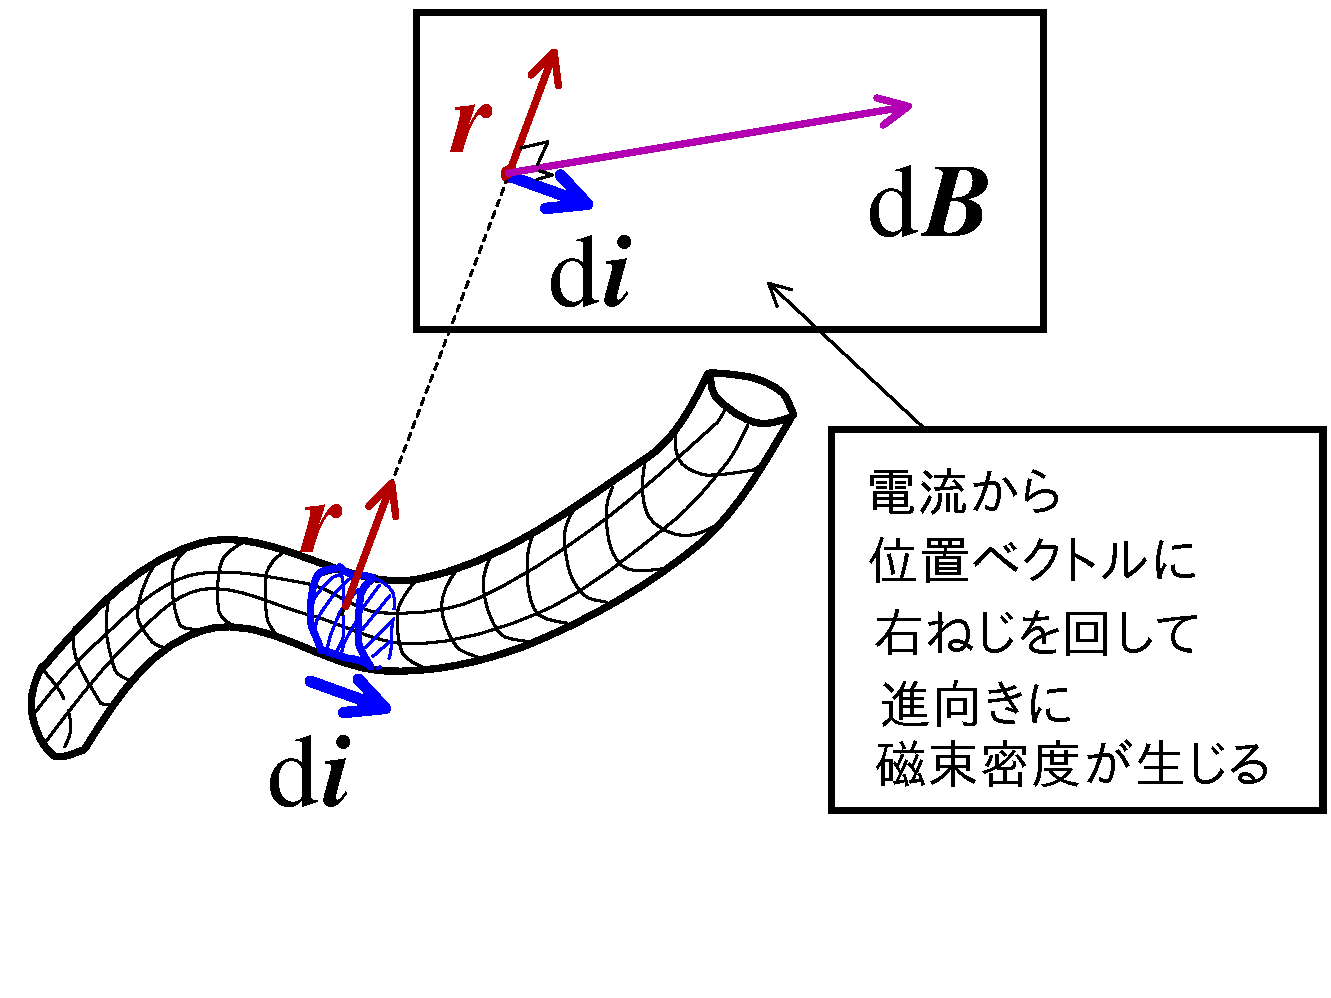
\includegraphics[keepaspectratio, width=7.2cm, height=5.79cm, clip]{biot_savart_1.pdf}
                    \caption{ビオ$=$サバールの法則}
                    \label{fig:biot_savart_1}
                \end{center}
            \end{figure}

    \subsection{点電荷の場合}
    最後に,電気量 $q$ をもつ点電荷に関する表示もしておこう.
    最初に示した式(\ref{Bior=savart'slow1})を思い起こそう.
        \begin{align*}
            \bB(\br)
            &=\frac{\mu_{0}|\bI|}{4\pi}
             \int_{\Gamma}\frac{\bt_{I}(\br')\times
                     (\br-\br')
                   }{|\br-\br'|^{3}}\df s' \\
            &=\frac{\mu_{0}}{4\pi}
             \int_{\Gamma}\frac{\bt_{I}(\br')\times
                     (\br-\br')
                    }{|\br-\br'|^{3}}|\bI|\df s'  \\
            \frac{\df \bB(\br)}{\df s'}
            &=\frac{\mu_{0}}{4\pi}
             \frac{\bt_{I}(\br')\times
                     (\br-\br')
                    }{|\br-\br'|^{3}}|\bI|  \\
            \df \bB(\br)
            &=\frac{\mu_{0}}{4\pi}
             \frac{\bt_{I}(\br')\times
                     (\br-\br')
                    }{|\br-\br'|^{3}}|\bI| \df s'  \\
            &=\frac{\mu_{0}}{4\pi}
             \frac{|\bI|\df s' \bt_{I}(\br')\times
                     (\br-\br')
                    }{|\br-\br'|^{3}}   \\
            &=\frac{\mu_{0}}{4\pi}|\bI|\df s' \bt_{I}(\br')\times
             \frac{(\br-\br')}{|\br-\br'|^{3}}
        \end{align*}

        ここで,\textbf{電流素片} という概念を導入しよう.
        上式の $|\bI|\df s' \bt_{I}(\br')$ に
        注目する.$\df s'$ は導線の微小な長さであるから,
        $|\bI|\df s' \bt_{I}(\br')$ という量は
        電流の微小な一部分であとみなせる.
        この $|\bI|\df s' \bt_{I}(\br')$ のことを電流素片と
        よぶことにしよう
            \footnote{
                教科書によっては,\textbf{電流要素} と表現されることもある.
            }.
        \begin{figure}[hbt]
            \begin{center}
                \includegraphicsdefault{dennryu_sohenn.pdf}
                \caption{電流素片 $|\bI|\df s \bt_{I}(\br)$}
                \label{fig:dennryu_sohenn}
            \end{center}
        \end{figure}


        電流素片 $|\bI| \df s'$ はその極限は,ひとつの点電荷の移動であると
        考えられる.点電荷の電気量を $q$,その速度を $\bv$ とすると,
        \begin{align*}
            |\bI| \df s' = q\bv.
        \end{align*}
        つまり,速度をもった点電荷が作る磁束密度 $\bB(\br)$ は
            \footnote{
                ここで,改めて,$\df \bB(\br)$ を $\bB(\br)$ に表示を置き換える.
                $\df \bB(\br)$ は電流の微小部分の作る磁束密度というイメージであったが,
                今考えている点電荷のつくる磁束密度であるので,それを $\bB(\br)$ と
                表現しても間違いではないだろう.いや,むしろこのように書き換えたほうが,
                式を自然な形にさせることができると思う.
            },
        \begin{align*}
            \bB(\br)
            &=\frac{\mu_{0}}{4\pi}q\bv \times
             \frac{\br-\br'}{|\br-\br'|^{3}}.
        \end{align*}
        \begin{myshadebox}{ビオ$=$サバールの法則(点電荷表示)}
            速度 $\bv$ で運動する,電気量 $q$ をもつ電荷は,次式で表される
            磁束密度 $\bB(\br)$ をその周囲に発生させる.
            \begin{align}
                \bB(\br)
                 &=\frac{\mu_{0}}{4\pi}q\bv \times
                  \frac{\br-\br'}{|\br-\br'|^{3}}.
            \end{align}
        \end{myshadebox}



%===================================================================================================
%  Chapter : 電磁気力(ローレンツ力)
%  説明    : 電磁気学的な力(電磁気力;ローレンツ力)の概念を導入する
%===================================================================================================
\chapter{電磁気力(ローレンツ力)}
%   %-----------------------------------------------------------------------------------------------
%   %  Input
%   %    File Name : PhysNote_EM_1st_LorentzForce.tex
%   %    説明      : クーロン力と磁束密度に関するローレンツ力を統合し,電磁気力を定める.
%   %-----------------------------------------------------------------------------------------------
        
%======================================================================
%  Section
%======================================================================
\section{ローレンツ力(電磁気力)}
    クーロン力 $\bF_{\mathrm{Coulomb}}$ と
    磁束密度に関するローレンツ力 $\bF_{\mathrm{Lorentz}}$ に
    よって,電気的な力と電荷が磁束密度より受ける力を記述する方法を得た.
        \begin{align*}
               & \bF_{\mathrm{Coulomb}} = q\bE. \\
                &\bF_{\mathrm{Lorentz}} = q\bv\times\bB.
        \end{align*}

    ところで,これまで「磁束密度に関するローレンツ力」という表現をしきりに使用
    してきた.わざわざ“磁束密度に関する”なんていう但し書きのような言い回しを
    してきたのには,理由がある.それは,単に \textbf{ローレンツ力} といった
    とき,それは
        \begin{align*}
            \bF &= \bF_{\mathrm{Coulomb}} + \bF_{\mathrm{Lorentz}} \\
                &= q(\bE + \bv\times\bB)
        \end{align*}
    のようなクーロン力と磁束密度に関するローレンツ力の和を指すからである
        \footnote{
            ちなみに,“電場に関するローレンツ力”なんてものは存在しない.ただ,
            磁束密度 $\bB$ や電荷 $q$ が0のときのような場合のローレンツ力は,
            クーロン力と等しくなり,電場に関するローレンツ力といっても間違い
            ではないとは思うが,一般的に通用する語彙ではない.
        }.
    \begin{myshadebox}{ローレンツ力}
        ある空間に電場 $\bE$ と磁束密度 $\bB$ が存在するとき,
        電気量 $q$ をもつ点電荷(以下,電荷 $q$ と書く)が
        速度 $\bv$ で運動しているならば,この電荷 $q$ には
        次式で示す \textbf{ローレンツ力} $\bF$ を受ける.
        \begin{align}
            \bF = q(\bE + \bv\times\bB)
        \end{align}
    \end{myshadebox}

\section{ローレンツ力と観測者}
        このローレンツ力は,不思議な力である.というのも,この力は
        観測者と電荷との相対的な速度 $\bv$ によっているからである.
        同じ電荷を観測していても,観測者によって電荷との相対速度
        が異なるのであれば,ローレンツ力の向きや大きさは,観測者ごとに
        異なったものとなる.なんとも不思議なことであるが,
        相対性理論を受け入れれば,何の不思議なことではなくなる.
        しかし,ここでは電磁気学を学ぶことが目標であるので,
        とりあえず,この不思議さは棚上げにしておき,話を
        先に進めることにしよう.


    \begin{memo}{電荷自身から発する磁束密度}
        電荷が磁束密度中を運動するときには,それにより磁束密度
        に関するローレンツ力を受け,速度の方向が変化してしまう.
        しかし,あとで述べるとおり,アンペールの法則によれば,
        磁束密度の発生源は電流である
            \footnote{
                アンペールの法則(※1)は
                次式で表現される.
                \begin{align*}
                    \drot\bB =  \mu_{0}\left(
                                    \bi + \frac{\rd \bE}{\rd t}
                                \right)
                \end{align*}
                言葉で表現すれば,大雑把に,
                \begin{align*}
                    \mbox{回転する磁束密度} = \mbox{電流} + \mbox{時間変動する電場}
                \end{align*}
                という感じになろう.詳しいことは,後に考える.

                (※1)正確には「アンペール$=$マクスウェルの法則」というべきだ.
            }.

        電荷が速度をもっていれば,
        それは電流と同一視できることになり,つまり,その物体自
        身がその周囲に磁束密度を生じさせていることになる.

        たしかに,はじめに考えたように,速度をもった電荷は,自身が
        発している磁束密度とは発生源が異なる磁束密度の影響をうけて,
        その方向が変化する.しかし一方で,電荷から発している磁束密度
        は,その周囲の磁束密度に影響を与えていることも事実である.

        そうであるとき,その影響はどの程度なのだろうか.それは,
        磁束密度に関するローレンツ力が $q\bv\times\bB$ と表される
        ことから,電荷の電気量 $q$ と速度 $\bv$ の大きさに依存している
        ことは明らかである.

        つまり,電荷を除いた状態での純粋な空間の磁束密度を $\bB_{\mathrm{pure}}$ と
        し,電荷から生じる磁束密度を $\bB_{\mathrm{q}}$ としたならば,電荷が
        存在する場合の正味の空間の磁束密度 $\bB$ は
            \begin{align*}
                \bB = \bB_{\mathrm{pure}} + \bB_{\mathrm{q}} \\
            \end{align*}
        である.だから,電荷が受ける磁束密度に対するローレンツ力は,
            \begin{align*}
                \bF &= q \bv \times \bB \\
                    &= q \bv \times (\bB_{\mathrm{pure}} + \bB_{\mathrm{q}}) \\
                    &= q \bv \times  \bB_{\mathrm{pure}} + q \bv \times \bB_{\mathrm{q}} \\
                \therefore\quad
                \bF &= q \bv \times  \bB_{\mathrm{pure}} + q \bv \times \bB_{\mathrm{q}}
            \end{align*}
        となり,$q \bv \times \bB_{\mathrm{q}}$ という分だけ,周囲の磁束密度を
        変化させ,それが自分の受ける磁束密度に対するローレンツ力に跳ね返ってくる.

        ここで気になるのは,$\bB_{\mathrm{q}}$ である.これは運動している電荷から
        発している磁束密度である.
        大きさはどのくらいで,どの方向に磁束密度は生じているのだろうか.
        これはビオ$=$サバールの法則から,位置 $\br$ に発生させる磁束密度 $\bB(\br)$ は
            \begin{align*}
                \bB_{\mathrm{q}}(\br) =
                \frac{\mu_{0}}{4\pi}q\bv \times
                \frac{\br-\br'}{|\br-\br'|^{3}}.
            \end{align*}
       と計算される.ここに,$\br'$ は磁束密度を観測する固定点である.
       とすれば,電荷が受ける磁束密度に対するローレンツ力は次のようになる.
            \begin{align*}
                \bF &= q \bv \times \bB_{\mathrm{pure}} + q \bv \times
                \left(
                    \frac{\mu_{0}}{4\pi}q\bv \times \frac{\br-\br'}{|\br-\br'|^{3}}
                \right) \\
                &= q \bv \times \bB_{\mathrm{pure}} + \frac{\mu_{0}}{4\pi}
                \left( q^{2} \bv \times \bv \times \frac{\br-\br'}{|\br-\br'|^{3}}
                \right).
            \end{align*}
        結果が見えてきた.ここで,ベクトル解析の公式,任意のベクトル $\bX$ に対して,
        $\bX \times \bX = \bzero$ を思い起こせば,
            \begin{align*}
                \bF &= q \bv \times \bB_{\mathrm{pure}} + \frac{\mu_{0}}{4\pi}
                \left(
                    q^{2} \bzero \times \frac{\br-\br'}{|\br-\br'|^{3}}.
                \right)\\
                &= q \bv \times \bB_{\mathrm{pure}} + \bzero \\
                \therefore\quad
                \bF &= q \bv \times \bB_{\mathrm{pure}}.
            \end{align*}
        この式の意味するところは,明白である.
        運動する電荷から発している磁束密度より受けるローレンツ力は,
        電荷自身に対して影響を及ぼさない,ということである.
        考えて見れば,簡単にイメージができることである.速度をもつ
        電荷がその周囲につくる磁束密度 $\bB_{\mathrm{q}}$ は,その速度に対して垂直な方向に
        生じる.なので,$\bB_{\mathrm{q}}$ は運動する電荷に対して,
        なんのエネルギーも与えないのだ
            \footnote{
                仕事の定義 $W = \bF \cdot \br$ を思い起こそう.物体に仕事を
                すると,それはエネルギーとして蓄えられるのだが,垂直成分は
                それに寄与しない.なぜなら,
                    \begin{equation*}
                        \bF \cdot \br = |\bF||\br| \cos \theta =  |\bF||\br| \cos(\pi/2) = 0.
                    \end{equation*}
            }.
    \end{memo}


%===================================================================================================
%  Chapter : マクスウェル方程式概観
%  説明    : マクスウェル方程式を帰納的に導く
%===================================================================================================
\chapter{マクスウェル方程式概観}
%   %-----------------------------------------------------------------------------------------------
%   %  Input
%   %    File Name : PhysNote_EM_1st_MaxEqImage.tex
%   %    説明      : マクスウェル方程式について,
%   %                その意味するところを言葉で大まかにイメージする
%   %-----------------------------------------------------------------------------------------------
        %   %==========================================================================
%   %  Section
%   %==========================================================================
    \section{4つの基本法則}\label{sec:4fundlaw}
    \begin{mycomment}
        ここでは,真空中の電磁気現象を想定する.言い換えれば,
        物質内のおける電場や磁束密度については想定していない.
        物質が存在する場合の理論は複雑になり,最初に学習する
        際には,理論の骨格を捉えにくいものである.理論の筋道を
        明確に捉えるために,真空中であるという制約を与える.
    \end{mycomment}

%       %======================================================================
%       %  SubSection
%       %======================================================================
        \subsection{はじめに}\label{subseq:4fundlaw_Hajimeni}
        電磁気的現象は4つの基本法則によって説明できる.ニュートン力学
        で言うところの,ニュートンの運動の3法則に対応する部分である.ついでに,
        それに対する方程式も記述しておこう.
            \begin{enumerate}
                \item 電場に対するガウス
                    \footnote{
                        Johann Carl Friedrich Gauss(Gau\ss)(1777--1855, ドイツ)
                        :ドイツの数学者,物理学者.整数や代数についての研究,曲
                        面論などに代表される幾何学の研究が有名である.近代数学の
                        大部分にその業績があり,19世紀最大の数学者とも言われる.
                        また,cgs単位系の「ガウス[G]」は磁気の単位として使われ
                        ている.そのほかにも,「ガウス記号(整数論)」,「ガウス
                        平面(複素関数論)」,「ガウス分布(誤差論)」など彼の名
                        がつけられた概念は多い.
                    }
                    の法則
                    \begin{align}
                        \ddiv \bE = \frac{1}{\varepsilon_{0}}\rho.
                    \end{align}
                \item 磁束密度に対するガウスの法則
                    \begin{align}
                        \ddiv \bB = 0.
                    \end{align}
                \item アンペール
                    =マクスウェル
                    \footnote{
                        James Clerk Maxwell(1831--1879, イギリス):古典電磁気学
                        の理論体系を築いた.この理論より電磁波の予言を行い,ヘル
                        ツ(Heinrich Rudolf Hertz, 1857--1894, ドイツ)らによって
                        実験的に実証された.

                        電磁気学的な自然現象は,4つの法則を基本法則とすることで,
                        説明のつく現象であると提唱する
                        (1865年;A dynamical theory of the electromagnetic field).
                        その後,マクスウェルは,1873年に,電磁気学を体系的に纏めた教科書を
                        出版し,電磁気学を確立させた
                        (1873年;A treatse on electricity and magnetism).
                        この教科書は,電磁気学におけるプリンキピアであると言われるようだ
                        (褒め言葉であると同時に,難解であるという意味も込められているらしい).

                        また,統計物理学の基本的な考え方である,気体分子運動論にかんする
                        研究も行なっている.「マクスウェル分布(マクスウェル--ボルツマン分布)」
                        としても,その名前を残している.これは今日の統計物理学の基礎をなすもの
                        である.

                        また,マクスウェルはキャベンディッシュ(\ref{sec:EM_ObjPreMsg}節の脚注を参照)
                        の仕事を世の中に紹介している.そして,当時新しく設けられた,
                        「キャベンディッシュ研究所」の実験物理学の教授(初代所長)として働いている.
                        なおこの研究所は,上に紹介したキャベンディッシュ(Henry Cavendish)の子孫
                        に当たる,デヴォンシャー第7大公爵が出資して作られた,
                        ケンブリッジ大学の実験物理学施設である.

                        片仮名表記される場合,「マックスウェル」とかかれることもある.

                        (参考1)太田 浩一,『マクスウェルの渦 アインシュタインの時計 現代物理学の源流』,
                        東京大学出版会

                        (参考2)William H.Cropper,『物理学天才外伝』, 講談社(ブルーバックス)
                    }
                    の法則
                    \begin{align}
                        \drot \bB = \mu_{0}\bi + \varepsilon_{0}\mu_{0}\frac{\rd \bE}{\rd t}.
                    \end{align}
                \item ファラデー
                    \footnote{
                        Michael Faraday(1791--1867, イギリス):電磁誘導の発見,
                        電気力線,磁力線の提唱(電磁気現象の近接作用の考え)など,
                        電磁気学に大きい貢献をする.また,化学者としての活躍も有名
                        であり,電気分解の法則の発見がその例である.コンデンサの容
                        量の単位「ファラド[F]」や,ファラデー定数などは,彼の名に
                        ちなんだものである.
                    }
                    の電磁誘導の法則
                    \begin{align}
                        \drot \bE = - \frac{\rd \bB}{\rd t}.
                    \end{align}
            \end{enumerate}

        以下では,これら4つの法則の内容をざっくりと見ていこう.その実験的根拠等の
        細かいことは,次章以降で考えることにする.ここでは,電磁気学は4つの基
        本法則から構成されているのだということを理解してもらいたい.
        各法則が意味する現象の詳細は,後で,それぞれ章を立てて説明する.

        もう一度注意しておこう.先のコメントの部分にも書いたが,以降で想定するのは,
        すべて,真空中で起こる電磁気現象である.物質を含む場合については,また別に
        議論することとにしたい.


%       %======================================================================
%       %  SubSection
%       %======================================================================
        \subsection{電場に対するガウスの法則}
        電場に対するガウスの法則は,電場の発生と消滅に関する法則である.内容は次
        の通りである.
            \\
            \begin{itembox}[l]{\textbf{電場に対するガウスの法則}}
                電場の\textbf{発生源}は\textbf{正に帯電した電荷}である.また,電
                場の\textbf{消滅源}は\textbf{負に帯電した電荷}である.そして,電
                場の発生と消滅は電荷においてのみ起こり,これ以外では起こらない.
            \end{itembox}
            \\

        この法則の意味するところは,電場の発生と消滅の原因は電荷にあることの主張
        である.正に帯電したから電荷から発生した電場は,負に帯電した電荷に吸収(
        消滅)するのである.そして,電場の発生,消滅は電荷以外では起こりえない.
               \begin{figure}[hbt]
                    \begin{tabular}{cc}
                        \begin{minipage}{0.5\hsize}
                            \begin{center}
                                \includegraphicsdouble{GaussLowImage_01.pdf}

                                (A) 正電荷より電場発生
                            \end{center}
                        \end{minipage}
                        \begin{minipage}{0.5\hsize}
                            \begin{center}
                                \includegraphicsdouble{GaussLowImage_02.pdf}

                                (B) 負電荷で電場消滅
                            \end{center}
                        \end{minipage}
                    \end{tabular}
                                \caption{電場に対するガウスの法則}
                                \label{fig:GaussLowImage}
                \end{figure}


%       %======================================================================
%       %  SubSection
%       %======================================================================
        \subsection{磁束密度に対するガウスの法則}
        磁束密度に対するガウスの法則は,磁束密度の発生と消滅に関する法則である.
        内容は次の通りである.
            \\
            \begin{itembox}[l]{\textbf{磁束密度に対するガウスの法則}}
                磁束密度の\textbf{発生源},\textbf{消滅源}は存在しない.
            \end{itembox}
            \\

        磁束密度がある点から生じて,他の点に吸収されるようなことは起こりえない
        ことを,この法則は主張する.つまり,電場の発生源とはる電荷に対応するよう
        な,言わば磁荷は存在しないことを意味する.
                \begin{figure}[hbt]
                    \begin{center}
                        \includegraphicsdefault{GaussLowBImage_01.pdf}
                        \caption{磁束密度に対するガウスの法則}
                        \label{fig:GaussLowBImage_01}
                    \end{center}
                \end{figure}

%       %======================================================================
%       %  SubSection
%       %======================================================================
        \subsection{ファラデーの電磁誘導の法則}
        ファラデーの電磁誘導の法則は,磁束密度の時間的な変化と電場の関係に関する
        法則である.内容は次の通りである.
           \\
           \begin{itembox}[l]{\textbf{ファラデーの電磁誘導の法則}}
               磁束密度が時間的に変化すると,その周囲には回転する電場が発生する.
           \end{itembox}
           \\

        磁束密度とは磁界のことだから,磁界の変化が回転する電場を発生させることに
        なる.具体的な例で考える.磁石は磁界を発生させていることは,中学生なら
        ば誰でもでも知っている.とすれば,磁界が変化する状況を作るには,磁石を手
        で持って振ればよい.ファラデーの電磁誘導の法則の法則は,この手で振ってい
        る磁石の周りに,電場が生じていると主張しているのである.
                \begin{figure}[hbt]
                    \begin{center}
                        \includegraphicsdefault{FaradayLowImage_01.pdf}
                        \caption{ファラデーの電磁誘導の法則}
                        \label{fig:FaradayLowImage_01}
                    \end{center}
                \end{figure}


%       %======================================================================
%       %  SubSection
%       %======================================================================
        \subsection{アンペール$=$マクスウェルの法則}
        アンペール$=$マクスウェルの法則は,電場の時間的な変化と磁束密度に関する法
        則である.内容は次の通りである.
            \\
            \begin{itembox}[l]{\textbf{アンペール$=$マクスウェルの法則}}
                電流の周りには,この電流を取り囲むように回転する磁束密度が生じる.ま
                たこれに加えて電場の状態が時間的に変化すると,その周囲には回転す
                る磁束密度が発生する.
            \end{itembox}
            \\

        電流が流れていると,その周りには磁界が発生しているということは,おそらく
        中学で習うはずだ.この法則では,それに加えて,時間的に変化する電場も,回
        転する磁束密度を作ることを主張している.
                \begin{figure}[hbt]
                    \begin{tabular}{cc}
                        \begin{minipage}{0.5\hsize}
                            \begin{center}
                                \includegraphicsdouble{AMLaw_Image00.pdf}

                                (A) 電流による磁場
                            \end{center}
                        \end{minipage}
                        \begin{minipage}{0.5\hsize}
                            \begin{center}
                                \includegraphicsdouble{AMLaw_Image01.pdf}

                                (B) 電場の時間変化による磁場
                            \end{center}
                        \end{minipage}
                    \end{tabular}
                        \caption{電流と時間変化する電場は,その周囲に回転する磁場を生じる}
                        \label{fig:AMLaw_Image00}
                \end{figure}

%   %==========================================================================
%   %  Section
%   %==========================================================================
    \section{マクスウェル方程式を見てみよう}
        \begin{mycomment}
            この節では,マクスウェル方程式を実際に見てみよう.
            だたし,その式をイメージとして捉え,意味すること
            を重視する.数式の本来の性質等は,各法則毎に詳しく
            調べることにし,ここでは数式の形に慣れることが目的
            である.徐々にマクスウェル方程式に馴染んで行こう.
        \end{mycomment}

%       %======================================================================
%       %  SubSection
%       %======================================================================
        \subsection{「マクスウェル方程式」とは}
        \begin{mycomment}
            まずは,「マクスウェル方程式」と言われる式について説明する.
            実は,マクスウェル方程式と言われてはいるが,マクスウェルがその
            方程式を発見したのではない.勘違いを起こしてしまいがちだが,
            マクスウェルが発見したという意味での,方程式は存在しないのである.
            ではどういうことかというと,言うなれば,
               “マクスウェルが提唱した,電磁気の公理的な4つの連立方程式”
            がマクスウェル方程式と呼ばれるものである.
        \end{mycomment}

%           %==================================================================
%           %  SubsubSection
%           %==================================================================
            \subsubsection{マクスウェルが電磁気学を確立する}
            電磁気的な自然現象には,冬場に発生する静電気や,より身近なものとして,
            磁石がある.携帯電話や無線LANも電磁気現象(電磁波)を利用した装置である.
            電磁気的な現象は,一見すると,その発生機構が複雑であるように感じてしまう.
            たしかに,マクスウェルにより指摘される以前では,電磁気現象は複雑であると
            感じることだったろう.しかし,今では,電磁気現象は,たった4つの法則を認め
            るだけで,説明ができることが分かっている.これを指摘した人物
            こそマクスウェルである.

            マクスウェルの提唱した4つの法則は,それ以前に先人
                \footnote{
                    例えば,アンペール,クーロンなどがいる.
                }
            により発見されていた自然現象をピックアップしたものであり,つまり,
            マクスウェル自身が4つの法則を発見したわけではない.マクスウェルの偉大なところ
            は,それまで煩雑としていた電磁気現象に関する実験結果(実験法則)を,体系化した
            ことにある.それまでには,色々な電磁気学の実験が行われて,その実験結果も
            多様にあったはずである.マクスウェルは,この煩雑な実験結果は,4つの自然現象
            を受け入れることで,すべてが上手く(数学的に)説明できることを示唆した.

%           %==================================================================
%           %  SubsubSection
%           %==================================================================
            \subsubsection{数式で表現してこそ,基本法則と言える}
            マクスウェルが基本法則として取り上げた4つの実験結果については,定性的には,
            上で紹介しと通りである(\ref{sec:4fundlaw}節参照).しかし,これらの法則は,
            数式により表現してこそ,意味を成す
                \footnote{
                    物理現象を説明するには,数式によりそれを表現すべきだ.
                    数式で表されて,初めて,詳細な推論や論理的思考が可能になるからだ.
                    数式を用いずに,言葉で表現しても論理的推論が不可能というわけではないが,
                    考えにくいし,論理もわかりにくくなる.数式で表現できれば,論理的
                    推論もしやすくなるし,論旨もわかりやすくなる.
                    不慣れな数式を扱うことが億劫かもしれなが,ここは少々なれるまで我慢
                    してもらいたい.物理学は数式を扱う学問なので,数式に慣れることは大事だ.
                    4つの法則で電磁気学現象を説明できるといったのは,各法則を方程式
                    で表したときに,電磁気現象が4つの方程式から数学的演算により,
                    論理的必然性をもった結果として導かれることをいう.
                }.
            そこで,次に,4つの基本法則を表す数式を紹介する.ただし,その数式に深入り
            することはせず,そのイメージを捉えることを第一の目的としたい.より詳しいことは,
            次章以降で考える
                \footnote{
                    実は,以下に説明する4つの方程式の理解こそが,初めて電磁気学を学ぶ際の
                    目標なのである.つまり,ここでは,その最終目標を先回りして紹介すること
                    になる.これは,学習の目標を明確にすることを考えてのことである.目標が
                    明確になれば,学習の際の不安(何をしているのかが分からないなど)も,少
                    しは解消されることと思う.
                }.

%           %==================================================================
%           %  SubsubSection
%           %==================================================================
            \subsubsection{マクスウェル方程式の2種類の表現}
            マクスウェル方程式は4つであるが,実は,その表現方法が2種類があり,
            微分を使って表現したものが \textbf{微分形},
            積分を使って表現したものが \textbf{積分形} と言われる.ここでは,
            この2種類の表現方法を紹介する.微分形と積分形の違いは,視点の違いである.
            現実に起こっている現象を肌で感じる場合には,積分形の方程式を用いる.
            そのため,工学の分野では,積分形を使うことのほうが多いと思う.これに対し,
            微分形で記述されたものは,現象を局所的に見た場合に使われる.微分形は
            理論的考察を行う場合に使うことが多い.もちろん,積分形で表されようが,
            微分形で表されようが,その式は全く等価である(当たり前のはずだが,念のために).


%       %======================================================================
%       %  SubSection
%       %======================================================================
        \subsection{約束:独立変数の記述の省略}
                マクスウェル方程式は,位置 $\br$ と時間 $t$ の4つの独立変数を
                含む関数の間に成り立つ式であるが,この独立変数をいちいち明記
                していたら,式が煩雑になり見難くなっていしまう.そこで,
                以下のように,独立変数を省略して記述する.
                すなわち,
                電場 $\bE$,磁束密度 $\bB$,電流密度 $\bi$,電荷密度 $\rho$ であり,
                その意味は次式の通り.
                    \begin{align*}
                        \bE  &= \bE(\br,\,t) \\
                        \bB  &= \bB(\br,\,t) \\
                        \bi  &= \bi(\br,\,t) \\
                        \rho &= \rho(\br,\,t)
                    \end{align*}
                また,$\varepsilon_{0}$,$\mu_{0}$ は,それぞれ,真空中の誘電率,透磁率と言われる,
                スカラー量で,単なる定数である(位置と時間の関数ではない).

                ついでに,他の記号も説明する.
                任意の閉曲面を $S$ で表現する.また,$S$ で囲まれた内部の領域全体を $\Omega_{S}$ と
                書く.閉曲面の微小部分は $\df S$ であり,
                $\df S$ の単位法線ベクトルは $\bn:=\bn(\br,\,t)$ で表現する.
                また,$l$ は任意の閉経路(ループしている経路,輪状の経路のこと)である.そして,$S_{l}$ というのは,
                閉経路 $l$ を縁とする開曲面を表す.そして,閉経路 $l$ の単位接線ベクトルを $\bt:=\bt(\br,\,t)$ と
                表現する.

                くどいかもしれないが,演算に関する記述方法の説明もしておこう.
                $\sint_{S} X\df S$ は,関数 $X$ を,$S$ に対して面積分を行うことを意味する.また,
                $\vint_{\Omega_{S}} X \df V$ は,関数 $X$ を,$S$ の内側の全領域 $\Omega_{S}$ に
                対して体積分を行うことを意味する.

%       %======================================================================
%       %  SubSection
%       %======================================================================
        \subsection{マクスウェル方程式(微分形)}
        \begin{mycomment}
            上では,現実に起こっている法則のイメージを説明したが,
            ここではもう一歩先に進んで数式を眺めてみよう.この節では,
            微分形のマクスウェル方程式を確認する.積分形も,後で確認する.
            何度も言うが,
            数式そのものを理解することが目的ではなく,数式のイメージを
            持つことが目的である.数式の詳細は後で述べる.ここではとにかく,
            求めるべきマクスウェル方程式がどのようなものかを,感覚的に
            把握してもらいたい.
        \end{mycomment}
%           %==================================================================
%           %  SubsubSection
%           %==================================================================
            \subsubsection{電場に対するガウスの法則の式:微分形}
            \begin{mysmallsec}{数式}
                電場に対するガウスの法則の,微分形の式は次式の通り.
                \begin{align}
                    \ddiv \bE = \frac{1}{\varepsilon_{0}}\rho.
                \end{align}
            \end{mysmallsec}

            \begin{mysmallsec}{法則のイメージ}
                電場の発生あるいは消滅は,電荷の存在する場所で生じる.また,言い換えれば,
                ある場所において,電場が発生あるいは消滅していることと,その場所に電荷が
                存在することは,同じ意味をなす.

                ベクトル $\bE$ は電場で,その前に書かれている $\ddiv$ は,
                divergence(発散) を意味する.なので,左辺 $\ddiv \bE$ は電場の発散を表す.
                右辺の$\rho$ は電荷密度
                    \footnote{
                        1/$\varepsilon_{0}$ がかかっているが,単なる比例定数である.
                        これは単位系としてSI単位を採用していることによって現れた定数
                        であり,式の表す物理的イメージにはあまり関係がないと思って良い.
                    }
                であり,電荷密度の存在が表されている.
                電場の発散と電荷密度が等号で結ぶことによって意味されることは,
                「電荷密度が存在すれば,その周囲には電場の発散が生じる」ということである.
                更にその逆もいうことができて,「電場の発散の原因は電荷密度である」ということも
                できる.
                電場の発生あるいは消滅は,電荷の存在しない場所では,絶対に発生しない.
            \end{mysmallsec}

                \begin{figure}[hbt]
                    \begin{center}
                        \includegraphicsdefault{GaussLowEImage_03.pdf}
                        \caption{電場は電荷より生じる}
                        \label{fig:GaussLowEImage_03}
                    \end{center}
                \end{figure}

%           %==================================================================
%           %  SubsubSection
%           %==================================================================
            \subsubsection{磁束密度に対するガウスの法則の式:微分形}
            \begin{mysmallsec}{数式}
                磁束密度に対するガウスの法則の,微分形の式は次式の通り.
                \begin{align}
                    \ddiv \bB = 0.
                \end{align}
            \end{mysmallsec}

            \begin{mysmallsec}{法則のイメージ}
                この式は,磁束密度はどこからも湧き出しがないことを表現している.
                見方を変えれば,ある部分で湧き出す磁束密度の量と,その部分で消滅する
                磁束密度の量が等しいから,正味として湧き出しがないとみなされる.

                つまり,磁束密度の発生場所を特定することはできないということである.
                こういう言い方すると,“磁束密度は存在して,その発生原因は電流にあることを,
                先に説明している.つまり,発生している場所を示すことができるではないか”と
                いう疑問を持たれてしまうかもしれない
                    \footnote{
                        少なくとも,私はそう思った.
                    }.
                しかし,これは言葉の意味の捉え方(あるいは記述の仕方)の問題であり,
                磁束密度の存在場所が特定できないことを言っているのではない.この法則は
                ,あくまでも,発生源を特定することができないということであり,発生して
                いる場所を示せないということではない.現に,磁石の周囲には磁束密度が存在
                していることは,すでに知っていることである.たしかに,磁石から磁束密度が
                湧き出していると考えても,間違いではないが,この法則の言っている「湧き出し」とは
                意味がことなる.先にも書いたとおり,ここで言う「湧き出し」とは,磁束密度の
                生じる量と消滅する量の,“正味の湧き出し”ということである.この正味の湧き出しが
                0であるというとは,この世界のどの場所を見ても磁束密度の正味の湧き出しがないという
                ことを意味しているのである.この「正味の」という部分に,注意すべきだ.
            \end{mysmallsec}

                \begin{figure}[hbt]
                    \begin{center}
                        \includegraphicsdefault{GaussLowBImage_02.pdf}
                        \caption{磁束密度の湧き出しはない}
                        \label{fig:GaussLowBImage_02}
                    \end{center}
                \end{figure}


%           %==================================================================
%           %  SubsubSection
%           %==================================================================
            \subsubsection{アンペール$=$マクスウェルの法則の式:微分形}
            \begin{mysmallsec}{数式}
                アンペール$=$マクスウェルの法則の式の,微分形の式は次式の通り.
                \begin{align}
                    \drot \bB = \mu_{0}\bi + \varepsilon_{0}\mu_{0}\frac{\rd \bE}{\rd t}.
                \end{align}
            \end{mysmallsec}

            \begin{mysmallsec}{法則のイメージ}
                右辺に項が2つあるが,これらはそれぞれ,意味することが異なる.
                右辺の第一項は,電流が磁場を作るということを主張するものである.
                これは,アンペールの法則とよばれる
                    \footnote{
                        アンペールの法則とは,上式の第二項が常に0である場合のことである.
                        すなわち,次式がアンペールの法則を表す式である.
                            \begin{align}
                                \drot \bB = \mu_{0}\bi.
                            \end{align}
                        アンペールの法則の意味するところは,式を見れば明らかである.
                        口うるさく意味を説明すれば,
                        「回転している磁束密度が存在するということは,その内側の領域に
                        電流が生じていることを意味する」ということだ.
                    }.
                そして,第二項が意味するのが,
                \textbf{変位電流} という概念である.詳細は後述するが,ここでは,
                おおよそのイメージとして,電場の時間変化がその周囲に磁束密度を
                生じさせる,と解釈して欲しい
                    \footnote{
                        式をそのまま言葉にしただけである.その真意の程は後の記述を
                        参照.
                    }.

                なぜ,「変位電流」を導入する必要があるのかというと,単なるアンペールの法則が
                電荷保存則に矛盾してしまうからである.つまり,アンペールの法則と電荷保存則の
                どちらかが,間違っている(不完全である)可能性があるということである
                    \footnote{
                        あるいは,どちらとも間違いなのかもしれない.しかしこの可能性は,
                        あとに記述する,マクスウェルの修正によってなくなる.
                    }.
                マクスウェルによる回答は,アンペールの法則が不完全である,ということだった.
                そして,マクスウェルはアンペールの法則を完全な形にすべく,「変位電流」という
                新しい概念を考案し,アンペールの法則にそれを組み込むことで,電荷保存則との
                矛盾を解消したのである.

                あとに分かることだが,この変位電流は,ファラデーが発見する電磁誘導の法則
                に対をなす現象である,と見ることもできる.この変位電流と電磁誘導とにより,
                電磁波という現象が起こるのである.電磁波についても,後ほど考えることにしたい
                    \footnote{
                        マクスウェル方程式の偉大さの一つは,電磁波の存在を予言したことである.
                    }.

                もう一度改めて,この法則の内容を確認しておこう.電流はその周囲に磁束密度を
                発生させる.さらに,それに加えて,電場の時間変化が起きた際にも,その電場の
                変化にともなって,その周囲に,磁束密度が生じるのである.
            \end{mysmallsec}

                \begin{figure}[hbt]
                    \begin{tabular}{cc}
                        \begin{minipage}{0.5\hsize}
                            \begin{center}
                                \includegraphicsdouble{dennryu_to_jisokumitudo.pdf}

                                (A) 電流による磁場
                            \end{center}
                        \end{minipage}
                        \begin{minipage}{0.5\hsize}
                            \begin{center}
                                \includegraphicsdouble{hennnidenryu_to_jisokumitudo.pdf}

                                (B) 変位電流による磁場
                            \end{center}
                        \end{minipage}
                    \end{tabular}
                        \caption{電流,変位電流と磁束密度の関係}
                        \label{fig:I_i_B}
                \end{figure}


%           %==================================================================
%           %  SubsubSection
%           %==================================================================
            \subsubsection{ファラデーの電磁誘導の法則の式:微分形}
            \begin{mysmallsec}{数式}
                ファラデーの電磁誘導の法則の式の,微分形の式は次式の通り.
                \begin{align}
                    \drot \bE = - \frac{\rd \bB}{\rd t}.
                \end{align}
            \end{mysmallsec}

            \begin{mysmallsec}{法則のイメージ}
                左辺は回転する電場を表している.右辺は負の符号がついて入るが,
                磁束密度の時間変化が記述されている.渦を巻くように電場が生じている
                ならば,その周囲に磁束密度の時間変化が起こっているということを示している.
                また,言い方を変えれば,磁束密度が時間変化するとき,その周囲に渦を巻くようにして
                電場が生じるということでもある.磁束密度の時間変化とは,現実的に言えば,例えば
                磁石を左右に振った場合のことである.このとき左右にふった磁石の周りには,その磁石を
                取り囲むように,渦電場が生じるのである.
            \end{mysmallsec}

%       %======================================================================
%       %  SubSection
%       %======================================================================
        \subsection{マクスウェル方程式(積分形)}
%           %==================================================================
%           %  SubsubSection
%           %==================================================================
            \subsubsection{電場に対するガウスの法則の式:積分形}
            \begin{mysmallsec}{数式}
                電場に対するガウスの法則の,積分形の式は次式の通り.
                \begin{align}
                    \sint_{S} \bE \cdot \bn \df S = \frac{1}{\varepsilon_{0}} \vint_{\Omega_{S}} \rho \df V.
                \end{align}
            \end{mysmallsec}

            \begin{mysmallsec}{法則のイメージ}
                この式の言っていることは,微分形のそれと同じだが,次のような
                イメージを連想させる.すなわち,ある領域 $S$ から電場が湧き出ている
                ならば,その内部領域 $\Omega_{S}$ に電荷が存在しする.そして,このとき湧き出す電場の量
                は,$\Omega_{S}$ 内に存在するすべての電荷の電気量の総和
                を $\varepsilon_{0}$(真空中の誘電率;詳細は後述する)で割った値に等しい.

                要するに,ある領域から電場が生じているのであれば,その領域には
                必ず電荷が存在するということである.
            \end{mysmallsec}

%           %==================================================================
%           %  SubsubSection
%           %==================================================================
            \subsubsection{磁束密度に対するガウスの法則の式:積分形}
            \begin{mysmallsec}{数式}
                磁束密度に対するガウスの法則の,積分形の式は次式の通り.
                \begin{align}
                    \sint_{S} \bB \cdot \bn \df S = 0.
                \end{align}
            \end{mysmallsec}

            \begin{mysmallsec}{法則のイメージ}
                この式の意味は,微分形のそれと全く同様である.

                この表現のほうが,イメージしやすいかもしれない.任意の領域 $S$ を
                設定しても,そこから生じる正味の磁束密度の量は0であることを,
                表現している.つまり,磁束密度の湧き出し場所が,$S$ 内部ではない
                ということである.といっても,湧き出しはどこか別の場所($S$ の外側)に
                あるということではない.$S$ は任意に設定できる閉曲面であるから,
                $S$ をどんな風にとっても,磁束密度の発生源は $S$ の内部ではないという
                ことになる.つまり,この世界の至る場所で,磁束密度の湧き出し量が
                正味0であるということだ.

                電場に対するガウスの法則は,電場の発生原因を電荷に押し付けいているのに対し,
                磁束密度に対するこの法則は,いわば「磁荷」が存在しないということを意味する.
                磁束密度に対して,なぜ「磁荷」がないのだろうかといった疑問も強いことと思う.
                実際,物理学者の中でもその存在を信じ,探している人もいるらしい.しかし,
                このノートでは,この現象を実験事実として認め,深入りは避けることとしたい
                    \footnote{
                        実は,特殊相対性理論を学習すると,磁束密度は,光速不変の原理と
                        特殊相対性理論から導かれるローレンツ力と,クーロンの法則から導
                        出することができてしまう.電場の発生原因は電荷にあり,電荷はク
                        ーロンの法則に従った動きをする.他方,物体が光の速さで運動する
                        さいには,ローレンツ変換に従う.とどの詰まりは,電荷が光速で運
                        動する際に,静止している観測者には,その周囲に磁束密度が分布し
                        ているようにみえてしまうのである.これは,ローレンツ力に関連す
                        る.先に,ローレンツ力は,観測者と電荷との相対速度 $\bv$ が関
                        係していることを見た.この相対速度こそが,磁束密度の存在を支え
                        ているのである.磁束密度は,観測者と電荷の相対的な関係により,
                        生じるものであると,考えることもできるのである.このことを定量
                        的に考えることは,相対論を学習した後で行うことにしよう.
                    }.
            \end{mysmallsec}

%           %==================================================================
%           %  SubsubSection
%           %==================================================================
            \subsubsection{アンペール$=$マクスウェルの法則の式:積分形}
            \begin{mysmallsec}{数式}
                アンペール$=$マクスウェルの法則の式の,積分形の式は次式の通り.
                \begin{align}
                    \oint_{l} \bB \cdot \bt \df l
                    = \sint_{S_{l}} \left( \bi + \varepsilon_{0}\frac{\rd \bE}{\rd t} \right) \cdot \bn \df S_{l}.
                \end{align}
            \end{mysmallsec}

            \begin{mysmallsec}{法則のイメージ}
                この式の意味するところは,ある閉曲線 $l$ の内側を観察したとき,
                磁束密度が生じているのであれば,$l$ を境界とする曲面 $S_{l}$ を
                電流が貫いているか,もしくは電場の時間変化が生じているということ
                である.電場の時間変化と電流は,その周囲に磁束密度を発生させるのである.

                この積分形の式の左辺により,生じる磁束密度の総量が計算される.右辺は,
                閉曲面 $S_{l}$ に生じている全電流と電場の時間変化の総量が計算される.
                つまり,全電流と電場の時間変化の総量を計算することで,生じる磁束密度の総量
                がわかるのである.
            \end{mysmallsec}

%           %==================================================================
%           %  SubsubSection
%           %==================================================================
            \subsubsection{ファラデーの電磁誘導の法則の式:積分形}
            \begin{mysmallsec}{数式}
                ファラデーの電磁誘導の法則の式の,積分形の式は次式の通り.
                \begin{align}
                    \oint_{l} \bE \cdot \bt \df l
                    = -\frac{\rd}{\rd t} \sint_{S_{l}} \bB \cdot \bn \df S_{l}.
                \end{align}
            \end{mysmallsec}

            \begin{mysmallsec}{法則のイメージ}
                磁束密度の時間変化は,その周囲に回転する電場を発生させることを,
                この式は意味している.

                微分形の式は,生じているか否かを判定するものであるが,
                この積分形の式は,生じる電場の総量が計算できる.
                閉ループ $l$ に導線を重ねあわせて導線の輪を作り,
                その導線の輪の内側において磁束密度を変化させると,
                導線に起電力が生じる.この起電力の大きさは,どの程度磁束密度を
                変化させたかによって決まる.その計算式が,積分形の電磁誘導の法則の
                式である.
            \end{mysmallsec}


%===================================================================================================
%  Chapter : 電場に対するガウスの法則
%  説明    : 電場に対するガウスの法則をクーロンの法則から導く
%===================================================================================================
\chapter{電場に対するガウスの法則}
%   %-----------------------------------------------------------------------------------------------
%   %  Input
%   %    File Name : PhysNote_EM_1st_GaussLowEF.tex
%   %-----------------------------------------------------------------------------------------------
        %   %==========================================================================
%   %  Section
%   %==========================================================================
    \section{電場の定義}
    \subsection{クーロンの法則(復習)}
        \begin{mycomment}
            クーロンの法則についての詳細は,\ref{sec:CoulomnbForce}節を参照.
            以下は,そこからの抜粋である.
        \end{mycomment}

            ここに,電荷が2つあるとしよう.この2つの電荷は区別する
            ことができて,$q_{1}$,$q_{2}$ という電気量を持っている
            とする.電荷 $q_{1}$ と $q_{2}$ との距離を $r$ としたと
            き,この2つの電荷が受ける力は,以下のような規則がある.
            \begin{itemize}
                \item 2つの電荷の電気量が互いに異なる符号をもってい
                      るならば,両電荷は互いに引き合う向きに力を受
                      ける
                \item 2つの電荷の電気量が同じ符号を持っているならば,
                      両電荷は互いに反発しあう向きに力を受ける.
                \item 2つの電荷の受ける力の大きさは等しく,
                      向きは互いに逆向きである
                \item 2つの電荷が受ける力の大きさは,
                      2つの電荷の電気量の積($q_{1}q_{2}$)に比例する.
                \item 2つの電荷が受ける力の大きさは,
                      2つの電荷間の距離の2乗($r^{2}$)に反比例する.
            \end{itemize}

        図\ref{fig:coulombs_low}をもう一度載せておこう.
        \begin{figure}[hbt]
            \begin{tabular}{cc}
                \begin{minipage}{0.5\hsize}
                    \begin{center}
                        \includegraphicsdouble{coulombs_low1.pdf}
                    \end{center}
                \end{minipage}
                \begin{minipage}{0.5\hsize}
                    \begin{center}
                        \includegraphicsdouble{coulombs_low2.pdf}
                    \end{center}
                \end{minipage}
            \end{tabular}
        \end{figure}


            次の数式によって,クーロンの法則は表現される.

            電荷 $q_{1}$ に対して働く力は,以下.
               \begin{align}\label{eq:coulomb_force_f1_2nd}
                   \bF_{21} =
                       \frac{1}{4\pi\varepsilon_{0}} \frac{q_{1}q_{2}}{r^{2}}
                           \frac{\br_{1} - \br_{2}}{|\br_{1} - \br_{2}|}.
               \end{align}

            電荷 $q_{2}$ に対して働く力は,以下.
               \begin{align}
                   \bF_{2} = -\bF_{1} =
                       \frac{1}{4\pi\varepsilon_{0}} \frac{q_{2}q_{1}}{r^{2}}
                           \frac{\br_{2} - \br_{1}}{|\br_{2} - \br_{1}|}.
               \end{align}


        \begin{figure}[hbt]
            \begin{center}
                \includegraphicsdefault{Coulombs_Force.pdf}
            \end{center}
        \end{figure}


%   %==========================================================================
%   %  Subsection
%   %==========================================================================
    \subsection{電場に対するガウスの法則の導出}
        \begin{mycomment}
            ガウスの法則は,言っていることは単純だが,数式を用いて説明されると,
            慣れないうちは何のことだかサッパリわからないことだろう.なので,
            どの教科書でも取られている手段だが,まずは単純な場合から考えて,
            徐々に一般化していこう.まず,点電荷1個より生じる電場の満たす
            法則を考える.次に,電荷の個数を増やし,$N$ 個の点電荷にする.
            最後に,最も一般的な連続分布する電荷より生じる電場の満たす法則を
            考える.また,電場のみが存在し,磁束密度は存在しないとして,
            議論が煩雑になるのを避けることとする
                \footnote{
                    このような仮定をすることに,注意しておこう.
                    時間的に変動する電磁場についてはこのように考えることはできない,
                    ということである.理由は,判例を示すのが手っ取り早い.
                    中学生のときに, \textbf{電磁誘導の法則} に
                    よって,『磁石を動かしたときに,電流が生じる』という現象を
                    観測した(はずである).磁石を動かすことは
                    磁束密度を変化させることを意味し,
                    電流が発生するということは導体内に
                    電場が生じたということになる.
                    つまり,磁束密度が時間的に変化すると,電場が発生するのである.
                    このことを考えると,動電磁場の場合は電場と磁束密度を
                    分けて考えることはできないのである.電磁誘導の法則についての詳しいことは,動電磁場の
                    部分で確認する.
                }.
        \end{mycomment}
%       %======================================================================
%       %  Subsection
%       %======================================================================
        \subsubsection{クーロンの法則から見えてくること}
            クーロンの法則によって定義された電場 が満たしている法則を考える.
            2つの点電荷における,クーロンの法則を書き下そう.
                \begin{align}
                    F  =  \frac{1}{4\pi \varepsilon_{0} } \frac{q_{1}q_{2}}{r^{2}}.
                \end{align}
            ここに,$q_{1}$,$q_{2}$ は電荷の電気量であり,$r$ は
            2つの点電荷間の距離である.ここでは,大きさのみを考える.
            さてこの時,電気量 $q_{1}$ をもつ電荷が作る電場を考えると,
                \begin{align}
                    E_{1}  =  \frac{1}{4\pi \varepsilon_{0}} \frac{q_{1}}{r^{2}}.
                \end{align}
            いま,興味があるのは,この電場 $E_{1}$ が満たす法則である.
            次のように書き変えてみよう.
                \begin{equation*}
                    E_{1}  =  \frac{1}{4\pi \varepsilon_{0}} \frac{q_{1}}{r^{2}}
                            =  \frac{1}{4\pi r^{2}} \frac{q_{1}}{\varepsilon_{0}}
                \end{equation*}
            さて,この式の $4\pi r^{2}$ の部分に注目する.これは,球の
            表面積の公式と同じである.そこで,これを球の表面積
            としてみなし,記号 $S$ で置き換えてみよう.
                \begin{equation*}
                    E_{1}  =  \frac{1}{S} \frac{q_{1}}{\varepsilon_{0}}
                \end{equation*}
            両辺に $S$ をかける.
                \begin{equation*}
                    E_{1}S  =   \frac{q_{1}}{\varepsilon_{0}}
                \end{equation*}

            ところで,球の面積 $S$ は,積分記号を用いて面積分
            の形で表現すると,
                \begin{equation*}
                    S = \int_{S} \df S
                \end{equation*}
            である.$S$ は球の表面全体を表すと同時に,その表面積でもある.球の
            表面である $S$ を微小分割して,かき集めたものが,
            球の面積である.
            これを用いると,電場の式は
                \begin{equation*}
                    E_{1}\int_{S} \df S  =   \frac{q_{1}}{\varepsilon_{0}}
                \end{equation*}
            となる.
            さて,球の面の法線ベクトルと点電荷が作る電場の向きは,
            球のどの部分でも一致する.しがって,上式の電場 $E_{1}$ は,
            球の面積積分の中に入れてさしつつ変えない.つまり,
                \begin{equation*}
                    \int_{S} E_{1}\df S  =   \frac{q_{1}}{\varepsilon_{0}}
                \end{equation*}
            とできる.

            実は,この式が求めている式なのである.
            すなわち,上式が電場が従う法則である.
            言葉で表せば,次のようになる:点電荷 $q_{1}$ が
            球面 $S$ の内部に存在するとき,
            その周囲につく電場 $E_{1}$ を球面 $S$ で面積分すると,
            $q_{1}/\varepsilon_{0}$ という値になる.

            この法則を,\textbf{ガウスの法則} という.
            しかし,今得られたガウスの法則を,さらに一般化することが
            できる.次の項目で,このガウスの法則を一般化しよう.

%       %======================================================================
%       %  Subsection
%       %======================================================================
        \subsubsection{1つの点電荷のみが存在する場合}
            点電荷が1個しかない状況を想定し(図\ref{fig:Gauss_1tendenka}),
            この1個の点電荷から生じる電場が満たす法則について考える.
                        \begin{figure}[hbt]
                            \begin{center}
                                \includegraphicsdefault{Gauss_1tendenka.pdf}
                                \caption{閉曲面$S$の中に1つの電荷を含む場合}
                                \label{fig:Gauss_1tendenka}
                            \end{center}
                        \end{figure}

            1つの点電荷が作る電場を書き下すと,
                \begin{align}
                    \bE(\br)
                    &=\frac{1}{4\pi\varepsilon_{0}}\int_{\Omega_{S}}
                    \frac{q\delta(\br-\br^{*})}
                         {|\br-\br^{*}|^{2}}
                    \frac{\br-\br^{*}}
                         {|\br-\br^{*}|}\df V^{*}
                \end{align}
            である.(電場の定義式(\ref{denba})
            で $\rho(\br^{*})
            =q\delta(\br-\br^{*})$ と置けばよい.)
            ここで, $1/4\pi\varepsilon_{0}$ は定数であるので積分記号の前に出した.
            点電荷の位置を $\br^{*}$ として,$\br^{*}=0$ と
            原点を定める.すると,
                \begin{align*}
                    \bE(\br)
                    &=\frac{1}{4\pi\varepsilon_{0}}
                    \frac{\displaystyle\int_{\Omega_{S}}
                    q\delta(\br)\df V}{|\br|^{2}}
                    \frac{\br}
                         {|\br|}  \\  \\
                    &=\frac{1}{4\pi\varepsilon_{0}} \int_{\Omega_{S}}
                    q\delta(\br)\df V
                    \frac{1}{|\br|^{2}}
                    \frac{\br}
                         {|\br|}
                \end{align*}
            と書ける.この式の両辺を,$\Omega_{S}$ の表面である閉曲面 $S$ で面積分する.
                \begin{align*}
                    &\int_{S}\bE(\br)\cdot\textit{\textbf{n}}(\br)\df S \\
                    &=\frac{1}{4\pi\varepsilon_{0}}
                    \int_{S}\left( \int_{\Omega_{S}} q\delta(\br)\df V \right)
                    \frac{1}{|\br|^{2}}
                    \frac{\br}
                         {|\br|}\cdot\textit{\textbf{n}}(\br)\df S.
                \end{align*}
            この場合,右辺の体積積分と面積分 は関係がないので
                \footnote{
                        体積積分を先に計算する必要があり,この体積積分の部分は定数になる.
                },体積積分を
            面積分の外に出すことができる.
            この式の体積積分の部分は,系の電気量の総和を計算するものであり,定数であると考えられるのである.
                \begin{align*}
                    &\int_{S}\bE(\br)\cdot\textit{\textbf{n}}(\br)\df S \\
                    &=
                    \frac{1}{4\pi\varepsilon_{0}}
                    \left(\int_{\Omega _{S}}q\delta(\br)\df V \right)
                    \left(\int_{S} \frac{1}{|\br|^{2}}
                    \frac{\br}{|\br|} \cdot \textit{\textbf{n}}(\br)\df S \right) \\
                    &=
                    \frac{1}{4\pi\varepsilon_{0}}
                    \left(\int_{\Omega _{S}}q\delta(\br)\df V \right)
                    \left(\int_{S} \frac{\br}{|\br|^{3}}
                    \cdot \textit{\textbf{n}}(\br)\df S \right).
                \end{align*}
            ここで,公式
                    \begin{align}
                        \int_{S}\frac{\br}{|\br|^{3}}
                        \cdot\textit{\textbf{n}}(\br)\df S&=4\pi\qquad S\supset 0(=\br^{*})
                    \end{align}
            を用いると $4\pi$ が消えて,
                \begin{align}
                    \int_{S}\bE(\br)\cdot\textit{\textbf{n}}(\br)\df S
                    &=\frac{1}{\varepsilon_{0}}\int_{\Omega_{S}}q\delta(\br)\df V
                \end{align}
            を得る.

            点電荷が閉曲面 $S$ の内側である場合,
            すなわち,点電荷が領域 $\Omega_{S}$ 内に存在する場合,$\delta$ 関数の性質によって,
                \begin{align}
                    \int_{S}\bE(\br)\cdot\textit{\textbf{n}}(\br)\df S
                    &=\frac{q}{\varepsilon_{0}}
                \end{align}
            である.もし点電荷が領域 $\Omega_{S}$ 内に存在しない場合,
                \begin{align}
                    \int_{S}\bE(\br)\cdot\textit{\textbf{n}}(\br)\df S
                    &=0
                \end{align}
            である.

            ここで特に不安になるのは,点電荷が閉曲面 $\Omega_{S}$ に含まれていない場合に,果たして本当に
            ガウスの法則を満たしているかということである.というのも,閉曲面 $\Omega_{S}$ を任意にとることができる
            ので,もしかしたら,この閉鏡面のとり方によってはガウスの法則を満たさない場合が生じてしまうかもしれない
            からである.しかし,この不安は不要である.上で導出したガウスの法則は公式
                    \begin{align}
                        \int_{S}\frac{\br}{|\br|^{3}}
                        \cdot\textit{\textbf{n}}(\br)\df S&=4\pi\qquad S\supset 0
                        (=\br^{*})
                    \end{align}
            により,どのような閉曲面をとっても満たすということが保証されているからである.といっても,
            直感的にわかるはずもないので,以下で,このことを説明してみよう.まず,任意に閉曲面 $\Omega_{S}$ をとる.
            このとり方で,複雑な形にとる場合には図\ref{fig:gauss_s_low2}が当てはまるだろう.
            図\ref{fig:gauss_s_low2}以外のより複雑に,閉曲面 $\Omega_{S}$ をとったとしても,この図の
            とり方を発展させたものとして考えれば理解できるだろう.図では任意の閉鏡面を水色で
            描いた.
                \begin{figure}[hbt]
                    \begin{tabular}{cc}
                        \begin{minipage}{0.5\hsize}
                            \begin{center}
                                \includegraphicsdouble{GaussLow2.pdf}
                                \caption{ガウスの法則 (1)}
                                \label{fig:GaussLow2}
                            \end{center}
                        \end{minipage}
                        \begin{minipage}{0.5\hsize}
                            \begin{center}
                                \includegraphicsdouble{gauss_s_low2.pdf}
                                \caption{ガウスの法則 (2)}
                                \label{fig:gauss_s_low2}
                            \end{center}
                        \end{minipage}
                    \end{tabular}
                \end{figure}


%       %======================================================================
%       %  Subsection
%       %======================================================================
        \subsubsection{$N$ 個の点電荷のみが存在する場合}
            もう少し一般化して,電荷の数を複数にしよう.
            電荷の個数を2個とか,3個とかの具体的な数にせず,$N$ 個として,少し
            一般性をもたせて考える.
                \begin{figure}[hbt]
                    \begin{center}
                        \includegraphicsdefault{Gauss_huku_tendenka.pdf}
                        \caption{閉曲面 $S$ の中に複数の電荷を含む場合}
                        \label{fig:Gauss_huku_tendenka}
                    \end{center}
                \end{figure}
            複数の点電荷が存在する場合の電場は式(\ref{denba_huku})から,
            \begin{align}
                \bE(\br)&=\sum_{i=1}^{N}\frac{1}{4\pi\varepsilon_{0}}
                \frac{q_{i}}{|\br-\br_{i}|^{2}}
                \frac{\br-\br_{i}}
                     {|\br-\br_{i}|}
            \end{align}
            と書ける.すなわち,一つひとつの点電荷が作る電場を足し合わせればよい.
            この式の両辺を任意の閉曲面 $S$ で面積分すると,
            \begin{align*}
                &\int_{S}\bE(\br)\cdot\textit{\textbf{n}}(\br)\df S \\
                &=\frac{1}{4\pi\varepsilon_{0}}\int_{S} \sum_{i=1}^{N}
                \frac{q_{i}}
                    {|\br-\br_{i}|^{2}}
                \frac{\br-\br_{i}}
                     {|\br-\br_{i}|}\cdot\textit{\textbf{n}}(\br_{i})\df S
            \end{align*}
            各点電荷について,
            \begin{align}
            q_{i}=\int_{\Omega_{S}}q_{i}\delta(\br-\br_{i})\df V
            \end{align}
            であるから,
            \begin{align*}
                &\int_{S}\bE(\br)\cdot\textit{\textbf{n}}(\br)\df S \\
                &=\frac{1}{4\pi\varepsilon_{0}}\int_{S} \sum_{i=1}^{N}
                \frac{\displaystyle\int_{\Omega_{S}}q_{i}\delta(\br-\br_{i})\df V}
                {|\br-\br_{i}|^{2}}
                \frac{\br-\br_{i}}
                     {|\br-\br_{i}|}\cdot\textit{\textbf{n}}
                    (\br_{i})\df S \\
            \end{align*}

            右辺の $\int_{\Omega_{S}}q_{i}\delta(\br-\br_{i})\df V$ に
            注目する.$N$ 個の点電荷のうち,領域 $\Omega_{S}$ の外側に存在する点電荷は何らこの積分に
            関与しない.なぜなら,そのような点電荷を領域 $\Omega_{S}$ で体積積分したところで,
            その値は $\delta$ 関数の性質によって,0 になるからである.従って,
            領域 $\Omega_{S}$ 内の点電荷だけについて考えればよいことになる.
            逆に考えれば,領域 $\Omega_{S}$ の外側の点電荷については,全く存在しないものとして扱う
            ということである.

            では,式変形に戻る.この場合も,右辺の体積積分と面積分 は関係がないので
                \footnote{
                        体積積分を先に計算する必要があり,この体積積分の部分は定数になる.
                },
            体積積分を
            面積分の外に出すことができる.
            この式の体積積分の部分は,系の電気量の総和を計算するものであり,定数であると考えられる.
            \begin{align*}
                &\int_{S}\bE(\br)\cdot\textit{\textbf{n}}(\br)\df S \\
                &=\frac{1}{4\pi\varepsilon_{0}}
                \sum_{i=1}^{N}
                    \biggl\{
                        \left(
                            \int_{\Omega_{S}}q_{i}\delta(\br-\br_{i})\df V
                        \right)
                                                [A]
                     \biggr\}
            \end{align*}
                        ここで,面積積分に相当する $[A]$ の部分は式が長くなるたに一時的に導入した文字で,以下のとおりである.
                                \begin{align}
                            [A] = \int_{S} \frac{\br-\br_{i}}{|\br-\br_{i}|^{3}}
                                          \cdot \textit{\textbf{n}}(\br_{i})\df S
                                \end{align}
            この面積積分 $[A]$ については,前にも確認したように,公式
            \begin{align}
                [A] = \int_{S}
                \frac{\br-\br_{i}}
                {|\br-\br_{i}|^{3}}\cdot\textit{\textbf{n}}(\br_{i})\df S
                =4\pi
            \end{align}
            が成り立つので,
            \begin{align}
                \int_{S}\bE(\br)\cdot\textit{\textbf{n}}(\br)\df S
                &=\sum_{i=1}^{N}\int_{\Omega_{S}}\frac{1}{\varepsilon_{0}}
                q_{i}\delta(\br-\br_{i})\df V \notag \\
                &=\frac{1}{\varepsilon_{0}}\int_{\Omega_{S}}\sum_{i=1}^{N}q_{i}
                \delta(\br-\br_{i})\df V
            \end{align}
            を得る.さらにわかりやすくすると,$\Omega_{S}$ 内に存在する電荷 $Q_{\mbox{内}}$ と書けば,
            \begin{align}
            Q_{\mbox{内}}=\int_{\Omega_{S}}\sum_{i=1}^{N}q_{i}\delta(\br-\br_{i})\df V
            \end{align}
            となることから,
            \begin{align}\label{denba_N0-2}
                \int_{S}\bE(\br)\cdot\textit{\textbf{n}}(\br)\df S
                &=\frac{Q_{\mbox{内}}}{\varepsilon_{0}}
            \end{align}
            と表現することも可能である.

%       %======================================================================
%       %  Subsection
%       %======================================================================
        \subsubsection{電荷が連続的に分布する場合}
            \begin{figure}[hbt]
                \begin{center}
                    \includegraphicsdefault{Gauss_renzoku_tendenka.pdf}
                    \caption{閉曲面$S$の中に点電荷が連続的に分布している場合}
                    \label{fig:Gauss_renzoku_tendenka}
                \end{center}
            \end{figure}
            電荷が連続的に分布しているときは,$N$ 個の電荷が存在するときの $Q_{\mbox{内}}$ を
            各点電荷の電気量の和ではなく,電荷密度 $\rho(\br)$ の
            積分に変更すればよい.
            すなわち,
            \begin{align}
                Q_{\mbox{内}}&=\int_{\Omega_{S}}\rho(\br)\df V
            \end{align}
            とすればよい.これを式(\ref{denba_N0-2})代入することにより,以下の式を得る.
                    \begin{myshadebox}{静電場のガウスの法則(積分形)}
                        \begin{align}
                            \int_{S} \bE(\br)\cdot\textit{\textbf{n}}(\br)\df S
                            =\frac{1}{\varepsilon_{0} }\int_{\Omega_{S}} \rho (\br) \df V
                        \end{align}
                    \end{myshadebox}

            この式が求めるべき \textbf{静電場に対するガウスの法則} である.

            電場に対するガウスの法則は,クーロンの法則の上に成り立つものである.
            なぜなら,電場はクーロンの法則から定義される量であるからである.
            従ってガウスの法則は,今の立場からは,法則とはいえない.
            しかし,電磁場を考えるときには,ガウスの法則
            を基礎とした方が都合がよい(場の近接的な作用など).
            だから,「法則」とよばれるのである.
            (ガウスの法則は,力学と電磁気学の関連を考える上でも重要な法則の1つとなる.)


%   %==========================================================================
%   %  Subsection
%   %==========================================================================
    \subsection{法則の意味(定性的なイメージ)}
%       %======================================================================
%       %  Subsection
%       %======================================================================
        \subsubsection{法則のイメージ}
            何度も述べてきた法則のイメージだが,ここで再度,確認したい.

            結論の式を言葉で表現すれば,
            領域 $\Omega_{S}$ の表面 $S$ から流出する電場 $\bE(\br)$ は
            領域 $\Omega_{S}$ 内部の電気量の総和の $1/\varepsilon_{0}$ に等しいと解釈できる.

            ガウスの法則の具体的なイメージは,微分形の方程式を導くことによって,よりよく得られる.
            しかし,先に述べた指針(積分形の導出を優先すること)により,ここでは微分形の方程式を
            考えることは控える.とはいえ,イメージできなければこのような法則などは
            頭に入ってこない.そこで,ここではそのイメージを先取りして書いておく.
            具体的な式については,微分形の導出のところで確認する.

            微分形のガウスの法則は,『正の電気量をもつ電荷から電場が生じ,負の電荷にその電場が吸収される』と
            いったことを表す.正の電荷から電場が湧き出して,負の電荷で電場が消えていくといったほうが
            イメージしやすい.
            とにかくここでは,「電場というものは,正の電荷から発生し,負の電荷で吸収される」
            と理解しておく.そして,電場の流出量(もしくは吸収量)について語ってくれるのが
            積分形のガウスの法則である.

            積分形のガウスの法則は,前にも言ったように,系全体を眺めた時の式である.例として,
            正の電気量をもつ電荷1つを考える.この電荷が内側に入り込むように閉曲面 $S$ をとる.
            この電荷から,電場が湧き出ているイメージをする.どの程度の電場が流出しているのだろうか.
            積分形のガウスの法則の示すところによると,この閉曲面 $S$ から流出する
            電場は,どんな閉曲面をとろうが電荷がその閉曲面の内側に入っていれば,一定の値を示すのである.
            その値は閉曲面に包まれた電荷の電気量の $1/\varepsilon_{0}$ 倍である.
            もちろん,その閉曲面内に電荷が入っていなければ,電場の流出量は 0 であることもいえる.

            とりあえずここでは,「電場の流出量が 積分形のガウスの法則によって計算できる」ということを
            頭に入れておく.

            注意しておく.静電場とは,固定された電荷による電場の流出量が一定で時間変化しないということである.
            絶えず電場を発生させているのであるので,電場が止まっているわけではない.電場は
            流れ続けているのである.ただ,全ての位置において,電場の流れの方向が時間変化しない
            ということから,静電場というのである.具体的にいえば,位置 $\br_{1}$ を
            指定すると,いつでも時間に関係なく,$\bE(\br_{1})$
            の電場が流れているということである.

%       %======================================================================
%       %  Subsection
%       %======================================================================
        \subsubsection{近接作用するクーロン力}
            さて,これでようやく遠隔作用のクーロン力を近接作用として
            受け入れることができる.もう一度,状況を確認すると,2つの
            点電荷が距離 $r$ を隔てて
            固定されているとしたのであった.このとき,一方の電荷 $q_{1}$ から生じた電場が,
            徐々にもう一方の電荷 $q_{2}$ の
            位置に伝わって,クーロン力を及ぼす.強調しておきたいことは,
            電荷 $q_{1}$ が直接的にもう一方電荷 $q_{2}$ にクーロン力を及ぼすのではなく,$q_{1}$ から
            生じる電場を介して,電荷 $q_{2}$ にクーロン力が伝わるということである.
            クーロン力の伝わる速さは光速である.それは後に示すように,電場は光速で伝わることからいえることである.
            さて,この時点で「クーロン力が伝わる」という表現が“何かおかしい”と感じるだろう.
            実際,伝わるのは電場であって,クーロン力そのものが伝わるわけではない.
            電場が伝わるのである.電場を主役にするために
            実験法則であるクーロンの法則が,電場に対するガウスの法則に書き換えられたのは当然
            であると考えてようだろう.しかし,電場の存在の裏には,クーロンの法則が
            隠れていることを忘れてはいけない.あくまでも,電場は試験電荷が受けるクーロン力
            として定義されるものである.

            ちょっと混乱したかもしれない.念のため,補足しておこう.
            電場の存在を確認するには
            試験電荷が必要だが,電場がどのように伝わるかを
            考えるときには試験電荷を持ってくる必要はない.
            電磁気学の基本方程式を考えるという視点から考えれば,
            電場に対するガウスの法則を考えればよく,クーロン力は
            補助的な式として捉えるべきだ.


%   %==========================================================================
%   %  Section
%   %==========================================================================
    \section{電位}
%       %======================================================================
%       %  Subsection
%       %======================================================================
        \subsection{クーロン力より生じるポテンシャル$\cdot$エネルギー}
            おそらく,電位の定義をいきなり述べても,理解が難しいことだろう.
            なので,ここで導入として,簡略化した話を記述しておく.
            詳細は,この節のあとに記述する.まずは,イメージをもってもらいたい.

            一次元で考える.クーロンの力の大きさは,クーロンの法則から,
                \begin{equation*}
                    F=
                    \frac{1}{4 \pi \varepsilon}
                    \frac{q_{1}q_{2}}{{r}^{2}}
                \end{equation*}
            である
                \footnote{
                    方向をつけて書くと
                        \begin{equation*}
                            F=
                            \frac{1}{4 \pi \varepsilon}
                            \frac{q_{1}q_{2}}{{r}^{2}}
                            \frac{\br}{r}
                        \end{equation*}
                    である.一次元であっても,正方向と負方向があるので,
                    方向も記述すべきだ.ここでは,大きさのみを考えるので,
                    方向を示す単位ベクトル $\br/r$ は考慮しない.
                }.
            ここに,$q_{1}$,$q_{2}$ は点電荷のもつ電気量であり,
            $r$ は2つの点電荷間の距離である.

            このクーロン力より生じる,ポテンシャル$\cdot$エネルギーを
            計算しよう.2つの点電荷のうち,一つを固定して,この固定された
            電荷がつくるポテンシャルを考える.もう一方の点電荷は自由に動ける
            ようにしておく.添字に意味もたせたいので,以下のように付け替えておこう.
                \begin{align*}
                    q_{1} := q_{0}\,, \quad q_{2} := q_{x}
                \end{align*}
            こうすると,クーロンの法則は,
                \begin{equation*}
                    \frac{1}{4 \pi \varepsilon}
                    \frac{q_{0}q_{x}}{{r}^{2}}
                \end{equation*}
            と書かれる.$q_{x}$ を動かすことで,$q_{0}$ が
            つくるポテンシャルを計算する.

            $q_{0}$ の位置を $r_{0}$ とし,
            $q_{x}$ の位置を $r_{x}$ と書いたとき,
            距離は $r = | r_{x} - r_{0} |$ とかけるが,
            固定する電荷の位置を原点にすれば($r_{0}=0$ とすれば)
                \begin{equation*}
                    r = r_{x}
                \end{equation*}
            とできる.クーロンの法則は,次のようになる.
                \begin{equation*}
                    \frac{1}{4 \pi \varepsilon}
                    \frac{q_{0}q_{x}}{{r_{x}}^{2}}.
                \end{equation*}

            基準点を無限遠($\infty$)にとり,$q_{0}$ が $q_{x}$ に及ぼす
            クーロン力の仕事を計算することで,ポテンシャルが計算できる
                \footnote{
                    これがポテンシャルのエネルギーの定義なのだから.
                }.
            つまり,
            $r_{x}$ で無限遠から任意の位置 $x$ まで
            積分(広義積分)するということである.
                \begin{figure}[hbt]
                    \begin{center}
                        \includegraphicsdefault{denni_Image.pdf}
                        \caption{電位と仕事}
                        \label{fig:denni_Image}
                    \end{center}
                \end{figure}

            計算は
            以下のように実行できる.
                \begin{align*}
                  &\int_{\infty}^{r_{0}}
                        \frac{1}{4 \pi \varepsilon}
                        \frac{q_{0}q_{x}}{{r_{x}}^{2}}
                    \df r_{x} \\
                  &=
                    \frac{q_{0}q_{x}}{4 \pi \varepsilon}
                    \int_{\infty}^{r_{0}}
                        \frac{1}{{r_{x}}^{2}}
                    \df r_{x} \\
                  &=
                    \frac{q_{0}q_{x}}{4 \pi \varepsilon}
                    \biggl[
                        -\frac{1}{r}
                    \biggr]_{\infty}^{r_{0}} \\
                  &=
                    \frac{q_{0}q_{x}}{4 \pi \varepsilon}
                    \biggl[
                        -\frac{1}{r_{0}} - \left( -\frac{1}{\infty} \right)
                    \biggr].
                \end{align*}
            ここで,$1/\infty \rightarrow 0$ として
                \footnote{
                    次式を計算していることと同じ.
                    \begin{equation*}
                        \lim_{x \rightarrow 0} \frac{1}{x} = 0.
                    \end{equation*}
                },
                \begin{align*}
                   &\frac{q_{0}q_{x}}{4 \pi \varepsilon}
                    \biggl[
                        -\frac{1}{r_{0}} - \left( -\frac{1}{\infty} \right)
                    \biggr] \\
                  &=
                    \frac{q_{0}q_{x}}{4 \pi \varepsilon}
                    \left(
                         - \frac{1}{r_{0}}
                    \right) \\
                  &=
                    -\frac{q_{0}q_{x}}{4 \pi \varepsilon} \frac{1}{r_{0}}.
                \end{align*}
            よって,
                \begin{align*}
                    \int_{\infty}^{r_{0}}
                        \frac{1}{4 \pi \varepsilon}
                        \frac{q_{0}q_{x}}{{r_{x}}^{2}}
                    \df r_{x}
                  =
                    -\frac{q_{0}q_{x}}{4 \pi \varepsilon} \frac{1}{r_{0}}.
                \end{align*}
            計算は以上で終了.

            最後に,$r_{0}$ に一般性をもたせておこう.固定する位置を,
            改めて,任意の位置 $r$ とし,
                \begin{equation*}
                    r=r_{0}
                \end{equation*}
            と置き換える.すると,
            任意の位置 $r$ に存在する点電荷のポテンシャルを表現できるようになる.
            また,今までは $q_{x}$ に及ぼす仕事を考えてきたが,これを単位電荷にすると,
            つまり,
                \begin{equation*}
                    q_{x} = 1[\mathrm{C}]
                \end{equation*}
            とすれば,単位電荷あたりの仕事になる.

            この電気的なポテンシャルを表す記号として,$\phi$ を用いると,
            以下のようになる.
                \begin{align}
                    \phi
                    :=
                    \int_{\infty}^{r_{0}}
                        \frac{1}{4 \pi \varepsilon}
                        \frac{q_{0}q_{x}}{{r_{x}}^{2}}
                    \df r_{x}
                    =
                    -\frac{q_{0}}{4 \pi \varepsilon} \frac{1}{r}.
                \end{align}
            これが,求めたかったポテンシャル$\cdot$エネルギーである.

            この式の,右辺に注目しよう.今まで積分をしてきたわけであるが,
            今度は逆に微分してみよう.すると,次のようになる.
                \begin{align*}
                    \frac{\rd \phi}{\rd \br}
                  &= \frac{\rd}{\rd \br}
                        \left(
                            -\frac{q_{0}}{4 \pi \varepsilon} \frac{1}{r}
                        \right) \\
                  &= \frac{q_{0}}{4 \pi \varepsilon} \frac{1}{r^{2}}.
                \end{align*}
            この右辺は固定されている点電荷より生じる電場 $E_{0}$ に他ならない
                \footnote{
                    \begin{equation*}
                        E_{0} = \frac{q_{0}}{4 \pi \varepsilon} \frac{1}{r^{2}}.
                    \end{equation*}
                }.
            すなわち,
                \begin{align*}
                    \frac{\rd \phi}{\rd \br} = E_{0}
                \end{align*}
            となる.これは,次のように書いても同じことである.
                \begin{align*}
                    \phi = \int_{\infty}^{r} E_{0} \df r.
                \end{align*}

            まとめておこう.まず,クーロン力によるポテンシャル$\cdot$エネルギーを
            計算した
                \footnote{
                    実は,電場からも計算できるのだが,ポテンシャルは力から
                    導いた方が定義に沿っているので,今回はこの導出方法を
                    記述した.
                }.
                \begin{align}
                    \phi := -\frac{q_{0}}{4 \pi \varepsilon} \frac{1}{r}.
                \end{align}
            そして,このポテンシャルから,微分を使って,電場との関係を
            導いた.
                \begin{align*}
                    \frac{\rd \phi}{\rd \br} = E_{0}
                    , \quad \mathrm{or}, \quad
                    \phi = \int_{\infty}^{r} E_{0} \df r.
                \end{align*}


%       %======================================================================
%       %  Subsection
%       %======================================================================
        \subsection{電位の定義}
            力学でポテンシャル・エネルギーは重力によるものであった.
            それと同じように,電場によるポテンシャル・エネルギーを考える.
            以下では,ポテンシャル・エネルギーのことを,
            単に「ポテンシャル」と省略して書くことにする.このノートでは,電場のポテンシャルを
            表す記号として $\phi$ を用いることにする.
            ポテンシャルは,位置 $\br$ の関数であるから
            ,$\phi(\br)$ と
            書くこともある.

            電気的なポテンシャルを \textbf{電位} と定義する.以下の通り.
                \begin{myshadebox}{電位の定義}
                    電位 $\phi(\br)$ を,下式で定義する.
                    \begin{align}
                        \phi(\br) := -\int_{C} \bE(\br) \cdot \df\br
                    \end{align}
                \end{myshadebox}


%       %======================================================================
%       %  Subsection
%       %======================================================================
        \subsection{電位の定義の意味}
            電気量 $q'$ [C]をもつ電荷が,電場が 0 である
            位置 $\br_{0}$ に固定されているとする.
            この電荷を,電場の存在する位置 $\br$ まで変位させることを考える.
            まず,この電荷が電場 $\bE(\br)$ から
            受ける力 $\bF(\br)$ を考えると,それはクーロン力であり,
            \begin{align}
                \bF(\br)=q'\bE(\br)
            \end{align}
            と書ける.
            よって,この力 $\bF(\br)$ に抗して,
            外力 $-\bF(\br)$ で電荷を変位させることになる.
            このとき,外力のする仕事 $W$ は
            \begin{align}
                W&=\int_{C} -\bF(\br) \cdot \df\br \notag \\
                &=\int_{C} -q'\bE(\br) \cdot \df\br
            \end{align}
            である.従って,単位電荷(つまり $q=1[C]$)当りに,
            \begin{align}
                W_{q'=1[c]}=\int_{C} -\bE(\br) \cdot \df\br
            \end{align}
            だけの仕事をすることになる.この式は電位の式に他ならない.


%       %======================================================================
%       %  Subsection
%       %======================================================================
        \subsection{電場と電位の関係}
            電場と電位の関係を導出する.この関係は静電場の基本法則の導出につながるものである.
            \begin{align}
            \phi(\br) := -\int_{C} \bE(\br) \cdot \df\br
            \end{align}
            ここで,$\bE=(E_{x},E_{y},E_{z})$,$\df\br=(\df x,\df y,\df z)$ のように
            成分表示すると,上の定義式は
                \begin{align}
                    \phi(\br)
                    =-\int_{C} E_{x}\df x+E_{y}\df y+E_{z}\df z
                \end{align}
            と書ける.従って,
                \begin{align}
                    E_{x}=-\frac{\rd \phi(\br)}{\rd x} \,\,,
                    \,\,\,E_{y}=-\frac{\rd \phi(\br)}{\rd y} \,\,,
                    \,\,\,E_{z}=-\frac{\rd \phi(\br)}{\rd z}
                \end{align}
            とかける.ベクトルとしてまとめれば,
                \begin{align}
                    \bE
                    =\left(-\frac{\rd \phi(\br)}{\rd x}\,\,,
                    \,\,\,-\frac{\rd \phi(\br)}{\rd y}\,\,,
                    \,\,\,-\frac{\rd \phi(\br)}{\rd z}
                            \right)
                \end{align}
            この式を以下のように変形する.
                \begin{align}
                    \bE
                    =-\left(\frac{\rd}{\rd x},
                      \frac{\rd}{\rd y} ,
                      \frac{\rd}{\rd z}
                      \right) \phi(\br)
                \end{align}
            ここで,力学のときにも確認したように,
                \begin{align}
                    \dgrad
                    =\left(\frac{\rd}{\rd x},
                      \frac{\rd}{\rd y} ,
                      \frac{\rd}{\rd z}
                      \right)
                \end{align}
            という勾配を導出する演算子を考えれば,
                \begin{align}
                    \bE = -\dgrad\phi(\br)
                \end{align}
            の関係を得ることができる.
                    \begin{myshadebox}{静電場と静電ポテンシャルの関係}
                        電場とは電位の勾配でもある.
                        \begin{align}
                            \bE = -\dgrad\phi(\br).
                        \end{align}
                    \end{myshadebox}

            この式は,静電場の場合だけに成り立つ関係である.

            \begin{memo}{ポテンシャルを基礎に,電場を定義する場合}
                今日では,ポテンシャルの概念より電場を定義することが多い.
                これは解析力学などによって,ポテンシャルの重要性が
                浮かび上がったことからも想像できることだろう.従って,
                次のように考えることになる.

                電気的なポテンシャル,すなわち電位 $\phi$ が存在するとき,
                電場は以下のように定義される.
                \begin{align}
                    \bE  := -\dgrad \phi =-\frac{\rd \phi}{\rd \br}
                \end{align}
                電位の存在するかどうかを調べるには,空間に試験電荷を置いて見ればよい.電位が存在していれば,
                点電荷は電位勾配によって運動し始めるはずである.そしてこのとき,
                電位勾配とは逆向きの電場が生じていると考えるのである.
            \end{memo}

%       %======================================================================
%       %  Subsection
%       %======================================================================
        \subsection{等電位面}
            電位の等しい値の点をつなぐと,それは1つの曲面をなす.1つの点において,電位を
            2つ以上もつことはないからである.そのような曲面を \textbf{等電位面} という.
            式で表現すると,電位の値を $\phi_{0}$ として,
                \begin{align}
                    \phi(\br)=\phi_{0}
                \end{align}
            である.等電位面のイメージは下図のようである.
                \begin{figure}[hbt]
                    \begin{tabular}{cc}
                        \begin{minipage}{0.5\hsize}
                                \begin{center}
                                    \includegraphicsdouble{toudenimen_monopole.pdf}
                                    \label{fig:toudenimen0}

                                    (a) 平面的

                                \end{center}
                        \end{minipage}
                        \begin{minipage}{0.5\hsize}
                                \begin{center}
                                    \includegraphicsdouble{Potentiol_monopole.pdf}
                                    \label{fig:toudenimen1}

                                    (b) 立体的
                                \end{center}
                        \end{minipage}
                    \end{tabular}
                    \caption{単一電荷の作る等電位面}
                \end{figure}

                \begin{figure}[hbt]
                    \begin{tabular}{cc}
                        \begin{minipage}{0.5\hsize}
                                \begin{center}
                                    \includegraphicsdouble{toudenimen.pdf}
                                    \label{fig:toudenimen2}

                                    (a) 平面的
                                \end{center}
                        \end{minipage}
                        \begin{minipage}{0.5\hsize}
                                \begin{center}
                                    \includegraphicsdouble{Potentiol_dipole.pdf}
                                    \label{fig:toudenimen3}

                                    (b) 立体的
                                \end{center}
                        \end{minipage}
                    \end{tabular}
                    \caption{異種の2電荷がつくる等電位面}
                \end{figure}


%       %======================================================================
%       %  Subsection
%       %======================================================================
        \subsection{等電位面と電場の向き}\label{subsec:toudeni_denba}
            等電位面内にベクトル $\br$ をとる.このベクトルが位置する等電位面の
            電位は $\phi(\br)$ である.
            同じ等電位面において,ベクトル $\br$ より少しだけずれた $\br+\df\br$ を
            とる.もちろん,ベクトル $\br$ と $\br+\df\br$ は同じ等電位面に
            存在しているので,
                \begin{align}
                    \phi(\br)=\phi(\br+\df\br)=\phi_{0}
                \end{align}
            の関係がある.$\phi(\br)=\phi(\br+\df\br)$ の両辺を
            位置 $\br$ で テイラー展開 して,
                \begin{align}
                    \phi(\br)=\phi(\br)
                    +\frac{\rd \phi(\br)}{\rd \br}\df x
                    +\frac{\rd \phi(\br)}{\rd \br}\df y
                    +\frac{\rd \phi(\br)}{\rd \br}\df z
                \end{align}
            である.ここで,右辺については2次以上の項は無視した.従って,
                \begin{align}
                    \frac{\rd \phi(\br)}{\rd \br}\df x
                    +\frac{\rd \phi(\br)}{\rd \br}\df y
                    +\frac{\rd \phi(\br)}{\rd \br}\df z=0
                \end{align}
            となる.ここで,
                \begin{align}
                    \frac{\rd}{\rd \br}=\dgrad \quad, \quad \df\br=\left( \df x,\df y,\df z \right)
                \end{align}
            であることに注意すると,
                \begin{align}
                    \dgrad\phi(\br)\cdot \df\br=0
                \end{align}
            となる.最後に,電場と電位の関係式から,
                \begin{align}
                    \bE(\br)\cdot \df\br=0
                \end{align}
            を得る.この式の $\df\br$ は初めに考えた等電位面内の
            ベクトルである.このベクトルと電場の内積が 0 であるという結果かが
            得られたのである.すなわち,『電場と等電位面は直交する』ということを
            表現している.
                \begin{figure}[hbt]
                    \begin{center}
                        \includegraphicsdefault{DengaToToudenniMen001.pdf}
                        \caption{等電位面と電場}
                        \label{fig:DengaToToudenniMen001}
                    \end{center}
                \end{figure}

%       %======================================================================
%       %  Subsection
%       %======================================================================
        \subsection{ポアソン方程式}\label{subsec:pisson_eq}
            電荷分布が与えられれば,電位や電場が計算できるはずである.
            その計算に用いる方程式が,\textbf{ポアソン方程式} である
                \footnote{
                    Sim\`{e}on Denis Poisson(1781--1840, フランス):数学者.
                    ポアソン方程式,ポアソン分布,ポアソン括弧など,物理学に
                    寄与する数学を築き上げた人.
                }.
            ガウスの法則:
                \begin{equation*}
                    \ddiv \bE = \frac{\rho(\br)}{\varepsilon_{0}}
                \end{equation*}
            の $\bE$ に,電場と電位の関係:
                \begin{equation*}
                    \bE = - \dgrad \phi(\br)
                \end{equation*}
            を代入して,$\bE$ を消去すると,
                \begin{equation*}
                    \ddiv \left( \dgrad \phi(\br) \right) = - \frac{\rho(\br)}{\varepsilon_{0}}.
                \end{equation*}
            ここで,以下を定義する.
                \begin{align}
                    \nabla := \left(\frac{\rd}{\rd x} ,\, \frac{\rd}{\rd y} ,\, \frac{\rd}{\rd z}\right).
                \end{align}
            この記号 $\nabla$ は \textbf{ナブラ} とよばれる微分演算子である.$\nabla$ を用いると,上式は,次
            のようにも表現できる.
                \begin{equation*}
                    {\nabla}^{2} \phi(\br) = - \frac{\rho(\br)}{\varepsilon_{0}}.
                \end{equation*}
            さらに,$\Lap$ を以下で定義する.
                \begin{align}
                    \Lap := {\nabla}^{2}.
                \end{align}
            この微分演算子 $\Lap$ を \textbf{ラプラシアン} という.$\Lap$ を用いると,
                \begin{align}\label{eq:pisson_eq}
                    \Lap \phi(\br) = - \frac{\rho(\br)}{\varepsilon_{0}}.
                \end{align}
            を得る.この式(\ref{eq:pisson_eq})を \textbf{ポアソン方程式} という
                \footnote{
                    「ポアソンの方程式」と表現されることも多い.
                }.

%       %======================================================================
%       %  Subsection
%       %======================================================================
        \subsection{ラプラス方程式}\label{subsec:laplace_eq}
            ポアソン方程式の定数項を0とおいた式を,\textbf{ラプラス方程式} という
                \footnote{
                    Pierre-Simon Laplace(1749--1827, フランス):数学者.確率論の立役者として有名.
                    ラプラス方程式,ラプラス変換,ラプラスの悪魔などに,その名前が残っている.
                    物理学にも有用な数学を築き上げた人.
                }.
            つまり,ラプラス方程式とは,次式のことを指す.
            \begin{align}
                \Lap \phi(\br) = 0.
            \end{align}
            これは,物理的に解釈すると,電荷密度 $\rho(\br)$ を 0 とした式とみなせる.
            ラプラス方程式は,電荷の存在しない領域について考えるときに,用いられる
            方程式である
                \footnote{
                    単に,ポアソン方程式の定数項を 0 としただけの式だが,
                    「ポアソン方程式」,「ラプラス方程式」の両方ともに,
                    その名が広く知れ渡っている.
                }.

%
%           Memo
%
            \begin{memo}{次の計算のための準備}
                ベクトル $\bX=\bX(\br)$,$\br=(x,\,y,\,z)$ としたとき,
                    \begin{equation*}
                        \frac{{\rd}^{2}}{\rd x \rd y} \bX
                    \end{equation*}
                を計算する.コレはすぐに計算できる,と思う.
                    \begin{align*}
                        \frac{{\rd}^{2}}{\rd x \rd y} \bX
                         &= \frac{\rd}{\rd x} \left( \frac{\rd}{\rd y} \bX(\br) \right) \\
                         &= \frac{\rd}{\rd x} \left( \frac{\rd}{\rd y} \left({X}_{x}(\br),\, {X}_{y}(\br),\, {X}_{z}(\br)\right) \right) \\
                         &= \frac{\rd}{\rd x} \left( {X}_{x}(y) ,\, {X}_{y}(y),\, {X}_{z}(y) \right) \\
                         &= \frac{\rd}{\rd x} \left( 0,\,0,\,0 \right) \\
                         &= (0,\, 0,\, 0).
                    \end{align*}
                当たり前だね.ベクトルを $y$ で微分した後に,さらに $x$ で微分するっていう問題だけど,
                $y$ で微分した時点で,$x$ 成分は0になっている.

                念の為に,具体的な関数で計算してみようか.
                    \begin{equation*}
                        \bX=({x}^{3}+{y}^{3}+{z}^{3},\,\,{x}^{2}+{y}^{2}+{z}^{2},\,\,x+y+z)
                    \end{equation*}
                としてみよう.すると,
                    \begin{equation*}
                        \frac{{\rd}^{2}}{\rd x \rd y} \bX
                            = \frac{\rd}{\rd x} \left( \frac{\rd}{\rd y} \bX \right)
                            = \frac{\rd}{\rd x} \left(3{y}^{2},\,2y,\,1\right)
                            = (0,\,0,\,0).
                    \end{equation*}
                だね.3次元空間のベクトル関数だったら,上式は成り立つ
                    \footnote{
                        ただし,連続で かつ なめらかな関数であることが必要.
                        さらに加えて,関数は.少なくとも2以上微分が可能であることも必要.
                        ココらへんはベクトル解析の教科書で勉強してもらおう.このノートで考える
                        ベクトル関数は,特に断りのない限り,この条件を満たしているとする.
                    }.
            \end{memo}

            \begin{memo}{${\nabla}^{2}$ の計算}
                ${\nabla}^{2}$ を計算しよう.$\nabla$ は以下で定義される微分演算子であった.
                \begin{equation*}
                    {\nabla} := \left(\frac{\rd}{\rd x} ,\, \frac{\rd}{\rd y} ,\, \frac{\rd}{\rd z}\right).
                \end{equation*}
                よって,
                \begin{equation*}
                    {\nabla}^{2} = \left(\frac{\rd}{\rd x} ,\, \frac{\rd}{\rd y} ,\, \frac{\rd}{\rd z}\right)
                                   \cdot
                                   \left(\frac{\rd}{\rd x} ,\, \frac{\rd}{\rd y} ,\, \frac{\rd}{\rd z}\right).
                \end{equation*}
                ここで,第一項($x$ 成分)に着目して,
                \begin{equation*}
                    \left(\frac{\rd}{\rd x} ,\, \frac{\rd}{\rd y} ,\, \frac{\rd}{\rd z}\right) \frac{\rd}{\rd x}
                    = \frac{{\rd}^{2}}{{\rd x}^{2}} + 0 + 0
                \end{equation*}
                と計算されることから($y,\,z$も同様),
                \begin{equation*}
                    {\nabla}^{2} = \frac{{\rd}^{2}}{{\rd x}^{2}} + \frac{{\rd}^{2}}{{\rd y}^{2}} +  \frac{{\rd}^{2}}{{\rd z}^{2}}
                \end{equation*}
                を得る.
            \end{memo}

            \begin{memo}{$\ddiv \dgrad$ の計算}
                上記の計算で端折った $\ddiv \dgrad = $ を計算しておこう.
                まずは,$\ddiv$ と $\dgrad$ を座標成分表示に戻そう.
                \begin{align*}
                    \ddiv \dgrad = \left(\frac{\rd}{\rd x} + \frac{\rd}{\rd y} + \frac{\rd}{\rd z}\right)
                                       \cdot  \left(\frac{\rd}{\rd x} ,\, \frac{\rd}{\rd y} ,\, \frac{\rd}{\rd z}\right) .
                \end{align*}
                ここで,第一項($x$ 成分)に着目して,
                \begin{align*}
                     \left(\frac{\rd}{\rd x} + \frac{\rd}{\rd y} + \frac{\rd}{\rd z}\right) \cdot \frac{\rd}{\rd x}
                     &= \frac{{\rd}^{2} }{{\rd x}^{2}} + \frac{{\rd}^{2}}{\rd y \rd x} + \frac{{\rd}^{2}}{\rd z \rd x} \\
                     &= \frac{{\rd}^{2}}{{\rd x}^{2}} + 0 + 0
                \end{align*}
                と計算されることから($y,\,z$も同様),
                \begin{align*}
                    \ddiv \dgrad  = \frac{{\rd}^{2}}{{\rd x}^{2}} + \frac{{\rd}^{2}}{{\rd y}^{2}} +  \frac{{\rd}^{2}}{{\rd z}^{2}}
                \end{align*}
                を得る.
            \end{memo}

            \begin{memo}{$\Lap = {\nabla}^{2} = \ddiv \dgrad$}
                上での計算からすでにわかっている通り,
                    \begin{equation*}
                        {\nabla}^{2}=\ddiv \dgrad
                    \end{equation*}
                が成り立つ.ここに,ラプラシアンの定義 $\Lap:={\nabla}^{2}$ を加えると,
                \begin{align}
                       \Lap = {\nabla}^{2}= \ddiv \dgrad
                \end{align}
                である.これはベクトル解析の基本的な公式の1つである.
            \end{memo}

%       %======================================================================
%       %  Subsection
%       %======================================================================
        \subsection{静電場/電位の特徴}\label{subsec:staticEF_char}
            ポアソン方程式を解くことで,静電場から生じる電位分布を計算できる.
            ポアソン方程式の解には以下の特徴があり,それは取りも直さず静電場
            の性質である
                \footnote{
                    (参考)伊東 俊雄 [著], 朝倉物理学選書2 『電磁気学』, 朝倉書店, 2008
                }.
            \begin{enumerate}
                \item 電荷が存在しない領域では,電位は極大値(あるいは極小値)をとらない
                \item 等電位の閉曲面内に,電荷が存在しない場合,その内部領域全体の電位は,
                      閉曲面の電位に等しく,一定である
                \item 任意の閉曲面において,閉曲面の内側の電荷分布と,閉曲面自体の電位が
                      与えられれば,その領域内部の電位は,一意に決まる
            \end{enumerate}

        \subsubsection{特徴1}\label{subsubsec:char1}
            電荷が存在しない領域では,電位は極大値(あるいは極小値)をとらない.
            背理法を使って説明しよう.

            \begin{mysmallsec}{極大値をとらないことの説明}
            もし,極大値をとる,と仮定した場合,
                \footnote{
                    極小値でも同様に説明可能.ただし,条件の正負が逆転することに注意.
                },
            その部分の電位勾配は 0 である:
                \begin{equation*}
                    \dgrad \phi(\br) = 0.
                \end{equation*}
            さらに,極大値を取ることから,その部分での変曲点(位置の2階微分)は負で
            あるはずだ.つまり,$x,\,y,\,z$ の3方向に関して,
                \begin{equation*}
                        \frac{{\rd}^{2} \phi(\br)}{{\rd x}^{2}} < 0
                    ,\, \frac{{\rd}^{2} \phi(\br)}{{\rd y}^{2}} < 0
                    ,\, \frac{{\rd}^{2} \phi(\br)}{{\rd z}^{2}} < 0.
                \end{equation*}
            よって,この3つの合計は負の値となる.
                \begin{align}\label{eq:char1_henkyokuten}
                    \frac{{\rd}^{2} \phi(\br)}{{\rd x}^{2}}
                      + \frac{{\rd}^{2} \phi(\br)}{{\rd y}^{2}}
                      + \frac{{\rd}^{2} \phi(\br)}{{\rd z}^{2}}
                    < 0.
                \end{align}

            ここで,ポアソン方程式(\ref{eq:pisson_eq})を思い起こそう.
                \begin{align*}
                    \Lap \phi(\br) = - \frac{\rho(\br)}{\varepsilon_{0}}.
                \end{align*}
            仮定より $\rho(\br)=0$ として,電荷が"ない"領域を設定すれば,ラプラス方程式:
                \begin{align*}
                    \Lap \phi(\br)
                   =  \frac{{\rd}^{2} \phi(\br)}{{\rd x}^{2}}
                      + \frac{{\rd}^{2} \phi(\br)}{{\rd y}^{2}}
                      + \frac{{\rd}^{2} \phi(\br)}{{\rd z}^{2}}
                   =  0
                \end{align*}
            が成立しているはずである.しかし,先の計算式(\ref{eq:char1_henkyokuten})に矛盾する.
            この矛盾は,極大値が存在するという仮定の誤りが原因で生じるものである
                \footnote{
                    極大値の存在は,議論のはじめで,故意に設定した仮定であり,
                    それ以外に議論で使用したことのの正しさは,すでに確認済みである.
                }.

            以上から,電荷が存在しない領域では,電位は極大値をとらないこと示された.
            \end{mysmallsec}

            \begin{mysmallsec}{極小値をとらないことの説明}
            極小値をとらないことも,同じように説明できる.極小値をとると仮定すると,
            3方向の電位の変曲点がすべて正になり,式(\ref{eq:char1_henkyokuten})ではなく,
                \begin{align}
                    \frac{{\rd}^{2} \phi(\br)}{{\rd x}^{2}}
                      + \frac{{\rd}^{2} \phi(\br)}{{\rd y}^{2}}
                      + \frac{{\rd}^{2} \phi(\br)}{{\rd z}^{2}}
                    > 0.
                \end{align}
            が成立する.しかし,この場合も,ラプラス方程式と矛盾している.よって,
            電荷が存在しない領域では,電位は極小値をとらない.
            \end{mysmallsec}


                \begin{figure}[hbt]
                    \begin{center}
                        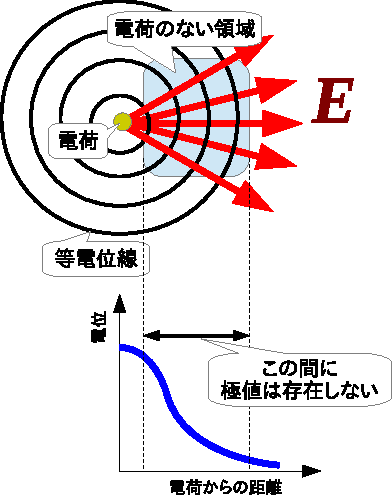
\includegraphics[keepaspectratio, width=6cm,height=7.74cm,clip]{StaticEF_Char1.pdf}
                        \caption{電荷が存在しない領域では,電位は極値をとらない}
                        \label{fig:StaticEF_Char1}
                    \end{center}
                \end{figure}

        \subsubsection{特徴2}\label{subsubsec:char2}
            等電位の閉曲面内に,電荷が存在しない場合,その内部領域全体の電位は,
            閉曲面の電位に等しく,一定である.これも,背理法で説明する.

            閉曲面の内部の電位が一定でない,と仮定する.
            閉曲面が等電位であることから,閉曲面上には電荷は存在しないので,
            この閉曲面の内側に,極値
                \footnote{
                    極値: 極大値あるは極小値のどちらかを指す総称.
                }
            が存在するはずである.
            極値が存在するということは,上記の特徴1の対偶から,
            閉曲面内に電荷が存在するはずである.
                \footnote{
                    特徴1の論理をかいつまむと,「極値が存在しない,ならば,電荷が存在しない」
                    となる.この対偶は,「電荷が存在する,ならば,極値が存在する」である.
                    一般に,「A$\Rightarrow$B」が成立するとき,その対偶「$\lnot$ B $\Rightarrow\lnot$ A」も
                    同時に成立する.
                }.
            しかし,これは,電荷が存在しないという前提に矛盾する.この矛盾は,
            閉曲面内の電位が一定でないという仮定からの帰結である.
            以上から,本特徴2を示せた.
                \begin{figure}[hbt]
                    \begin{center}
                        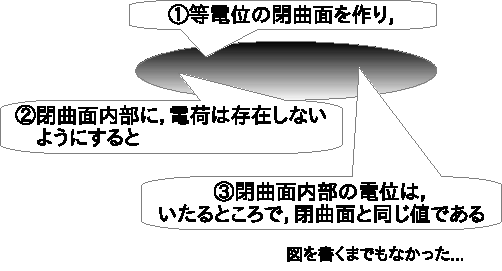
\includegraphics[keepaspectratio, width=6cm,height=5.4cm,clip]{StaticEF_Char2.pdf}
                        \caption{等電位の閉曲面内の電位(内部に電荷を含まず)}
                        \label{fig:StaticEF_Char2}
                    \end{center}
                \end{figure}


        \subsubsection{特徴3}\label{subsubsec:char3}
            任意の閉曲面において,閉曲面の内側の電荷分布と,閉曲面自体の電位が
            与えられれば,その領域内部の電位は,一意に決まる.

%       %==========================================================================
%       %  Subsection
%       %==========================================================================
        \subsection{アーンショーの定理}
        静電場中(ただし,電荷が存在しない領域に限る)では,荷電粒子は安定して存在できる
        位置がない.これを \textbf{アーンショーの定理} という
            \footnote{
                Samuel Earnshaw(1805--1888,イギリス):聖職者で数学者であった人らしい.
            }.
        この定理は,電場に限ったことではなく,磁場でも重力場でも成り立つ.
        距離に関する逆自乗の法則が成り立つならば,この定理が成立する.
                \begin{figure}[hbt]
                    \begin{center}
                        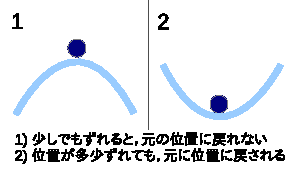
\includegraphics[keepaspectratio, width=5.11cm,height=2.91cm,clip]{Earnshow_000.pdf}
                        \caption{「安定な点」のイメージ}
                        \label{fig:Earnshow_000}
                    \end{center}
                \end{figure}

        実は,この定理は,すでに,上記の静電場の性質として,説明済みである.
        静電場に関するポアソン方程式からの帰結である.上記の性質をただ言い換えた
        だけだけど,この性質には「アーンショーの定理」とも呼ばれる別表現が
        あることを明記しておきたかった.


%   %==========================================================================
%   %  Section
%   %==========================================================================
    \section{導体}
        \begin{mycomment}
            導体といわれると,まず想像するのが,金属だろう.その他にも,
            炭素も有名だ.電解液(イオン溶液)も導体である
                \footnote{
                    ちなみに,純水は電気を通さない.水が電気を通すのは,
                    その中にイオンを含んでいる時のみであり,水道水が電気
                    を通すのも,それが完全な純水ではなく,不純物や塩素な
                    どのイオンを含んでいあるからである.
                }.
            なので,導体と言われても,想像される物質は色々と想像されてしまう.
            そこで,この章で考える導体の範囲に制限を与えることにしよう.
            ここで「導体」とよぶのは,金属や炭素などの個体で,その内部に
            自由電子をもつ物体を指すこととする.イオン溶液は確かに電気を
            通す導体ではあるが,除外する.
        \end{mycomment}

%   %==========================================================================
%   %  Subsection
%   %==========================================================================
    \subsection{導体とは}
        \subsubsection{導体,半導体,絶縁体}
        世の中には,様々な物体がある.石,木,水,葉,$\cdots$など,
        逐一例を上げていったのではきりがないほどだ.そして物体は,
        形,大きさ,硬さ,匂い,色,等,色々など性質をもっている.こういった性質の中で,
        電磁気学で特に興味がある性質に,"電気の通しやすさ" がある.
        電気の通しやすさは,物体を構成する物質そのものや,その構成に左右されるが,
        電磁気学ではそこまで細かいことは考えない
            \footnote{
                ここで学習する電磁気学は,現象論的なものである.
                物性などを含めて考えるときには,より詳細に,微視的
                な電磁気学を学習することも有用だが,内容が高度であるので,割愛する.
            }.
        目で見える範囲の物体を想像すれば十分である.
        とにかく,物体の塊を持ってきて,電気を通すか否かを判別するだけだ.
        物体の種類によって,電気の通しやすさは異なる.極端な例を上げると,
        ゴムは電気を通さないが,金属は電気を通す.様々な物体に対して,
        電気の通しやすさを調べると,それを順に並べることができる
            \footnote{
                電気の通しやすさを測定するには,対象となる物体の大きさを揃えたり,
                周囲の実験環境を揃えたりと,条件を一致させないといけない.
                ここでは,理想的に測ったと仮定しておこう.
            }.
        そうしてできた物体の順列で,電気を通しやすい部分に位置する物体のことを,
        \textbf{導体} という.反対に,電気を通しにくい部分に位置する物体のことは,
        \textbf{不導体} あるいは \textbf{絶縁体} という.
        簡単に言えば,導体とは電気を通しやすい物体のことである.
        また絶縁体は,電気を通しにくい物体のことを指す.

        ここで,"電気を通しやすい?" と表現した理由を説明しておこう
            \footnote{
                こんな回りくどい言い方をしないで,"電気を通す?" と表現したほうが,
                簡潔であると思われるかもしれないので.
            }.
        世の中には,様々な物体が存在するが,不思議な事に,「電気を(完全に)通さない
        物体」は存在しないのである.全ての物体が,電気を通すのである.ゴムなどの
        一般に電気を通さないとされる物体でも,詳細に測定すると,電気が流れることを
        確認できる.ただ,その流れる電気の量が非常に小さいので,電気を通していないと
        みなされるだけなのである.だから,電気を「通す/通さない」ではなく,
        「通しにくい/通しやすい」と書くべきなのである.

        とはいうものの,導体と絶縁体を明確に区別するような基準は存在しない.
        というか,定義すること困難なのである.導体と絶縁体とは,お互いに相対的な
        関係であり,状況によって変わりうるのである.例えば,紙は通常では絶縁体と
        して扱われるが,高電圧を紙にかける場合,電気を通すので,紙は導体として扱
        わないとならない.人間も,乾電池程度の電圧に対しては絶縁体だが,
        家庭用コンセントほどの電圧(100[V])に対しては導体となる
            \footnote{
                電化製品には,感電の恐れがあるという警告が大きく表示されているはず.
                特に,洗濯機において,アース(電気を体に通さないようにする仕組み)は絶対に
                欠かせない.
            }.
        では,導体と絶縁体の区別が全くできない程に曖昧かと
        言われれば,そうではない.\textbf{抵抗} という概念を使えば
            \footnote{
                オームの法則でお馴染みの,抵抗である.
            },
        ある程度区切りを入れることができる.抵抗による区切りも明確ではないが,抵抗は
        電気の通しやすさの1つの指標となる.
        抵抗は,電気物性を考えるときに重要な役割を果たす概念だが,電磁気学の
        理論的枠組を考える場合には,必要ではない
            \footnote{
                しかし,大切なので,後ほど解説をすることになるのだが$\cdots$.
            }.
        さしあたり,導体の例として金属をイメージすれば,十分である.また,
        絶縁体の例は,紙でも石でもゴムでもなんでもいい.
                \begin{figure}[hbt]
                    \begin{center}
                        \includegraphicslarge{DoutaiZetsuentai001.pdf}
                        \caption{導体と絶縁体}
                        \label{fig:DoutaiZetsuentai001}
                    \end{center}
                \end{figure}

        \subsubsection{理想的な導体}
            上記は,現実に存在する導体をイメージして記述した.
            これは,「物性物理学」よりの現実的な導体の説明である.
            しかし,多くの電磁気学の教科書で説明される「導体」は,
            少々異なる.
            電磁気学では,理論を考えやすくするために,理想化された導体を
            用いる.特に浸透している呼び方は無いようなので,
            このノートでは,\textbf{理想的な導体} と表現する.
            理想的な導体が,現実の導体と違う点を,いくつか上げておこう
                \footnote{
                    全部を上げることはできない.というか,思いつく限り上げたところで,
                    それで十分かどうかを判断することができないから.いや,
                    「理想的な導体」を理論的に整合性を保つように定義してやれば,
                    可能なのだけど,興味がない
                    (そんなことに時間をかけたくない,ってのが本音).
                }.
            \begin{myshadebox}{理想的な導体の性質}
                理想的な導体が持つ性質は,次の通り.
                \begin{enumerate}
                    \item 電荷には大きさがない(これは電磁気学全体をとおして同じ)
                    \item 正電荷と負電荷は導体中を自由に移動できる
                    \item 無限に多くの電荷をもっている(電荷の数に上限を与えない)
                    \item 導体中の電荷は,導体の外に出ることはできない
                    \item 連続分布している(原子レベルの不連続状態は考えない)
                \end{enumerate}
            \end{myshadebox}

            考えればいくらでも出てきそうだ
                \footnote{
                    教科書には,大抵の場合,こういった
                    ことは暗黙の了解として,明記されていない.紙面がもったいないからだろうか.
                    まあ,こんな約束なら,読めば簡単に悟れるから書くまでもないか.
                    書き始めるとキリがないし.
                }.
            この辺りで列挙を止めておこう.あとは,気が向いたら追記することにして,
            話をすめよう.

            上記の箇条書きに対して,補足しておきたい.理想的な導体を考える場合,
            それは原子で構成されていると考えてはいけない.確かに,正電荷と負電荷
            を持っているが,正電荷も導体内を自由に移動できるからだ.現実には,
            導体は原子で構成されていて,正電荷は動けない.正電荷も導体内を自由に移動
            できるという点が,はじめは違和感を感じるかもしれない.
                \begin{figure}[hbt]
                    \begin{center}
                        \includegraphicsdefault{risouteki_na_doutai000.pdf}
                        \caption{理想的な導体のイメージ}
                        \label{fig:DoutaiZetsuentai001}
                    \end{center}
                \end{figure}


%   %==========================================================================
%   %  Subsection
%   %==========================================================================
    \subsection{導体と電場の関係}
        \subsubsection{静電誘導}
        電場には,面白い性質がある.導体で囲まれた空間内部には電場は存在不可能
        なのである.導体はその内部に自由電子を含んでいる.この自由電子が,
        導体の外側の電場を打ち消すのである.
        自由電子は,導体中で移動できるため,導体の外側の電場から,
        クーロン力を受ける.自由電子は導体中に多数存在し,
        クーロン力に釣り合うように分布し,静止する.
        こうして静止した自由電子は,導体の外側の電場を完全に打ち消すように
        分布する.

        導体内部の自由電子が,外側の電場によって園分布が変わる現象を,
        \textbf{静電誘導} という.電子が電場に誘導されるイメージ.

        さらに言うと,電場は導体の表面で吸収され,導体中には浸透しない.
        導体内部が空洞だろうとなかろうと,導体の内部では一切電場は発生しない.
                \begin{figure}[hbt]
                    \begin{center}
                        \includegraphicsdefault{Doutai_to_Denba001.pdf}
                        \caption{静電誘導}
                        \label{fig:Doutai_to_Denba001}
                    \end{center}
                \end{figure}


        もちろん,電場を与えた
            \footnote{
                あるいは,電場の状態を変更しても同じこと.
            }
        直後は電荷の移動が起こるため,この間,導体内部にも電場が生じている.
        電荷がどのようにして導体中を移動するかも,興味のあるところだけど,
        ここでは,静電場内の現象を考えたいので,電荷の移動のことは後回し
        にしておこう.ここで考えたいことは,電荷の移動が完了したの,
        導体周辺に生じる静電場である.

        \subsubsection{静電遮蔽}
        上記の静電誘導の見方を変えると,
        導体の内部まで電場が突き抜けることはない,と言っても同じことだ.
        こうした立場からは,この現象を \textbf{静電遮蔽} という
            \footnote{
                あるいは,\textbf{静電シールド} とよばれれることもある.
            }.
        導体が電場を遮蔽するのだ.
                \begin{figure}[hbt]
                    \begin{center}
                        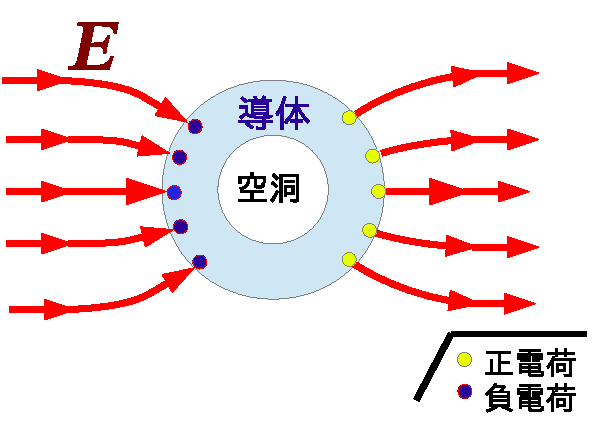
\includegraphics[keepaspectratio, width=6cm,height=4.2cm,clip]{Doutai_to_Denba000.pdf}
                        \caption{静電遮蔽}
                        \label{fig:Doutai_to_Denba000}
                    \end{center}
                \end{figure}

        電場の影響を極力少なくした実験を行う場合,この静電遮蔽が有効である.
        導体に完全に囲まれていれば,その中には電場は侵入してこないのだ.

        \begin{memo}{導体内部に電場は生じない}
            背理法を使って説明しよう(エネルギー保存則との矛盾をつかう).
            もし導体中に電場が発生すると仮定する.
            この時,導体内部の自由電子が,静電誘導を受け移動が始まる.
            しかし,これはエネルギー保存則に反する.なぜなら,
            エネルギーを与えていないにもかかわらず(電場はエネルギーではない),
            電流が生じるはずがないからだ.

            というか,そもそも,導体である条件の1つに,数え切らないくらいの
            自由電子をもっているという性質が要請されていて,電子は電場を吸収する
            のであるから,導体内部に電場が発生しないことは,導体の定義から直接的に
            示されるとも考えられる.
        \end{memo}

        \subsubsection{電場と導体表面}
        電場が導体の表面で吸収される場合,電場は導体表面に直交する.
        導体の形状がどんなに複雑でも,電場は表面に直角に交わる.
                \begin{figure}[hbt]
                    \begin{center}
                        \includegraphicsdefault{Doutai_to_Denba002.pdf}
                        \caption{電場は導体表面に直交する}
                        \label{fig:Doutai_to_Denba002}
                    \end{center}
                \end{figure}

        斜めに交わることはない.もし,斜めに交わってしまうと,導体表面に平行な電場成分が発生する.
        しかし,これは,先に示した導体の性質「導体内部に電場は生じない」と反する.だから,
        道内の内部に電場が生じないように交わるには,直角に交わるしかないのだ.
                \begin{figure}[hbt]
                    \begin{center}
                        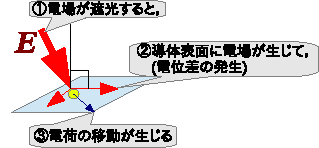
\includegraphics[keepaspectratio, width=6cm,height=2.7cm,clip]{Doutai_to_Denba003.pdf}
                        \caption{もし,電場が導体に直交しなかったら...}
                        \label{fig:Doutai_to_Denba003}
                    \end{center}
                \end{figure}

%   %==========================================================================
%   %  Subsection
%   %==========================================================================
    \subsection{導体と電位の関係}
    導体の表面は等電位面である.導体がどんな形をしていても,等電位面になる.
    電場が導体に垂直に交わることから,簡単に説明できる.
    \ref{subsec:toudeni_denba}節を参照.




%===================================================================================================
%  Chapter : 磁束密度に対するガウスの法則
%  説明    : 磁束密度に対するガウスの法則ビオ・サヴァールの法則から導く
%===================================================================================================
\chapter{磁束密度に対するガウスの法則}
%   %-----------------------------------------------------------------------------------------------
%   %  Input
%   %    File Name : PhysNote_EM_1st_GaussLowBF.tex
%   %-----------------------------------------------------------------------------------------------
        %   %==========================================================================
%   %  Section
%   %==========================================================================
    \section{ビオ$=$サバールの法則(復習)}
        \begin{mycomment}
            ビオ$=$サバールの法則についての詳細は,\ref{subsec:BiotSavart_Gene}節を参照.
            以下は,そこからの抜粋である.
        \end{mycomment}

        ビオ$=$サバールの法則は,磁束密度に関する法則である.
        \begin{myshadebox}{ビオ$=$サバールの法則(電流密度表示)}
            電流はその周囲に磁束密度を発生させる.その発生は以下の式に従う.
            \begin{align}
                \bB(\br)
                = \frac{\mu_{0}}{4\pi}
                    \int \frac{ \bi(\br')\times (\br-\br') }{ |\br-\br'|^{3} } \df V'.
            \end{align}
        \end{myshadebox}
        \begin{figure}[hbt]
            \begin{center}
                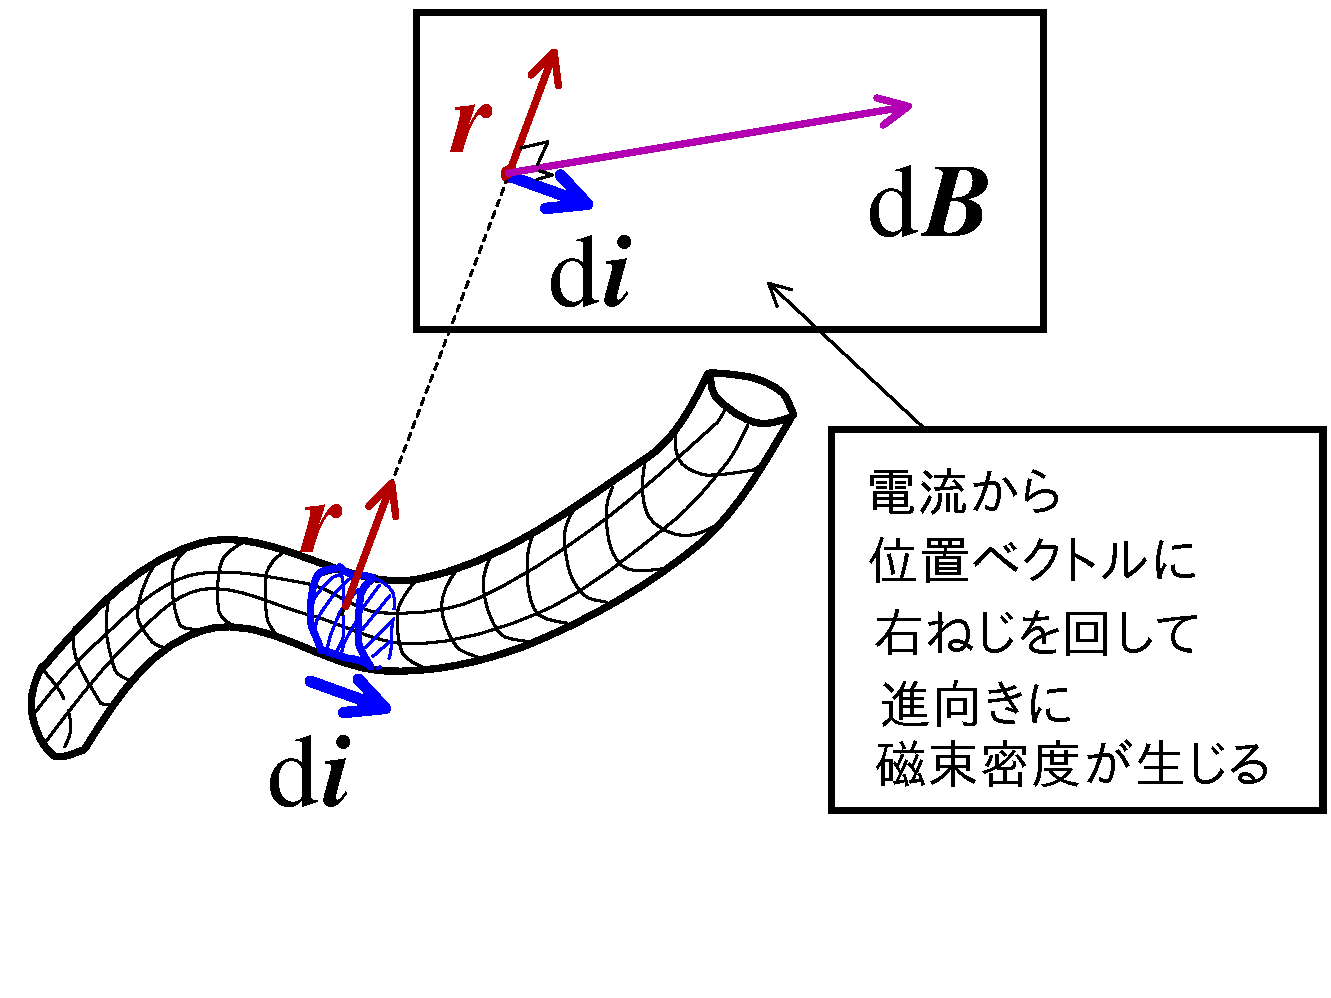
\includegraphics[keepaspectratio, width=7.2cm, height=5.79cm, clip]{biot_savart_1.pdf}
                \caption{ビオ$=$サバールの法則}
            \end{center}
        \end{figure}


%   %==========================================================================
%   %  Section
%   %==========================================================================
    \section{磁束密度に対するガウスの法則の導出}
%   %==========================================================================
%   %  Subsection
%   %==========================================================================
    \subsection{公式の確認}
        ビオ$=$サバールの法則から,磁束密度に対するガウスの法則を導出する
        手順を示す.まず,導出の際に以下のベクトル解析の公式を使用する.
            \begin{align}\label{eq:kousiki_kakunin}
                \dgrad \left( \frac{1}{r} \right) = - \frac{\br}{r^{3}}.  \\
                \drot (a\bX) = (\dgrad a) \times \bX + a(\drot \bX).
            \end{align}
        ただし,$r=\sqrt{x^{2}+y^{2}+z^{2}}$ である.また,$a$ は任意の
        スカラー関数であり,$\bX$ はベクトル関数である.

        \begin{memo}{公式の変形1}
            この公式を使うのだけど,このまま適用するわけではない.
            適用しやすいように,形を変えておこう.上段の式から見ていこう.
                \begin{equation*}
                    \dgrad \left( \frac{1}{r} \right) = - \frac{\br}{r^{3}}.
                \end{equation*}
            の $\br$ に注目する.任意の定ベクトル $\bC$ を考えて,$\br$ を
                \begin{equation*}
                    \br \rightarrow \br - \bC
                \end{equation*}
            と置き換えてやる.すると
                \begin{equation*}
                    \dgrad \left( \frac{1}{|\br - \bC|} \right)
                    =
                    - \frac{\br - \bC}{{|\br - \bC|}^{2}}
                \end{equation*}
            となる
        \footnote{
                    計算は合成微分を繰り返し.面倒だが,$x$ 成分の
                    計算だけでよいので,手で計算してほしい.
                    ここでは,記述が面倒なので,結果のみとする.
                }.
        \end{memo}

        \begin{memo}{公式の変形2}
            任意の定ベクトル $\bX$ に対して,
                \begin{equation*}
                    \drot \bX = \b0
                \end{equation*}
            が成立するとき,
                \begin{equation*}
                    \drot (a\bX) = (\dgrad a) \times \bX
                \end{equation*}
            が成り立つ.
        \end{memo}

%   %==========================================================================
%   %  Subsection
%   %==========================================================================
    \subsection{導出}
        ベクトル解析の公式 $\ddiv (\drot \bX) = 0$ を念頭に置き,
        ビオ$=$サバールの法則の式を変形していこう.

        まず,ビオ$=$サバールの式を書き下す.
            \begin{align}
                \bB(\br)
                =\frac{\mu_{0}}{4\pi}
                \int\frac{\bi(\br')\times
                (\br-\br')
                }{|\br-\br'|^{3}}\df V'.
            \end{align}
        この式の
            \begin{equation*}
                \frac{\br-\br'}{|\br-\br'|^{3}}
            \end{equation*}
        の部分の注目すると,公式
            \begin{equation*}
                \dgrad \left( \frac{1}{|\br - \bC|} \right)
                =
                - \frac{\br - \bC}{{|\br - \bC|}^{2}}
            \end{equation*}
        から
            \begin{align}
                \bB(\br)
                =\frac{\mu_{0}}{4\pi}
                    \int
                        \bi(\br')\times
                            \biggl\{
                                - \dgrad \left( \frac{1}{|\br - \br'} \right)
                            \biggr\}
                    \df V'.
            \end{align}
        さらに,公式($\bU$ は定ベクトル,$a$ はスカラー関数)
            \begin{align*}
                \drot (a\bU) &= (\dgrad a) \times \bU  \\
                             &= -\bU \times (\dgrad a)  \\
                             &= \bU \times (- \dgrad a)
            \end{align*}
        により,
            \begin{align*}
                \bB(\br)
                &=\frac{\mu_{0}}{4\pi}
                    \int
                        \bi(\br')\times
                            \biggl\{
                                - \dgrad \left( \frac{1}{|\br - \br'|} \right)
                            \biggr\}
                    \df V'
                 \\
                &= \int
                        \drot \left( \bi(\br') \frac{1}{|\br - \br'|} \right)
                    \df V'
                 \\
                &= \int
                        \drot \left(\frac{ \bi(\br') }{|\br - \br'|} \right)
                    \df V'.
            \end{align*}
        積分と微分の順番を変更して,
            \begin{align}
                \bB = \drot \int \left(\frac{ \bi(\br') }{|\br - \br'|} \right) \df V'.
            \end{align}

        ここで,次のようなベクトル関数を定義する.
            \begin{align}
                \bA(\br) := \int \frac{ \bi(\br') }{|\br - \br'|} \df V'.
            \end{align}
        これは後で \textbf{ベクトル$\cdot$ポテンシャル} と呼ばれる量と同じものである
            \footnote{
                ここでは,あくまでも形式的に導入するものであり,その正式な導入は後で行う.
            }.
        この $\bA(\br)$ をにより,ビオ$=$サバールの法則は以下のような形になる.
            \begin{align}
                \bB(\br) = \drot \bA(\br).
            \end{align}

        ここまで計算すれば,明らかだ.両辺に $\ddiv$ をとろう.
            \begin{align}
                \ddiv \bB(\br) &= \ddiv \left( \drot \bA(\br) \right). \notag \\
                \therefore \quad
                \ddiv \bB(\br) = 0.
            \end{align}
        この計算で,公式 $\ddiv (\drot \bX) = 0$ を使った.
        これは,磁束密度に対するガウスの法則に他ならない.

        以上の計算から,ビオ$=$サバールの法則に従って生じる磁束密度は,
        ガウスの法則 $\ddiv \bB(\br) = 0$ を満たすことが示された.


%   %==========================================================================
%   %  Subsection
%   %==========================================================================
    \subsection{まとめ}
        以上の結果をまとめよう.
                    \begin{myshadebox}{静磁束密度のガウスの法則(微分形)}
                        時間変化のない磁束密度に対する,局所的な
                        ガウスの法則は,以下の微分形の式により表される.
                        \begin{align}
                            \ddiv \bB =0.
                        \end{align}
                    \end{myshadebox}
                    \begin{myshadebox}{静磁束密度のガウスの法則(積分形)}
                        時間変化のない磁束密度に対する,大局的な
                        ガウスの法則は,以下の積分形の式により表される.
                        \begin{align}
                            \int_{S} \bB(\br) \cdot \bn(\br)\df S=0.
                        \end{align}
                    \end{myshadebox}

            磁束密度に対するガウスの法則は,
            電場に対するガウスの法則
            と同様に考えられる.
            磁束密度に対するガウスの法則
            を表す式を見てみると,
            『任意にとった閉曲面からの磁束密度の
            流出量を積分すると,その値は 0 に
            なる』
            ということ解釈できる.後で確認することではあるが,微分形のマクスウェル方程式によれば,
            磁束密度は,どの場所においても,発生 や 吸い込み がおきていないことがわかる.
            それゆえに,磁束密度の流出も生じないのである.


%   %==========================================================================
%   %  Section
%   %==========================================================================
    \section{法則の意味(図的イメージ)}


%===================================================================================================
%  Chapter : アンペール$=$マクスウェルの法則
%  説明    :
%           1.ビオ$=$サバールの法則から,定常電流のアンペールの法則を導く
%           2.電荷保存則とアンペールの法則の矛盾をのぞくべく,「変位電流」を導入する
%           3.変位電流をアンペールの法則に組み込み,アンペール$=$マクスウェルの法則を導く
%===================================================================================================
\chapter{アンペール$=$マクスウェルの法則}
%   %-----------------------------------------------------------------------------------------------
%   %  Input
%   %    File Name : PhysNote_EM_1st_AMLaw.tex
%   %-----------------------------------------------------------------------------------------------
        %   %==========================================================================
%   %  Section
%   %==========================================================================
    \section{アンペールの法則}
%   %==========================================================================
%   %  Subsection
%   %==========================================================================
    \subsection{エルステッドの実験}
        電流が生じている導体のそばに方位磁針をおくと,方位磁針は南北を示さなくなる.
        エルステッド
            \footnote{
                Hans Christian \O rsted ( 1777 - 1851, デンマーク  ):物理学者,科学者.
                太田光一の著した「電磁気学の基礎\I」には,"エールステズ" と片仮名表記されている.
            }
        はこの現象を発見した.その後,更に多くの実験が行われた.そして,アンペールによって,
        \textbf{アンペール力} (2つの電流の間に生じる力) が発見された.アンペール力 $\bF$ は,
        2つの電流を $I$, $I'$ とし,その間の距離を $l$ としたとき,
            \begin{align}
                \bF = k\frac{II'}{l}
            \end{align}
        で表される.$k$ は比例定数である.$k$ の具体的な数値は後で考えることになる
            \footnote{
                SI単位系において,電流の基本単位1[A] はアンペール力と利用し,定義される.
            }.
        2つの電流の間に,引力もしくは斥力(反発力)が発生するということである.
        2つの電流が同じ方向に向いていれば引力が働く.逆向きであれば,斥力が働く.

        原理を考えてみよう.
        電流の周りには磁束密度が生じる.また,電流とは電荷のいどうのことである.
        一方の電流が作る磁束密度の中を,他方の電流のもとである電荷が移動することになる.
        となれば,電荷は磁束密度中をある速度を持って移動することになるので,
        ローレンツ力を受けることになる.電荷というスケールで考えると,
        ローレンツ力を受けているのであるが,電流という大局的な視点で考えれば,
        アンペール力が働いているのである.アンペール力は原理的にはローレンツ力に
        起因するものと考えても良いが,時と場合によって,使い分けることが大事だ.
        例えば,実験や工学的な目的であればアンペール力を利用したほうが便利だし,
        現象を理論的に追求しようとした場合,ローレンツ力として考えたほうが
        一般性が高まることもあるだろう.

        話がそれたが,この節で言いたかったことは,電流の周囲には磁束密度が生じるという
        ことである.では,具体的には,どのような磁束密度が分布しているのだろうか.
        以下で考えていこう.


%   %==========================================================================
%   %  Subsection
%   %==========================================================================
    \subsection{ビオ$=$サバールの法則(復習)}
        \begin{mycomment}
            ビオ$=$サバールの法則についての詳細は,\ref{subsec:BiotSavart_Gene}節を参照.
            以下は,そこからの抜粋である.
        \end{mycomment}
            \begin{myshadebox}{ビオ$=$サバールの法則(電流密度表示)}
                電流はその周囲に磁束密度を発生させる.その発生は以下の
                式に従う.
                \begin{align}
                    \bB(\br)
                    =\frac{\mu_{0}}{4\pi}
                    \int\frac{\bi(\br')\times
                    (\br-\br')
                    }{|\br-\br'|^{3}}\df V'
                \end{align}
            \end{myshadebox}
            \begin{figure}[hbt]
                \begin{center}
                    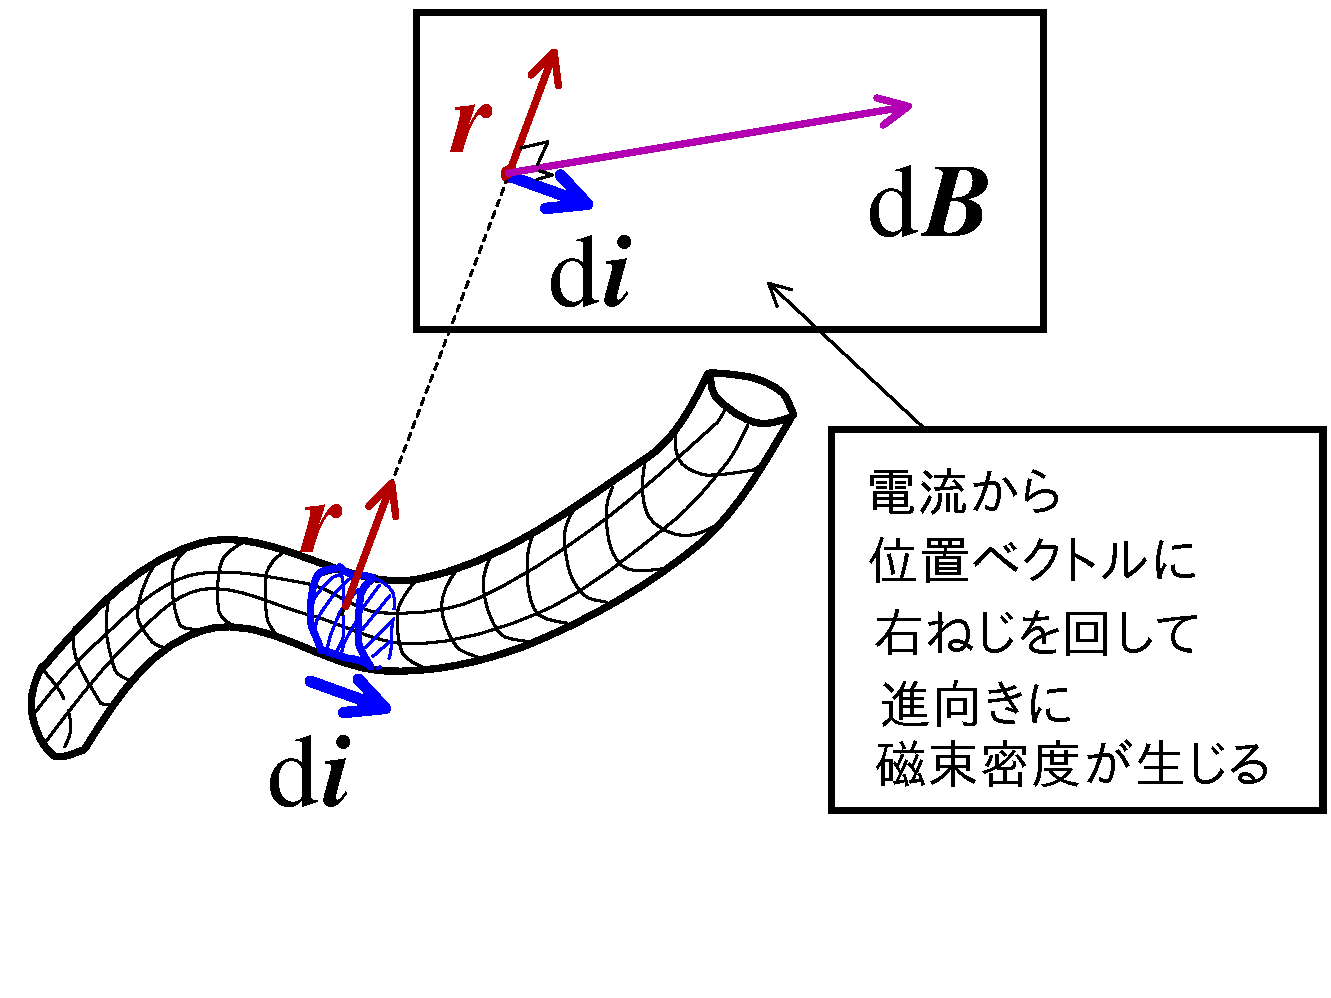
\includegraphics[keepaspectratio, width=7.2cm, height=5.79cm, clip]{biot_savart_1.pdf}
                    \caption{ビオ$=$サバールの法則}
                \end{center}
            \end{figure}

%   %==========================================================================
%   %  Subsection
%   %==========================================================================
    \subsection{アンペールの法則の導出}
%       %======================================================================
%       %  Subsection
%       %======================================================================
        \subsubsection{定常電流}
            ビオ$=$サバールの法則からアンペールの法則を
            導く.はじめに注意しておくと,ビオ$=$サバールの法則は時間変化しない電流
            についての法則である.このような電流を \textbf{定常電流} という.
            従って,以下に導くアンペールの法則も,定常電流を仮定していることになる.
          まず,定常電流を数式で表現しておく.

            電流とは電荷の集団の移動と定義される.電流が時間変化しないということは,
            電荷の移動の時間変化が一定であると考えられる.つまり,電荷密度の
            時間変化はないと解釈できる.ここで,
            電荷保存の法則をおもいだすと,
            \begin{align}
            \frac{\df }{\df t}\int_{\Omega_{S}} \rho(\br,t)\df V
            +\int_{S} \bi(\br,t)\cdot\textit{\textbf{n}}(\br)\df S=0
            \end{align}
            である.電荷密度 $\rho(\br,t)$ が一定の値をとることから,
            この式の第1項は 0 なる.つまり,この式に
            $\frac{\df }{\df t}\int_{\Omega_{S}} \rho(\br,t)\df V=0$ を
            代入して,
            \begin{align}
            \int_{S} \bi(\br,t)\cdot\textit{\textbf{n}}(\br)\df S=0
            \end{align}
            である.この式が定常電流を表現する式である.

%       %======================================================================
%       %  Subsection
%       %======================================================================
        \subsubsection{導出}
            定常電流であることを踏まえてアンペールの法則を導出する.ビオ$=$サバールの法則は
            式(\ref{Bior=savart'slow1})によって,
            \begin{align}
            \bB(\br)
            =\frac{\mu_{0}I}{4\pi}
             \int_{\Gamma}\frac{\bt(\br')\times
             (\br-\br')
            }{|\br-\br'|^{3}}\df s'
            \end{align}
            である.$\bt(\br')\df s'$ とまとめて,
            \begin{align}
            \bB(\br)
            =\frac{\mu_{0}I}{4\pi}
             \int_{\Gamma}\frac{\bt(\br')\df s'\times
             (\br-\br')
            }{|\br-\br'|^{3}}
            \end{align}
            である.
            この式の両辺を曲線 $\Gamma$ を内側に含む閉曲線 $l$ で線積分すると,
            \begin{align}
            &\oint_{l}\bB(\br)\cdot \bt(\br) \df l \notag \\
            &=\frac{\mu_{0}I}{4\pi}\oint_{l}
             \int_{\Gamma}\frac{\bt(\br')\df s'\times
             (\br-\br')
            }{|\br-\br'|^{3}}\cdot \bt^{\ast}(\br)
            \df l
            \end{align}
            とする.ここに,$\bt^{\ast}(\br)\df l$ は 閉曲線 $l$  単位
            接線ベクトル である.この式の右辺に ベクトル解析の公式
            \begin{align*}
            (\bL\times\bM)\cdot\bN
            =(\bN\times\bL)\cdot\bM
            \end{align*}
            を用いると,
            \begin{align}
            &\oint_{l}\bB(\br)\cdot \bt^{\ast}(\br) \df l \notag \\
            &=\frac{\mu_{0}I}{4\pi}\oint_{l}
             \int_{\Gamma}\frac{\bt^{\ast}(\br)\df l\times\bt(\br')\df s'
            }{|\br-\br'|^{3}}\cdot
            (\br-\br')
            \end{align}
            と変形できる.ここで,曲線 $\Gamma$ の単位接線方向ベクトル $\bt(\br')$ と
            閉曲線 $l$ の単位接線成分 $\bt^{\ast}(\br)$ との
            外積 $\bt(\br')\times\bt^{\ast}(\br)$ を
            \begin{align*}
            \textit{\textbf{n}}(\br')=\bt(\br')\times\bt^{\ast}(\br)
            \end{align*}
            とおく.また,$\df S_{l}=\df l\df s'$(「閉曲線 $l$ を縁とする面」という意味)とおく.すると,
            \begin{align}
            \oint_{l}\bB(\br)\cdot \bt^{\ast}(\br)\df l
            =\frac{\mu_{0}I}{4\pi}\oint_{l}
             \int_{S_{l}}\frac{\textit{\textbf{n}}(\br')\df S
            }{|\br-\br'|^{3}}\cdot
            (\br-\br')
            \end{align}
            と書ける.
            さらに曲線 $\Gamma$ が,閉曲線 $l$ の内側にあるので,公式
            \begin{align*}
            &\int_{S_{l}}\frac{\textit{\textbf{n}}(\br')\df S
            }{|\br-\br'|^{3}}\cdot
            (\br-\br') \\
            &=\int_{S_{l}}\frac{\textit{\textbf{n}}(\br')
            }{|\br-\br'|^{3}}\cdot
            (\br-\br')\df S=4\pi
            \end{align*}
            が成り立つ.従って,
            \begin{align}
            \oint_{l}\bB(\br)\cdot \bt^{\ast}(\br)\df l
            =\mu_{0}I
            \end{align}
            となる.この計算では,閉曲線 $l$ の単位接線ベクトルとして,$\bt^{\ast}(\br)$ を
            用いてきたが,ここで改めて,$\bt(\br)=\bt^{\ast}(\br)$ と
            書くことにしても混乱はないので,
            \begin{align}
            \oint_{l}\bB(\br)\cdot \bt(\br)\df l
            =\mu_{0}I
            \end{align}
            さらに,面 $S_{l}$ を流れる電流 を電流密度で表記すると,
            \begin{align}
            I=\int_{S_{l}} \bi(\br)\cdot\textit{\textbf{n}}(\br)\df S_{l}
            \end{align}
            と書けることから
            \footnote{
            この式の $S_{l}$ は閉曲面ではない.$S_{l}$ は
            閉曲線 $l$ を縁とした曲面である. → 電荷保存の法則で考えているのは
            閉曲面 $S$ であって,これとの違いに注意をする.
            },(電流は定常電流である.)
            \begin{align}
            \oint_{l}\bB(\br)\cdot \bt(\br)\df l
            =\mu_{0}\int_{S_{l}} \bi(\br)\cdot\textit{\textbf{n}}(\br)\df S_{l}
            \end{align}
            と表現できる.何度も確認するが,この式の $\bt(\br)$ は
            閉曲線 $l$ の単位接線ベクトルである.
                \begin{myshadebox}{アンペールの法則(積分形)}
                    電流の周囲には磁束密度が生じ,以下の式に従う.
                    \begin{align}
                        \oint_{l} \bB(\br)\cdot\bt(\br)\df l
                        =\mu_{0}\int_{S_{l}} \bi(\br)
                        \cdot\textit{\textbf{n}}(\br)\df S_{l}
                    \end{align}
                \end{myshadebox}

%   %==========================================================================
%   %  Subsection
%   %==========================================================================
    \subsection{法則の意味(図的イメージ)}
        言葉で言えば,「磁束密度 $\bB(\br)$ が
        存在する場所において,任意の閉曲線 $l$ を描き,この閉曲線 $l$ の接線方向に線積分すると,
        その値は閉曲線 $l$ の張る面 $S_{l}$ を貫く電流 $I$ の $\mu_{0}$ 倍に等しい」と言える.
        この式の解釈を簡単にいえば,『電流が磁束密度を生じさせる』ということである.
        つまり,(定常的な)磁束密度が存在するならば,その根源は電流である と言える.

        アンペールの法則を満たす磁束密度は一意に定まらない.そこで,静電場で考えた時と同じように
        磁束密度に対するガウスの法則を導入するのである.このガウスの法則によって,
        磁束密度を一意に決定できるようになる.

%   %==========================================================================
%   %  Section
%   %==========================================================================
    \section{アンペール$=$マクスウェルの法則}
    \begin{mycomment}
        アンペール$=$マクスウェルの法則とは,その記述から察しがつくと
        思うが,アンペールの法則にマクスウェルが改良を加えたものである.
        マクスウェルは,動電磁場を考える場合に,アンペールの法則が不完全
        であるとし,\textbf{変位電流} という新しい概念を導入した.変位電流とは
        なんなのか.マクスウェルはどのように修正したのか.その拡張された
        法則はどういったイメージなのか.この節で考えることにしよう.
    \end{mycomment}

%   %==========================================================================
%   %  Subsection
%   %==========================================================================
    \subsection{アンペールの法則と電荷保存則との矛盾}
        マクスウェルは,アンペールの法則に変位電流の項を加える修正を行った.
        なぜ,このような修正が行われたかというと,アンペールの法則が電荷保存則を
        満たさなかったからである.アンペールの法則は,電荷保存則と矛盾するのだ.
        この矛盾はどういったものなのかを,以下に示す.
            \begin{equation*}
                \drot \bB = \mu_{0}\bi.
            \end{equation*}
        両辺に発散($\ddiv$;divergence)をとってみる.
            \begin{equation*}
                \ddiv( \drot \bB ) = \ddiv ( \mu_{0}\bi ).
            \end{equation*}
        ここで,ベクトル解析の公式から,$\ddiv( \drot \bB ) = 0$ が成立している
            \footnote{
                (公式;定理)任意のベクトル $\bX$ にたいして,
                    \begin{equation*}
                        \ddiv( \drot \bX ) = 0
                    \end{equation*}
                が成立する.
            }.
        つまり,
            \begin{align*}
                \ddiv ( \mu_{0}\bi ) &= 0  \\
                \therefore \quad
                \ddiv \bi &= 0 \,,
                \quad(\because \mu_{0}\mbox{は定数})
            \end{align*}
        となる.ここで,式の見やすさの為に,右辺と左辺を入れ替えた.
        アンペールの法則を認める限り,この式が成立していなければ
        ならないのだけど,一方で,電荷保存則は
            \begin{equation*}
                \ddiv \bi = -\frac{\rd \rho}{\rd t}.
            \end{equation*}
        であり,右辺に関して,$\rd \rho/\rd t \neq 0$ である.
        明らかに,アンペールの法則と電荷保存則は矛盾してしまう.
        どちらが間違っているのだろうか.あるいは,両者とも間違って
        いるのだろうか.マクスウェルの出した答えは,アンペールの法則
        が不完全であるというもので,\textbf{変位電流} という概念を持ち出して,
        修正を加えた.現在では,変位電流の実在性は,電磁波の実験により確固たる
        ものとなっている.

%   %==========================================================================
%   %  Subsection
%   %==========================================================================
    \subsection{変位電流}
        マクスウェルが導入した変位電流とはどのようなものであり,また,
        変位電流の導入はアンペールの法則と電荷保存則の矛盾をどのように解決するか.
        これらを次に確認しよう.
        それには,
        電場に対するガウスの法則に,電荷密度 $\rho$ が現れていることに着目し,
        ここから電荷保存則の式に似せていくという,アプローチをとる.

        電場に対するガウスの法則によれば,
            \begin{align*}
                \ddiv \bE = \frac{1}{\varepsilon_{0}}\rho.
            \end{align*}
        両辺を時間 $t$ で微分する.
            \begin{align*}
                  \frac{\rd}{\rd t}\left(\ddiv \bE \right)
                = \frac{\rd }{\rd t}\left(\frac{1}{\varepsilon_{0}}\rho\right).
            \end{align*}
        ここで,空間に関する微分 $\ddiv$ と時間に関する微分 $\rd/\rd t$ の
        可換性を仮定して
            \footnote{
                時間微分と空間微分は可換であると,信じられている.
                ちなみに,ここに言う「可換」とは,演算の順番のことを言っている.
                つまり,時間微分と空間微分の計算順序を入れ替えてもよい,ということを
                主張している.要は,「空間に関するな微分演算」と「時間」に関する微分演算
                は独立していて,どちらを先に実行しようが,計算結果は変わらないということ.
            },
            \begin{equation*}
                  \ddiv \left(\frac{\rd \bE}{\rd t} \right)
                = \frac{1}{\varepsilon_{0}}\frac{\rd \rho}{\rd t}
            \end{equation*}
        となる.両辺に,$\varepsilon_{0}$ を掛けると,
            \begin{equation*}
                  \ddiv \left(\varepsilon_{0}\frac{\rd \bE}{\rd t} \right)
                = \frac{\rd \rho}{\rd t}.
            \end{equation*}
        最後に,両辺に$-1$をかける.
            \begin{equation*}
                  \ddiv \left( - \varepsilon_{0}\frac{\rd \bE}{\rd t} \right)
                = - \frac{\rd \rho}{\rd t}.
            \end{equation*}
        ここで,再度,電荷保存則の式を見てみよう.
            \begin{equation*}
                \ddiv \bi = -\frac{\rd \rho}{\rd t}.
            \end{equation*}

        電荷保存則と見比べてみると,$- \varepsilon_{0}(\rd \bE/\rd t)$ が
        電流密度と同じ働きをすることが見て取れる.しかし,この項は電流密度そ
        のものを表しているのではない事に注意しよう.
        この項 $\varepsilon_{0}(\rd \bE/\rd t)$ は \textbf{変位電流} とよばれる.

        電場の時間変化 $- \varepsilon_{0}(\rd \bE/\rd t)$ が,電流のように振る舞うように見える.
        考察している範囲に電荷密度が存在していなくとも,電場の時間変化が生じていれば,それを
        電流とみなして良いことを示唆していそうだ.
        アンペールの法則と電荷保存則との矛盾を解く鍵だと言っていい.
        実際にマクスウェルはこの項を持ち出して,アンペールの法則に手を加えて,矛盾を解消した.

%   %==========================================================================
%   %  Subsection
%   %==========================================================================
    \subsection{アンペール$=$マクスウェルの法則の導出}
        アンペール$=$マクスウェルの法則とは,前にも書いた通り,
        アンペールの法則に変位電流の考えを加えたものである.
        その方程式を先に書いてみれば,
        \begin{align}
            \drot \bB
                =   \mu_{0} \bi
                  + \varepsilon_{0} \mu_{0} \frac{\rd \bE}{\rd t}.
        \end{align}
        この方程式は,アンペールにより発見された \textbf{アンペールの法則} に,
        マクスウェルが修正を加えたもので,\textbf{アンペール$=$マクスウェルの法則} と
        よばれる.

        式の形を見るとは,単に,アンペールの法則の右辺に,
        変位電流を加えただけだ.しかし,電荷保存則との矛盾が解消されている.
        右辺第二項の $\varepsilon_{0} \mu_{0} (\rd \bE/\rd t)$ が
        あるため,$\ddiv \bi=0$ となっても,
                \begin{equation*}
            \drot \bB = \varepsilon_{0} \mu_{0} \frac{\rd \bE}{\rd t}.
                \end{equation*}
        となって,電荷保存則と矛盾はしない.
        この式を解釈すると,電場の時間変化が回転する磁場を発生させる,
        ということになる.

%   %==========================================================================
%   %  Subsection
%   %==========================================================================
    \subsection{法則の意味(図的イメージ)}

%   %==========================================================================
%   %  Section
%   %==========================================================================
    \section{静電容量}
%   %==========================================================================
%   %  Subsection
%   %==========================================================================
    \subsection{キャパシタンス}

    \begin{memo}{「キャパシタ」と「キャパシタンス」の違い}
    \end{memo}

%   %==========================================================================
%   %  Subsection
%   %==========================================================================
    \subsection{変位電流とキャパシタ}

%   %==========================================================================
%   %  Subsection
%   %==========================================================================
    \subsection{平行平板型のキャパシタ}

%   %==========================================================================
%   %  Section
%   %==========================================================================
    \section{電流のSI単位に基づく定義}
%   %==========================================================================
%   %  Subsection
%   %==========================================================================
    \subsection{直線電流が作る磁束密度}
        さて,今まで電流の単位として [A]=[C・s] を用いてきたが,
        先にも書いたように,これは現実の定義とは違うものである.
        SI単位系における基本単位は,電荷ではなく,電流が
        採用されている.

        今までの議論で電流を定義するための準備
        ができたので,そのための準備としてのこの項目と,次も項目で,
        電流の定義をし直すことにする.

        まず,定義の概略を示しておく.電流は電荷の移動によって生じる現象であるので,
        電流はローレンツ力を受ける.この電流に対するローレンツ力を人間が観測する
        するときは,導線が受ける力として観測される.
        その力は $\bF=\textit{\textbf{I}}\times \bB$ で表現できた.
        ここで,2つの平行な直線の導線を用意する.この2つの導線に同じ向きに電流を流すと,後に示すように,
        導線が互いに引き合う現象が生じる
        \footnote{
            電流を逆向きに流せば,導線同士は互いに反発しあう.
        }
        .この力によって電流を定義するのである.実際の力の大きさとしては $2\times 10^{-7}$ [N/m] が
        採用されている.
        導線同士が互いに引き合うのはローレンツ力によるものであり,これは
        一方の電流の作る磁束密度が,他方の電流(電荷)に及ぼすローレンツ力である.
        従って,1つの導線に流れる電流が作る磁束密度を計算する必要があり,
        ここではその計算をすることが目的である.そして,次の項目でここでの計算結果を
        利用して,電流を定義していこうと考える.

        直線電流が図\ref{fig:den_jisoku}のような磁束密度を作ることを確認する.
        1本の直線な導線を用意する.この導線に定常電流 $\textit{\textit{i}}$ を流し,
        この定常電流がその周囲に作る磁束密度を考える.
        アンペールの法則は
                    \begin{align}
                        \oint_{l} \bB(\br)\cdot\bt(\br)\df l
                        =\mu_{0}\int_{S_{l}} \bi(\br)
                        \cdot\textit{\textbf{n}}(\br)\df S_{l}
                    \end{align}
        のように書かれる.
            \begin{figure}[hbt]
                \begin{tabular}{cc}
                    \begin{minipage}{0.5\hsize}
                \begin{center}
                    \includegraphicsdouble{den_jisoku.pdf}
                    \caption{電流の作る磁束密度}
                    \label{fig:den_jisoku}
                \end{center}
                    \end{minipage}
                    \begin{minipage}{0.5\hsize}
                \begin{center}
                    \includegraphicsdouble{den_lorentz.pdf}
                    \caption{電荷の磁束密度から受けるローレンツ力}
                    \label{fig:den_lorentz}
                \end{center}
                    \end{minipage}
                \end{tabular}
            \end{figure}

        磁束密度の大きさは,ビオ$=$サバールの法則から,
        導線から等距離にある部分では等しくならないといけない.
        従って,直線の導線の任意の点を流れる電流が起こす,磁束密度の
        大きさが等しい部分をつないでいけば,その形は閉じた
        円になる.そして磁束密度の向きは電流の生じる方向に対して
        右回りである.図\ref{fig:den_lorentz}参照.これがわかれば,
        アンペールの法則の左辺;$\oint_{l} \bB(\br)\cdot\bt(\br)\df l$ の
        積分経路は,円にとればよいことがわかる.

        積分経路を円とすれば,その半径を $r$ とした場合に,
        磁束密度の強さは,以下のように計算される.

        アンペールの法則の左辺を計算すると,
            \begin{align*}
                \mbox{(左辺)}=\oint_{l} \bB(\br)\cdot\bt(\br)\df l
                      =\oint_{l}B\,\df l=B\oint_{l}\,\df l
            \end{align*}
        ここで,積分経路 $l$ は円であるので,$\oint_{l}\,\df l=2\pi r$ である.従って,
            \begin{align*}
                \mbox{(左辺)}=2\pi rB
            \end{align*}
        右辺;$\mu_{0}\int_{S_{l}} \bi(\br)\cdot\textit{\textbf{n}}(\br)\df S_{l}$ は,
        定常電流であるので,これは $\mu_{0}I$ と書ける.

        以上から
            \begin{align*}
                2\pi rB=\mu_{0}I
            \end{align*}
        すなわち,
            \begin{align}
                B=\frac{\mu_{0}I}{2\pi r}
            \end{align}
        である.

        \begin{memo}{積分経路を円にとる}
            なぜなら,円でない曲線経路を
            とったとしても,磁束密度の向きは円方向を向いているからである.
            下図参照.
                \begin{figure}[hbt]
                    \begin{center}
                        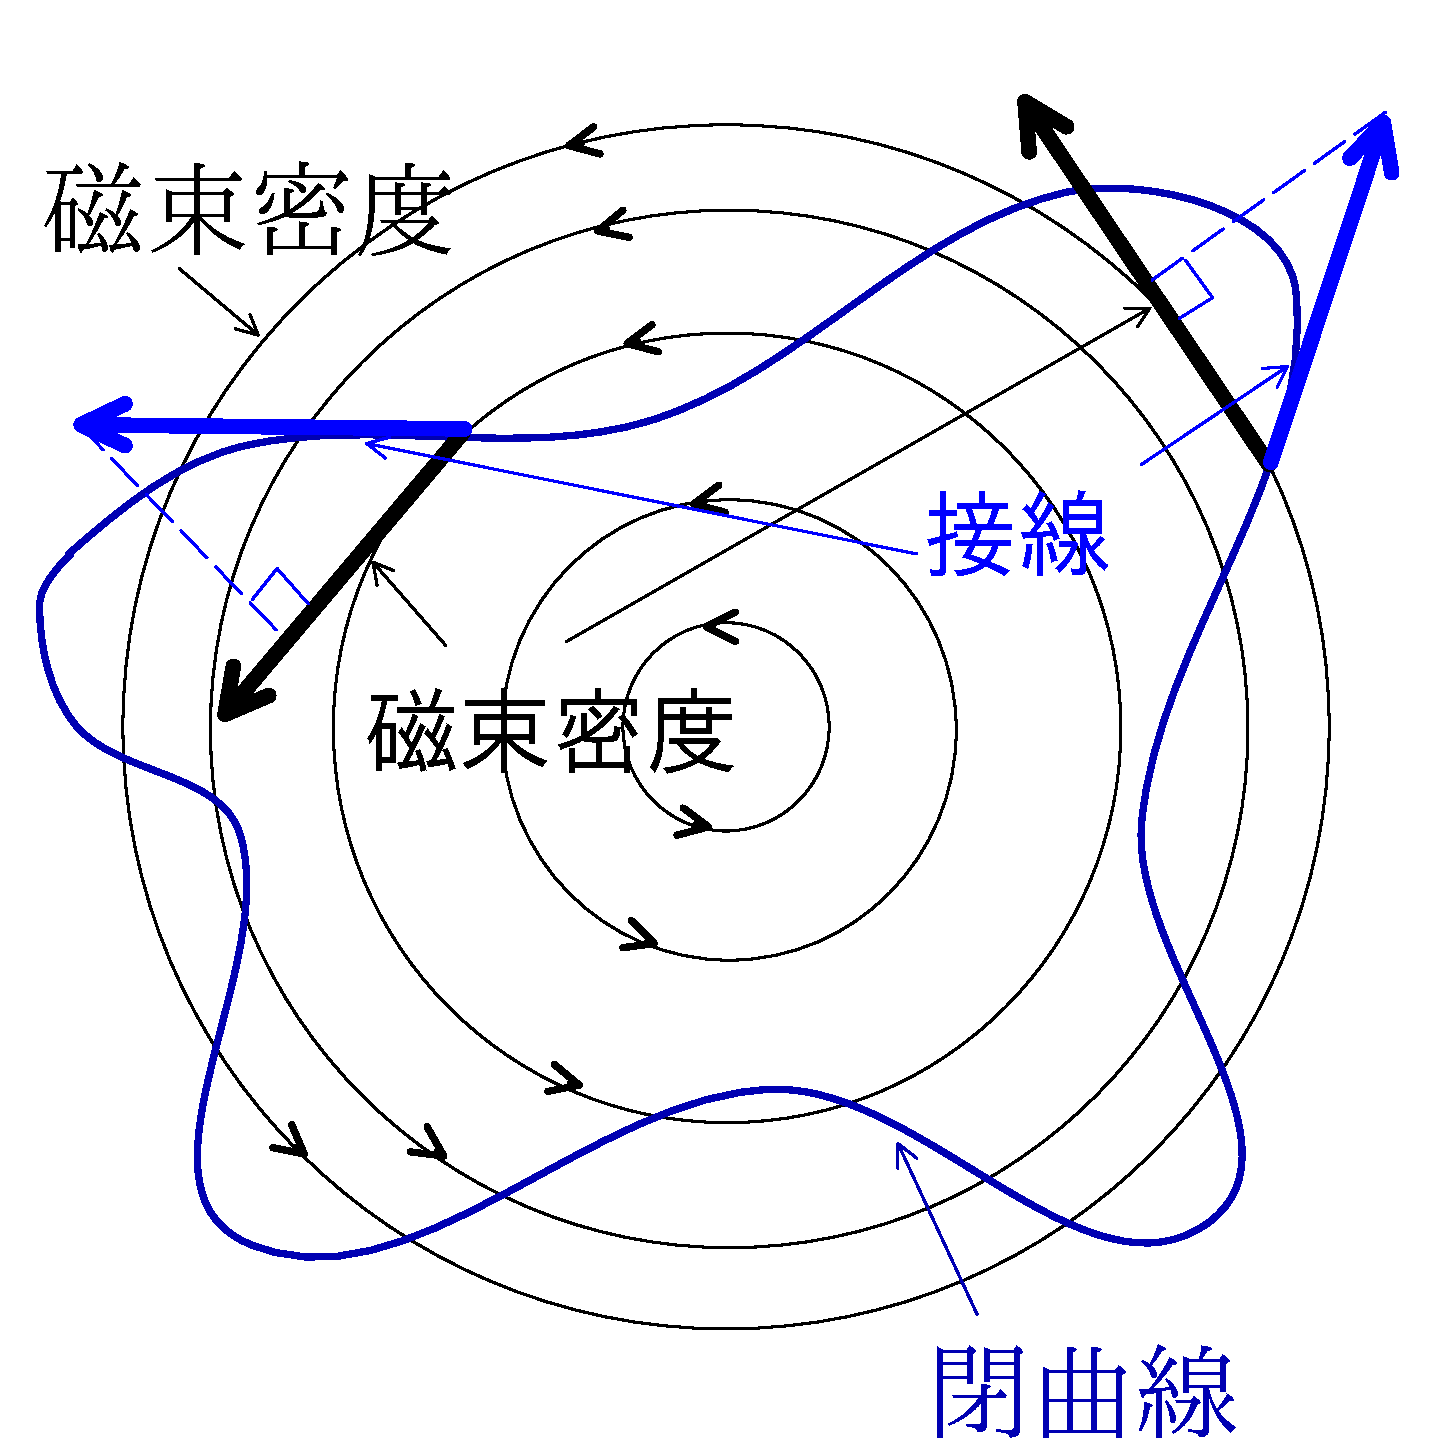
\includegraphics[keepaspectratio, width=6cm,height=6cm,clip]{dentei1.pdf}
                        \caption{閉曲線の取り方}
                        \label{fig:dentei1}
                    \end{center}
                \end{figure}

            図で示したように,曲線の接線と磁束密度の内積をとるので,
            接線の磁束密度に直角な方向成分は考察する必要がないのである.
            (考えたとしても,内積は0となるので意味がない.)
        \end{memo}

%   %==========================================================================
%   %  Subsection
%   %==========================================================================
    \subsection{電流が受ける力}
            電気量 $q$,速度 $\bv$  をもつ1つの電荷が受けるローレンツ力 $\bF$ をおもいだすと,
            \begin{align}
            \bF=q\bv\times\bB
            \end{align}
            であった.
            複数の電荷を考えれば,電荷密度という概念を導入して,
            \begin{align}
            \bF=\left(\int_\Omega \rho(\br)\df V\right)
            \langle\dot{\br}\rangle\times\bB
            \end{align}
            ここに,$\langle\dot{\br}\rangle$ は電荷のドリフト速度である.
            ドリフト速度というのは,複数の電荷の移動速度の平均である.
            そして,$Q:=\int_\Omega \rho(\br)\df V$ おくと,
            $\bF=Q
            \langle\dot{\br}\rangle\times\bB$ と書けて,
            $Q\langle\dot{\br}\rangle$ は電流を表現していると考えられるから,
            これを $\textit{\textbf{I}}$ おくことで($\textit{\textbf{I}}:= Q\langle\dot{\br}\rangle$),
            \begin{align}
            \bF=\textit{\textbf{I}}\times\bB
            \end{align}
            を得る.

%   %==========================================================================
%   %  Subsection
%   %==========================================================================
    \subsection{電流の定義(1[A]の定義)}\label{denryuuteigi}
            電磁気学ではSI単位系において,電流の単位が基本単位として
            採用されている.ここではその基本単位となる電流の1[A]を
            定義する.一つ前の項目\ref{dennryuunoukerutikara}で
            電流が受ける力は,導線の受ける力として現れることを確認し,
            その力は式(\ref{denruu_F})で表された.それをもう一度
            書き下せば,
                \begin{align}
                    \bF=\textit{\textbf{I}}\times \bB
                \end{align}
            である.
            \begin{figure}[hbt]
                    \begin{center}
                        \includegraphicsdefault{denryu_teigi.pdf}
                        \caption{電流の定義の説明図1}
                        \label{fig:denryu_teigi}
                    \end{center}
                \end{figure}

            2本の平行に並んだ導線を用意する.導線の名前をそれぞれ1,2とする.
            この2本の導線に定常電流を流す.それら2つの定常電流を
            それぞれ $\textit{\textit{i}}_{A}$,$\textit{\textit{i}}_{B}$ と
            する.この内の一方の導線に流れる電流が作る磁束密度を考える.
            どちらでもよいが $\textit{\textit{i}}_{1}$ の作る磁束密度を考える.
            アンペールの法則より,
                \begin{align*}
                    \oint_{l} \bB(\br)\cdot\bt(\br)\df l
                    =\mu_{0}\int_{S_{l}} \bi_{1}(\br)
                    \cdot\textit{\textbf{n}}(\br)\df S_{l}
                \end{align*}
            これは前項目で計算計算したように,
                \begin{align*}
                    B=\frac{\mu_{0}I_{1}}{2\pi r}
                \end{align*}
            である.従って,他方の導線に与える力は,
            (電流と磁束密度のなす角は $\pi/2$ であることに注意して)
                \begin{align*}
                    F=I_{2}B\sin\frac{\pi}{2}=I_{2}B
                \end{align*}
            従って,$B=\mu_{0}I_{1}/2\pi r$ を代入すれば.
                \begin{align}
                F=\frac{\mu_{0}I_{1}I_{2}}{2\pi r}
                \end{align}
            である.
            この式を用いて1[A]の電流を定義する.図\ref{fig:AARA}に描いたように,
            重さ $2\times10^{-7}$[N] のおもりを,同線の片方につるす.
                \begin{figure}[hbt]
                    \begin{center}
                        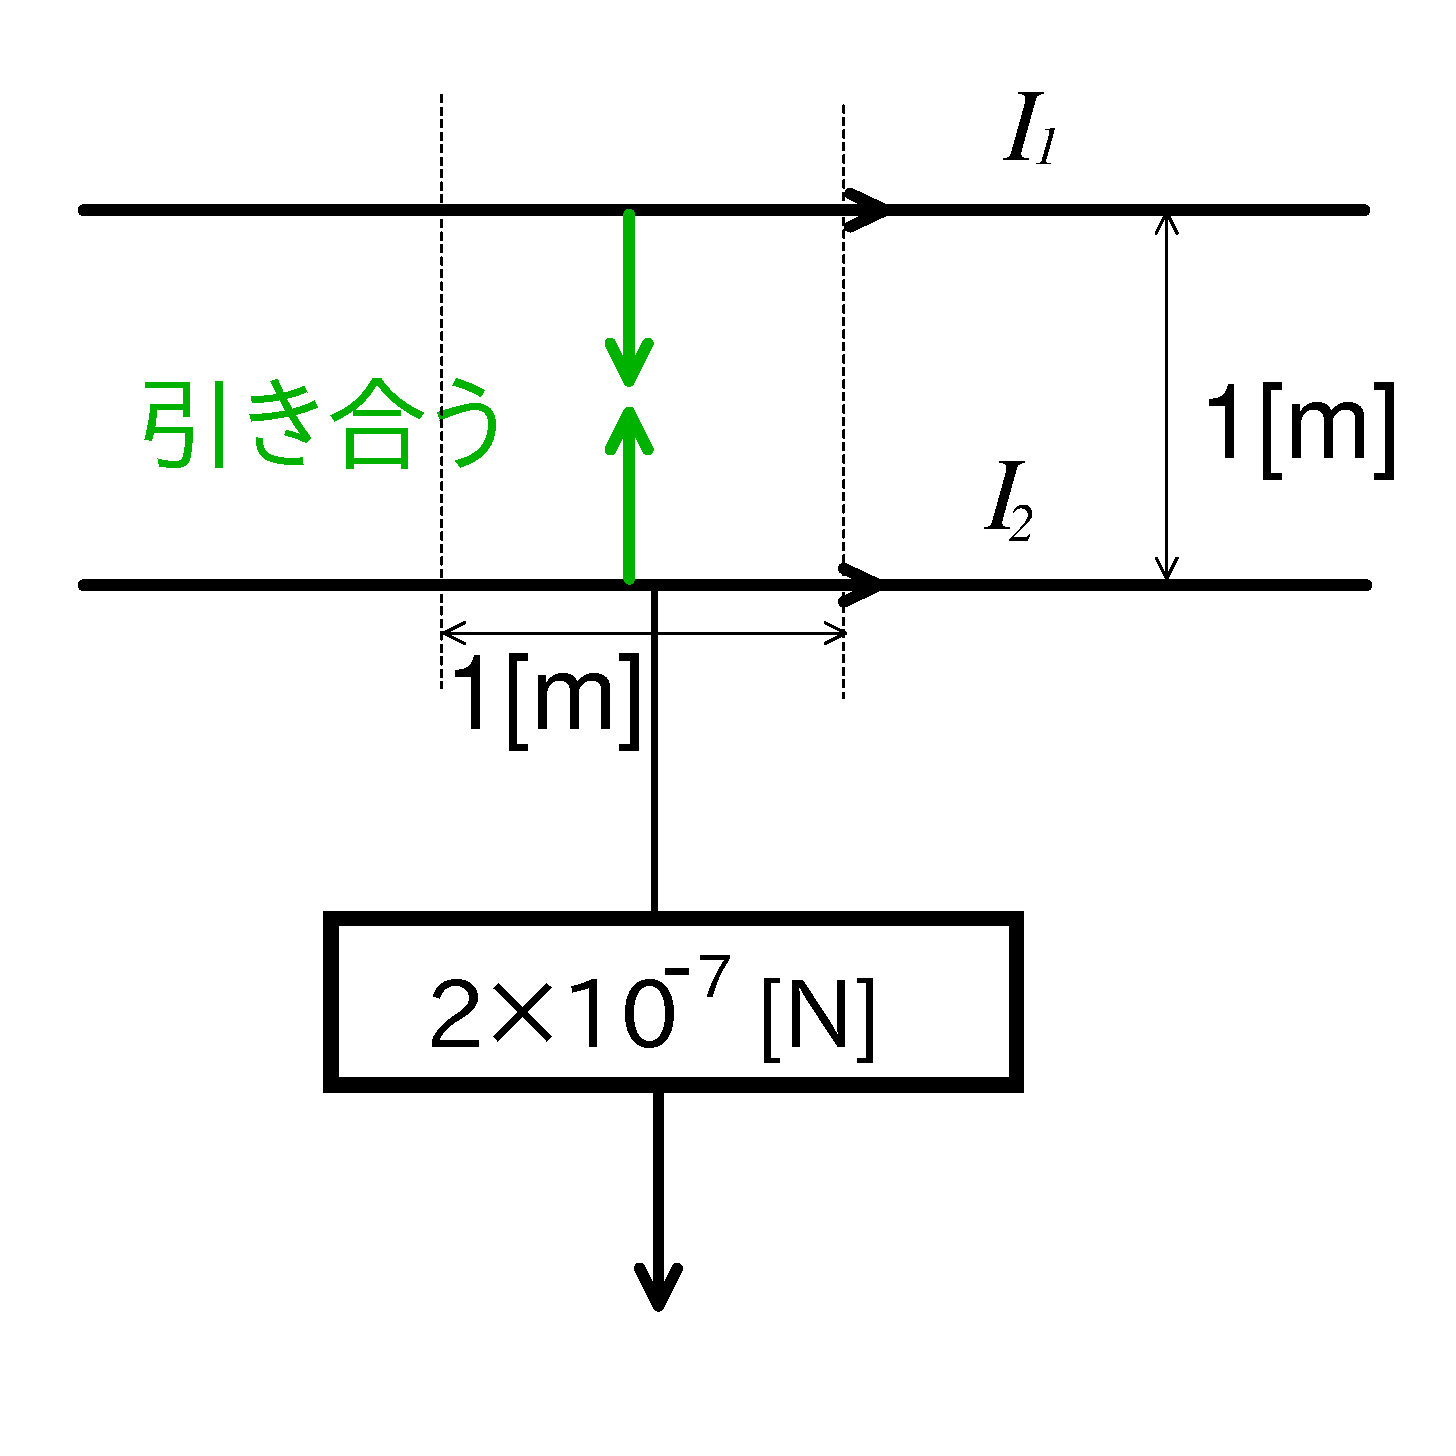
\includegraphics[keepaspectratio, width=5cm,height=4.5cm,clip]{AARA.pdf}
                        \caption{電流の定義の説明図2}
                        \label{fig:AARA}
                    \end{center}
                \end{figure}

            このとき,各導線には同じ方向に電流が流れているとする.
            導線間の距離は1[m]としている.
            この状態で,釣り合いが取れたとき,1[A]の電流が流れていると
            定義するのである.

            以上のことを形式的にまとめておこう.
                \begin{myshadebox}{電流1[A]の定義}
                    1[m]の間隔をおいた
                    2本の平行導線に電流を流して,
                    この導線に働く力が単位長さ(1[m])当たり $2\times10^{-7}$[N] の
                    力が働くとき,
                    この時に流れる電流を1[A]
                    と定義する.
                \end{myshadebox}


%===================================================================================================
%  Chapter : ファラデーの電磁誘導の法則
%  説明    :
%           1.ビオ$=$サバールの法則から,定常電流のアンペールの法則を導く
%           2.電荷保存則とアンペールの法則の矛盾をのぞくべく,「変位電流」を導入する
%           3.変位電流をアンペールの法則に組み込み,アンペール$=$マクスウェルの法則を導く
%===================================================================================================
\chapter{ファラデーの電磁誘導の法則}
%   %-----------------------------------------------------------------------------------------------
%   %  Input
%   %    File Name : PhysNote_EM_1st_EInduction.tex
%   %-----------------------------------------------------------------------------------------------
        %   %==========================================================================
%   %  Section
%   %==========================================================================
    \section{ファラデーの実験}
%   %==========================================================================
%   %  Subsection
%   %==========================================================================
    \subsection{起電力}
        「起電力」とは電流を発生させるためのエネルギー源である.
        具体的には 電池 と考えてよい.とにかく,電流を発生させる
        ものである.実際は,電流は電荷の移動であるので,従って,
        「起電力」とは電荷を動かすものである.電荷を動かすものと
        いえば,電場である.すなわち,起電力とは電場を導体内に発
        生させるエネルギー源であると言える.エネルギーと仕事の関
        係から,起電力は「導体内において,単位電荷を周させる仕事
        」と考えられる.従って,起電力を $V_{l}$ と書くと,(回路
        として閉ループ $l$ を想定するために,このような添え字を
        つけた.)
            \begin{align}
                V_{l}=\oint_{l} \bE(\br,t)\cdot\bt(\br,t) \,\df l
            \end{align}
        なる関係式を得ることができる.以後,\textbf{起電力} とは
        この $V_{l}$ のこという.


%   %==========================================================================
%   %  Subsection
%   %==========================================================================
    \subsection{磁束}
        イメージを先に書くと,「磁束蜜度の束」である.
        これは以下のように表現される.磁束密度を
        閉ループ $l$ を縁とする面 $S_{l}$ で面積分して,
            \begin{align}
                \Phi_{l}=\int_{S_{l}} \bB(\br,t)
                \cdot\textit{\textbf{n}}(\br,t) \,\df S_{l}
            \end{align}
        である.この $\Phi_l{}$ を \textbf{磁束} という.
            \begin{figure}[hbt]
                \begin{center}
                    \includegraphicsdefault{jisoku_image.pdf}
                    \caption{磁束のイメージ}
                    \label{fig:jisoku_image}
                \end{center}
            \end{figure}

%   %==========================================================================
%   %  Subsection
%   %==========================================================================
    \subsection{電磁誘導の法則}
            前にもビオ$=$サバールの法則の部分で書いたが,エルステッドは電流が生じるとそ
            の周りには磁束密度ができることを発見した
                \footnote{
                    電流を流している導線の近くに,方位磁針をいくつか置いてみると,
                    方位磁針は電流の作る磁束密度の方向に振れる.
                }.
            この現象はビオ$=$サバールの法則によって数学的に表現され,さらに,
            アンペールの法則と磁束密度に対するガウスの法則に形を変えている.

            ファラデーは電流が磁束密度を作るのならば,その逆作用として,磁束密度の
            中に置いた回路に電流が生じるのではないかと考えた.その実験の中で,彼
            は磁束密度の時間変化が電場を発生させることを発見した.そして,ノイマン
                \footnote{
                    Frantz Ernst Neumann:(1798 - 1895, ドイツの物理学者,鉱物学者)
                }
            は,この電磁誘導の法則を次のように定式化した.\\
                \begin{center}
                    \begin{itembox}[l]{\textbf{ファラデーの電磁誘導の法則}}
                        閉曲線 $l$ が張る曲面 $S_{l}$ を貫く磁束 $\Phi_{l}$ が時間変化すると,
                        この閉路 $l$ に起電力 $V_{l}$ が生じる.
                        この起電力 $V_{l}$ の大きさは,磁束 $\Phi_{l}$ の
                        時間変化率$\rd \Phi_{l}/\rd t$ に比例する.
                        また,起電力 $V_{l}$ の向きは,
                        この起電力によって閉路 $l$ に電流が生じるときに,
                        この電流が作る磁束がはじめの
                        磁束の変化を打ち消すような向きである.
                        起電力の向きに関すること
                        は \textbf{レンツの法則} とよばれる.
                        磁束 $\Phi_{l}$ の時間変化による閉路 $l$ 内に
                        生じる起電力 $V_{l}$ を,\textbf{誘導起電力} という.
                        ファラデーの電磁誘導の法則は,次式によって表される.
                        \begin{align}\label{denjiyudo}
                        V_{l}=-\frac{\rd \Phi_{l}}{\rd t}
                        \end{align}
                        誘導起電力によって回路に電流が生じるときに,
                        この電流が作る磁束がはじめの磁束の変化のきを正の向きとした.
                    \end{itembox}
                \end{center}

%   %==========================================================================
%   %  Subsection
%   %==========================================================================
    \subsection{法則の意味(図的イメージ)}
                電磁誘導の最も直感的なイメージを図\ref{fig:denjiyuudou},\ref{fig:denjiyuudou3}に示す
                    \footnote{図\ref{fig:denjiyuudou3}は
                        \url{http://vanity-worth.com/nature-law/lenz-1.htm}より(2008.08.24現在).
                    }.
                磁石が振動することによって,その磁石から生じている磁束が
                時間変化することになる.従って,この磁束密度の時間変化により,
                電場が生じることになる.もし,振動している磁石の周りに回路があるならば,
                回路の導線内には電場が生じ,従って起電力となる.
            \begin{figure}[hbt]
                    \begin{center}
                        \includegraphicsdefault{dennjiyuudou.pdf}
                        \caption{電磁誘導1-1}
                        \label{fig:denjiyuudou}
                    \end{center}
            \end{figure}
            \begin{figure}[hbt]
                    \begin{center}
                        \includegraphicsdefault{dennjiyuudou3.pdf}
                        \caption{電磁誘導1-2}
                        \label{fig:denjiyuudou3}
                    \end{center}
            \end{figure}

            電磁誘導の法則を別のイメージで考えてみる.原理は同じだが,次の例は
            とても面白い現象が得られる.

            コイルに電流を流すと磁束密度が生じることは,アンペールの法則から説明される.
            そこで,互いに近くに置かれた
            コイルを2つ用意し,片方(コイル1)にスイッチと電源を接続して,もう一方(コイル2)には
            何も接続しないようにする.図\ref{fig:denjiyuudou2}参照.

            まず初めの状態として,コイル1が電源に接続されスイッチが切れいている状態にする.
            このときはコイル1に電流が流れて得ておらず,従って,コイル1には磁束密度は
            生じていない.この状態からスイッチを入れてコイル1に電流を流してみると,
            この電流によってコイル1に電流が生じる.この電流は磁束密度を発生させる.
            つまり,コイル1の周りに「磁束密度の変化」があったことになる.
            ファラデーの電磁誘導の法則は,磁束密度の変化が回転する電場を生じさせるという
            ものであったので,
            この磁束密度の変化がコイル2の部分においても生じているはずであり,
            従って,コイル2に回転する電場が生じるはずである.つまり,
            コイル2に電流が生じるのである(電源がつながれていないのにもかかわらず!!).
                \begin{figure}[hbt]
                    \begin{center}
                        \includegraphicsdefault{dennjiyuudou2.pdf}
                        \caption{電磁誘導2}
                        \label{fig:denjiyuudou2}
                    \end{center}
                \end{figure}

            電磁誘導の法則(\ref{denjiyudo})を 電場 と 磁束密度 を用いて
            表現すれば,起電力 と 磁束 の項目から,次のように表現できる.
                    \begin{myshadebox}\textbf{ファラデーの電磁誘導の法則}
                        \begin{align}
                        \oint_{l} \bE\cdot\bt \,\df l =-\frac{\rd}{\rd t}\int_{S_{l}} \bB \cdot\textit{\textbf{n}} \,\df S_{l}
                        \end{align}
                        ここに,$\bE:=\bE(\br,t)$,$\bt:=\bt(\br,t)$,$\bB:=\bB(\br,t)$,$\bn:=\textit{\textbf{n}}(\br,t)$ であり,
                        位置と時間の関数である.これらが時間依存している点が重要である.
                        時間依存していなければ右辺は定数となり,静電場の方程式となる
                            \footnote{
                                この意味で,ファラデーの電磁誘導の法則は,静電場の方程式の
                                時間依存的な拡張と見ることもできる.
                            }.
                    \end{myshadebox}

%   %==========================================================================
%   %  section
%   %==========================================================================
    \section{自己誘導 / 相互誘導}
%   %==========================================================================
%   %  Subsection
%   %==========================================================================
    \subsection{自己インダクタンス}
        アンペールの法則によると,磁束密度 $B$ は電流 $I$ に比例する.
        先に見たとおり,磁束 $\Phi$ は 磁束密度 $B$ に比例するので
            \footnote{
                そのように,磁束を定義したのであった.
            },
        当然,\textbf{磁束は電流に比例する}.
            \begin{equation*}
               \Phi \propto B \propto I.
            \end{equation*}
        従って,磁束 $\Phi$ と電流 $I$ の関係式は,
        比例定数を $L$ としたときに,
            \begin{equation*}
                \Phi = LI.
            \end{equation*}
        これを電磁誘導の法則 $V=-\df \Phi/\df t$ に代入すると,
            \begin{align}
                V=-\frac{\df \Phi}{\df t}
                 =-L\frac{\df I}{\df t}
            \end{align}
        となる.この定数 $L$ を \textbf{自己インダクタンス} とよぶ.

        物理的イメージを考えてみよう.アンペールの法則により,電流は
        その周囲に磁束密度を発生させる.一方で,電磁誘導の法則によれば,
        時間変化する磁束密度の周囲には,電場が生じ,電位差が発生する.
        とすると,電流が流れていなかった導線に,突然に電流が流れ始めると,
        その周囲に磁束密度が発生するのだが,この磁束密度は時間変化するものであるので,
        同時に電位差もその周囲に生まれることになる.当然,いま流れ始めた電流は
        この電位差の影響もうけることになる.電流自身がその周囲に電位差を作り出し,
        その電位差が自身に帰ってくるのである."自己"インダクタンスと表現されている
        のは,この現象に由来している.

        \begin{memo}{磁束は電流に比例する}
            以下のように,簡略表記すると,わかりやすい.
            一重巻きのコイルを想定してみればよい.
            積分形のアンペールの法則は
            \begin{equation*}
                \oint_{l} \bB(\br)\cdot\bt(\br)\df l
                =\mu_{0}\int_{S_{l}} \bi(\br)
                \cdot\textit{\textbf{n}}(\br)\df S_{l}
            \end{equation*}
            であるから,
            \begin{equation*}
                B = \oint_{l} \bB(\br)\cdot\bt(\br)\df l
            \end{equation*}
            \begin{equation*}
                I = \int_{S_{l}} \bi(\br)\cdot\textit{\textbf{n}}(\br)\df S_{l}
            \end{equation*}
            と計算されたとき,
            \begin{equation*}
                B=\mu_{0}I.
            \end{equation*}
        \end{memo}

        \begin{memo}{ソレノイドが作る磁束密度}
            ソレノイド上の導線が作る磁束密度を考えよう.
            いま,ソレノイドを流れる電流 $I$ が定常状態であるとしたとき,アンペールの法則によって
            1回巻きの場合
            \begin{equation*}
                \oint_{l}B\,\df l =\mu_{0}I
            \end{equation*}
            である.$l$ はアンペールの法則に依れば任意の閉曲線
            であるから,ここでは図\ref{fig:sorenoido22}のように閉曲線をとってみる.閉曲線ABCDで,
            辺AB,辺CDの方向には,電流と平行な向きであるので,磁束密度は現れない.
            また,閉曲線ABCDの辺BCの部分には磁束密度は存在しない.なぜなら,この辺BCの部分は磁束密度が
            存在しない無限遠方と同じ空間でなければならないからである.つまり,
            磁束はソレノイドの内部だけに存在することになる.
            \begin{equation*}
            \oint_{l}B\,\df l=Bl
            \end{equation*}
            と計算されるから,
            \begin{align}
                Bl=\mu_{0} I
            \end{align}
            $N$ 回巻きの場合は,これを $N$ 倍すればよく,
            \begin{align}\label{sorenoidoB}
                Bl=N\mu_{0} I \\ \notag
                \therefore\quad B=\frac{N\mu_{0} I}{l}
            \end{align}
            この式(\ref{sorenoidoB})がソレノイド状のコイルに流れる電流がつくる磁束密度である.従って,
            この磁束密度を磁束 $\Phi$ に代入すると,
                \begin{align}
                    \Phi_{l}=BS=\frac{N^{2}S\mu_{0} I}{l}
                \end{align}
            である.ちなみに,この計算では巻き数 $N$ をコイルの総巻き数として計算しているが,
            単位長さあたりの巻き数 $n$ により表現すれば,$n=N/l$ から,$N=nl$ と書き換えて,
                \begin{equation*}
                    \Phi = \frac{(nl)^{2}S\mu_{0} I}{l} = \mu_{0}n^{2}lSI
                \end{equation*}
              となる.
                \begin{figure}[hbt]
                        \begin{center}
                                \includegraphicsdefault{sorenoido11.pdf}
                                \label{fig:sorenoido11}
                                \caption{ソレノイド(外観)}
                        \end{center}
                \end{figure}
                \begin{figure}[hbt]
                        \begin{center}
                                \includegraphicsdefault{sorenoido22.pdf}
                                \caption{ソレノイド(内部)}
                                \label{fig:sorenoido22}
                        \end{center}
                \end{figure}
        \end{memo}

    \begin{memo}{「インダクタ」と「インダクタンス」の違い}
        インダクタとは,現実に存在するコイルのことを意味する.
        インダクタンスと表現した場合には,理論上の比例定数のことをいう.
        似た表現であり,話すときにも混同してしまうことも多々あるが,意味は違うことを
        覚えておこう.
    \end{memo}

%   %==========================================================================
%   %  Subsection
%   %==========================================================================
    \subsection{相互インダクタンス}


%   %==========================================================================
%   %  Subsection
%   %==========================================================================
    \subsection{結合定数}

%   %==========================================================================
%   %  Subsection
%   %==========================================================================
    \subsection{変圧器の原理}


